% Schnelles Übersetzen scheitert wegen µm in Titel Bach.2012!!
\documentclass[12pt,a4paper,onecolumn]{scrartcl}
\usepackage[utf8]{inputenc}
\usepackage{adjustbox}
\usepackage{amsfonts}
\usepackage{amsmath}
\usepackage{amssymb}
\usepackage{array}
\usepackage[ngerman]{babel}
\usepackage[backend=biber,natbib=true,hyperref=true,
			style=draft,maxnames=2,maxbibnames=2, isbn=false]{biblatex} % STYLE draft SPÄTER NOCH GEGEN authoryear TAUSCHEN!!!!!!
\usepackage{caption, booktabs}
\usepackage{chngcntr} % Damit Zählungen von Abb und Co innerhalb sections mögl
\usepackage{csquotes}
\usepackage{float}
\usepackage[left=2.5cm,right=2.5cm,top=2.5cm,bottom=2.5cm,head=14.5pt]{geometry}
\usepackage[toc,acronym,nonumberlist,translate=babel]{glossaries}
\usepackage{graphicx}
\usepackage{grffile} % to allow underscores in filenames (pics&co)
\usepackage{hyperref}
\usepackage{lmodern}
\usepackage{makecell}
\usepackage{mathtools}
\usepackage{paralist}
\usepackage{pdfpages}
\usepackage[section]{placeins} % to keep figures in section
\usepackage{scrlayer-scrpage} % Zur Anpassung der Kopf- und Fußzeilen
\usepackage{subfig}
\usepackage{tabularx}
%\usepackage[scaled]{uarial} % Schriftart
\usepackage{underscore}
\usepackage{url}
\usepackage{wrapfig}

\addbibresource{literatur.bib} %% Einbinden der bib-Datei
\DefineBibliographyStrings{ngerman}{
	andothers = {{et\,al\adddot}},}

\def\theequation{\thesection.\arabic{equation}} % Formeln beginnen mit Abschnittssnummer
\linespread{1.0} % Zeilenabstand
\pagestyle{scrheadings}
\clearpairofpagestyles % Löschen der Platzhalter
\counterwithin{figure}{section} % damit figure je section neu gezählt werden

\newcommand*\mytitle{Auswirkungen des extremen australischen Staubsturms im September 2009 auf die Entwicklung des Phytoplanktons im umgebenden Ozean}
\newcommand*\mysubtitle{Bachelorarbeit}
\newcommand*\myauthor{Marco Schulz}
\newcommand*\mydate{05.05.2021}
\newcommand{\cotwo}{CO\textsubscript{2}}

\begin{document}
\begin{titlepage}
\begin{center}
{\LARGE \textsc{\mysubtitle}} \bigskip \\
{\huge \textsf{\mytitle}} \bigskip \\
{\Large \myauthor \ - Matrikelnummer 7345692} \smallskip \\
{\Large Fassung vom \mydate} \bigskip \\
\begin{figure}[H]
\centering

\includegraphics[width=60mm]{bilder/unilogo.png}
\end{figure}
\bigskip
{\Large Institut für Geophysik und Meteorologie}
\bigskip
{\Large \\ Universität zu Köln}
\vspace{4cm}
\\
\end{center}
\begin{tabbing}
Erstgutachter: \quad  \= Prof. Yaping Shao (yshao@meteo.uni-koeln.de) \\[2ex]
Zweitgutachter:  \>  Dr. Hendrik Elbern (he@eurad.uni-koeln.de)
\end{tabbing}
\end{titlepage}
\setcounter{page}{2}
\ofoot{\pagemark}
\chead{{\small \mytitle}}
\automark{section}
\tableofcontents
\newpage
\begin{abstract}
Test Mest Test. \\
Klima verändert sich. Aktuell Eiszeitalter. Glaziale, Interglaziale abwechselnd. Bekannt (aus Eisbohrkernen), dass geringe \cotwo -Konzentration in Atmosphäre während Glazialen. Deckt sich mit den geringen Temperaturen. Wohin das ganze \cotwo ? Phytoplankton sorgt für $50\%$ des jährlichen \cotwo -Austauschs \citep{Field.1998} und erzeugen etwa 50 gt organischen Kohlenstoff pro Jahr \citep{Emerson.2009}. Phytoplankton benötigt \cotwo \ zum Wachsen, wodurch dieses zu Biomasse konvertiert wird. Somit bei erhöhten Phytoplankton weniger \cotwo . Warum wächst Phytoplankton dann nicht beständig, bis alles \cotwo\ aufgebraucht? Weitere limitierende Faktoren, da zur Fotosynthese weitere Nährstoffe benötigt werden. Nitrat und Phosphate als Nährstoffe, auch von Tiefsee. \citet{Martin.1988} zeigen, dass Eisen limitierender Faktor. Eiseneintrag hauptsächlich aus Staub. Wenige Staubquellen in Südhemisphäre bzw. südl. Ozean (vgl. China/Sahara). Dadurch Eisenmangel, hingegen reich an Nitraten und Phosphaten aufgrund Upwelling (aufgrund Ekmantransport der zyklonalen Zirkumpolarströmung). Falls dann doch größere Eisendeposition, Phytoplankton-Blüten. Dies als mögliche Erklärung für geringe \cotwo - Konzentrationen während Glazialen (Modelle zeigen, dass dies ungefähr die Hälfte des \cotwo \ Rückgangs erklären könnte. Etwa 16 gt Kohlenstoff werden aktuell pro Jahr durch die biologische Pumpe im Ozean archiviert \citep{Falkowski.1998}. Wenn diese Hypothese angenommen, dann bei größeren Staub-Events (kleine Zeitskala) vermehrtes Phytoplankton Wachstum wahrscheinlich. Ein großes Event 2009 in Australien. Dieses soll in dieser Arbeit genauer untersucht werden. Abgleich Staub- bzw. Eisendeposition mit Entwicklung Phytoplankton (bzw. Chlorophyll-$\alpha$). Dazu benutze Kölner WRF-Staub-Weiterentwicklung. Vergleich mit Satellitenbildern. Nutze verschiedene Verfahren der Statistik. Berücksichtige Ozeanzirkulation und Wind. Falls Zusammenhang gezeigt werden kann dann Hypothese wahrscheinlich. Wäre weiteres Indiz für Eisenhypothese. Wurde schonmal gemacht \citep{Gabric.2016}. Prüfung des Kölner Modells. Zusammenhang $\Rightarrow$ ggf. ebenfalls Hinweis dass Modell gut.
\end{abstract}
\section{Einleitung} \label{sec:einleitung}
Das in allen Weltmeeren präsente Phytoplankton ist für ungefähr die Hälfte des Sauerstoff- und Kohlenstoffdioxidaustauschs verantwortlich \citep{Emerson.2009} und präsentiert damit möglicherweise die wichtigsten Organismen unseres Planeten. Zu verstehen, wann, wo und in welcher Größenordnung Kohlenstoffdioxid (\cotwo) von der Atmosphäre aufgenommen oder abgegeben wird, ist gleichzeitig auch heute noch eine der großen Herausforderungen der Klimaforschung. Das Modell des sogenannten Kohlenstoffkreislaufs wird laufend weiterentwickelt und detaillierter. Im Rahmen dieser Arbeit wird ein besonders starker Staubsturm und dessen mögliche temporäre Auswirkung auf diesen Kreislauf durch eine gesteigerte Produktion von Phytoplankton untersucht. Das Staubereignis wird mithilfe eines speziell hierfür angepassten \textit{Weather Research and Forecasting Model} (WRF) simuliert. Falls ein entsprechender Einfluss abgeleitet werden kann, würde dies implizit die 1990 von John H. Martin aufgestellte Eisenhypothese weiter unterstützen, welche zu unserem Verständnis der Klimaprozesse auf geologischen Zeitskalen entscheidend beigetragen hat. Der gegenteilige Fall wäre ein Indiz dafür, dass die Hypothese an weitere Bedingungen geknüpft ist oder gar andere Prozesse dominieren.  \\

Im ersten Schritt wird hierzu in Kapitel \ref{sec:Theorie} der aktuelle Stand des Wissens dargestellt und erläutert, in welchem Zusammenhang Staub, Phytoplankton und letztlich die Speicherung des Kohlenstoffs stehen und welche besonderen Effekte bei der Interpretation unbedingt zu berücksichtigen sind.  Im ersten Teil dieses theoretischen Fundaments (Kapitel  \ref{sec:Klima}) soll insbesondere motiviert werden, warum es nicht zuletzt angesichts der aktuellen anthropogenen Verstärkung der Klimaerwärmung so wichtig ist, die Auswirkungen von Kohlenstoffdioxidkonzentrationen in der Atmosphäre und deren Treiber genau zu verstehen. Anschließend wird in Kapitel \ref{sec:Eisenhypothese} die wegweisende Eisenhypothese \citep{Martin.1990} vorgestellt und die damit verbundene besondere Rolle des südlichen Ozeans erläutert. Um die Implikationen dieser Hypothese prüfen zu können, ist ein genaues Verständnis der Entwicklung des Phytoplanktons und deren zahlreiche Folgen und Komplikationen erforderlich, insbesondere der Limitierung durch Eisen  (Kapitel \ref{sec:Phytoplankton}). Träger für ebendieses Element ist Staub. Folglich wird im darauffolgenden Kapitel \ref{sec:Staub} speziell für den Kontinent Australien der eng mit dem Kohlenstoffkreislauf verbundene Staubkreislauf mit typischen Eigenschaften, Staubquellen und Zirkulationsmustern  präsentiert. Zum Abschluss des Kapitels wird schließlich noch der einzigartige Staubsturm analysiert, dessen Auswirkungen auf die Produktion von Phytoplankton im Rahmen dieser Arbeit untersucht werden sollen. Dieses von den Medien als \textit{Red Dawn} betitelte Ereignis nahm in Sydney am 23. September 2009 seinen Höhepunkt. \\

In Kapitel \ref{sec:Methoden} wird anschließend vorgestellt, mithilfe welcher Methoden und Daten der Staubsturm und dessen Auswirkungen genauer untersucht werden können. Das Programm bzw. Wettermodell WRF wurde um ein Modul für Emission, Transport und Ablagerung von Staub erweitert und ermöglicht so eine zeitlich und räumlich höhere Auflösung des Staubsturms als die vorhanden Beobachtungsdaten. Der damit modellierte Staubeintrag in den benachbarten Ozean kann die chemische Zusammensetzung des Meerwassers entsprechend verändern und die Produktion von Phytoplankton fördern. Zur Bewertung dieser potentiellen Veränderungen wird die zeitliche Veränderung der Phytoplanktonkonzentrationen aus satellitengestützten Messungen des natürlichen Farbstoffs \textit{Chlorophyll a} abgeleitet. Zur Prüfung eines Zusammenhangs zwischen Staub und Phytoplanktonkonzentrationen werden verschiedene statistische Methoden in Erwägung gezogen.\\

Abschließend werden die Ergebnisse präsentiert und bei Berücksichtigung vergleichbarer Analysen aus der Literatur interpretiert. Insbesondere werden dabei die Ergebnisse von \citet{Gabric.2016} herangezogen. In dieser Arbeit wurden  für annähernd den gleichen Zeitraum mit anderen Methoden die Auswirkungen aus das tasmanische Meer untersucht.  \citet{Gabric.2016} schließen mit dem Fazit, dass sich die Phytoplanktonkonzentrationen in bestimmten Regionen des tasmanischen Meeres in Folge des Staubereignisse signifikant erhöhen und legen in der Begründung einen besonderen Fokus auf den Effekt der  \textit{feuchten} Ablagerung von Staubpartikeln. Mögliche Vorteile und Gründe für abweichende Ergebnisse der vorliegenden Arbeit sind das weiterentwickelte Staubmodell, verbesserte tägliche Chlorophyll-a Daten, klarere statistische Methoden und die Erweiterung des Untersuchungsgebiets auf den südlichen Ozean.

\section{Theorie} \label{sec:Theorie}
Staub nimmt auf verschiedene Weisen Einfluss auf das Klima. Der möglicherweise direkteste Einfluss wirkt auf die Energiebilanz. Staub ist mobil und kann vielfältige Strukturen und Formen annehmen. Durch die Ablagerung auf Oberflächen werden deren Reflektions- und Absorptionseigenschaften verändert. Während des Transports in der Atmosphäre kann Staub Strahlung auf noch komplexere Weise absorbieren, reflektieren, brechen, streuen oder emittieren \citep{Shao.2011} und somit Temperaturverteilung und -gradienten beeinflussen. Einen deutlich indirekteren und verzögerten, aber nicht minder wichtigen Einfluss nimmt Staub auf den Kohlenstoffkreislauf, welcher wiederum wichtige Auswirkungen auf das Klima hat. In diesem Abschnitt soll einer dieser Treiber mit den entsprechenden Zwischenschritten in umgekehrter Reihenfolge der Wirkungskette (Staubsturm $\rightarrow$ Eisen $\rightarrow$ Phytoplankton $\rightarrow$ \cotwo \ $\rightarrow$ Klima) erläutert werden. Jedes Unterkapitel erläutert die jeweilige Verbindung zum vorangegangenen Kapitel und beinhaltet wichtige Aspekte, die bei der späteren Interpretation des Zusammenhangs zwischen Staubsturm und Phytoplankton-Konzentrationen berücksichtigt werden müssen. Im ersten Kapitel \ref{sec:Klima} wird an den dafür grundlegenden Zusammenhang zwischen dem Treibhausgas \cotwo \ und den erdgeschichtlichen sowie aktuellen Temperaturentwicklungen erinnert. Daraufhin beschreibt \ref{sec:Eisenhypothese} die für diese Arbeit fundamentale Eisenhypothese mit der besonderen Rolle des südlichen Ozeans. Zentrales Objekt dieser Hypothese ist das Phytoplankton und dessen mögliche Limitierung durch das Element Eisen sowie die Fähigkeit der sogenannten \textit{Biologischen Pumpe} Kohlenstoff dauerhaft aus dem Kreislauf zu entfernen (Kapitel \ref{sec:Phytoplankton}). Zum Abschluss wird das eigentliche Staubereignis in einem für den australischen Kontinent allgemeinen Kontext beschrieben. Zusammen bieten die Kapitel eine kurze Übersicht des aktuellen Stands der Wissenschaft zur potentiellen Wirkung eines Staubereignisses auf den Kohlenstoffkreislauf.
\subsection{Kohlenstoffdioxid und die Klimageschichte} \label{sec:Klima}
Dass Treibhausgase wie \cotwo \ einen Einfluss auf die Temperaturverteilung in der Atmosphäre haben, ist bereits seit längerer Zeit mithilfe verschiedenster Beobachtungen, Modelle und theoretischen Konzepte hinreichend wissenschaftlich belegt. Dies und der aktuelle Einfluss des Menschen durch die Erhöhung der \cotwo \ Konzentrationen durch Emission fossiler Brennstoffe wurde schon 1990 im ersten Assessment Report des \textit{Intergovernmental Panel on Climate Change} (IPCC) auf Basis einer Zusammenstellung der damals aktuellen Kenntnisse zusammengestellt und politischen Entscheidungsträgern verfügbar gemacht. Aufgrund der massiven potentiellen Auswirkungen von abrupten Klimaveränderungen \citep{IPCCpol.2018} ist es von besonderer Bedeutung, die Prozesse genau zu verstehen und bestmöglich zu quantifizieren. Da das Klima auf geologischen Zeitskalen von jeher eine Veränderung durchläuft und die  treibenden Prozesse teilweise auch heute noch präsent sind, ist der Blick in die Vergangenheit dabei von unschätzbarem Wert. Derartige Rückblicke sind mithilfe von Eisbohrkernen möglich, in welchen mit zunehmender Tiefe die früheren atmosphärischen Zusammensetzungen archiviert wurden. Dies erlaubt direkte Rückschlüsse auf die Konzentrationen von Gasen als auch indirekte Berechnungen von bspw. der Temperaturentwicklung. In Abbildung \ref{fig:icecore} sind aus einem Bohrkern aus der Antarktis Zeitreihen für die (nach Wasserdampf) beiden ausschlaggebendsten Treibhausgase \cotwo \ und Methan (CH$_4$) zusammen mit der Temperaturanomalie und den Staubkonzentrationen dargestellt. Bereits ohne aufwändige statistische Analysen ist auffällig, dass die drei ersten Größen \cotwo , CH$_4$ und Temperatur miteinander korrelieren. In regelmäßigen Abständen von etwa 100.000 Jahren erreichen alle drei Zeitreihen praktisch gleichzeitig vergleichsweise kurze lokale Maxima, auf welche etwas längere Phasen mit geringen Konzentrationen/Temperaturen folgen. Diese Periode repräsentiert genau einen Zyklus des aktuellen Eiszeitalters, in welchem sich Warmzeiten (Interglaziale) und Kaltzeiten (Glaziale bzw. ugs. Eiszeiten) abwechseln. Aktuell befinden wir uns in einer Warmzeit mit hohen Treibhausgaskonzentrationen. Entgegen dem Anschein in der Abbildung liegen die derzeitigen (März 2021) \cotwo \ Konzentrationen aufgrund der anthropogenen Emissionen bei etwa 416 parts per million (ppm) \citep{NASA.06.05.2021}, das dortige \textit{Jahr 0} liegt mehrere Jahrzehnte in der Vergangenheit \citep{Luthi.2008}. Der statistische Zusammenhang zwischen Kohlenstoffdioxidkonzentrationen und der mittleren Temperatur an der Erdoberfläche ist also klar.  Trotz dieser Indizien ist es allerdings nicht trivial, aus den verfügbaren Zeitreihen eine klare Kausalität zu beweisen. Das heißt, dass die beobachtete Korrelation theoretisch auch aufgrund eines anderen externen Treibers verursacht sein könnte, der beide Größen \cotwo -Konzentration und mittlere Temperaturen beeinflusst. Allerdings geben auch rein statistische Methoden \citep{Stips.2016} weitere Indizien für die durch Beobachtungen und Experimente ohnehin bestätigte Annahme, dass beide Variablen kausal zusammenhängen. Für die jüngere Vergangenheit seit Beginn des Industriezeitalters gilt als praktisch sicher, dass die anthropogenen Emissionen von Treibhausgasen zu der gemessenen Erhöhung der globalen Durchschnittstemperatur geführt haben.  \\

Weitere Analysen von \citet{Stips.2016} geben Hinweise darauf, dass der kausale Zusammenhang über größere Zeiträume in der Vergangenheit umgekehrt gewesen sein könnte, dass also steigende oder sinkende Temperaturen zu einer Zu- bzw. Abnahme der \cotwo -Konzentrationen geführt haben. Dies impliziert eine Wechselwirkung, wobei der Einfluss von Temperaturen auf Treibhausgaskonzentrationen träge, also auf geologischen Zeitskalen passiert, in umgekehrter Wirkung aber \textit{kurzfristige} Reaktionen möglich sind.  Auf sehr großen Zeitskalen (10-100 Millionen Jahre) soll insbesondere die Plattentektonik und die damit verbundenen veränderten Verwitterungsprozesse zu Veränderungen in der \cotwo \ -Bilanz geführt haben. Die jüngeren und regelmäßigen Veränderungen von \cotwo \ und Temperatur auf Zeitskalen von eher 10 bis 100.000 Jahren, welche aus den Untersuchungen der Eisbohrkerne abgleitet werden konnten, werden hingegen auf kurzfristigere Prozesse aufgrund von Modifikationen in der Ozeanzirkulation und biologischen Prozessen (an Land und in Meer) zurückgeführt \citep{Emerson.2009}. Hierzu gibt auch die vierte Variable der abgeleiteten Staubkonzentrationen in Abbildung \ref{fig:icecore} Hinweise. Diese Zeitreihe der Staubkonzentrationen hat genau dort Maxima, wo die übrigen Variablen geringe Werte aufweisen. Das heißt, dass Emission, Transport und Ablagerung von Staub möglicherweise ebenfalls von Klimaveränderungen beeinflusst werden. Analysen der Zeitreihen zeigen genauer, dass der Staubfluss und die Temperatur während der Glaziale korrelieren, was während der Interglaziale nicht gezeigt werden kann \citep{Lambert.2008}. Eine mögliche Erklärung für diesen Zusammenhang des beispielhaften Bohrkerns aus der Ostantarktis ist, dass die südamerikanischen Staubquellen während der Kaltphasen verstärkt wurden und gleichzeitig die Aufenthaltszeit der Staubpartikel in der Atmosphäre aufgrund des in diesen Phasen schwächeren Wasserkreislaufs zugenommen hat, was letztlich zu stärkeren Ablagerungen während dieser Zeiten führte \citep{Lambert.2008}. Entscheidend ist, dass zwischen Staub und Klima offenbar ein Zusammenhang besteht. Ein solcher Zusammenhang führte schließlich zu John Martin's Formulierung der Eisenhypothese, sh. Kapitel \ref{sec:Eisenhypothese}. Es wird angenommen, dass die (inter)glazialen \cotwo -Schwankungen durch eine Kombination aus \textit{Eisendüngung}, Veränderungen bei den Karbonatkompensationen (Auflösung von Calcit und Aragonit mit  \cotwo \ zu Calcium und Bikarbonat in der Tiefsee) und Ventilation des südlichen Ozeans \citep{Lambert.2012} gesteuert werden. Die Analyse der Phasenverschiebung zwischen Staubflüssen und \cotwo -Konzentrationen von \citet{Lambert.2012} zeigt allerdings, dass die Eisendüngung des südlichen Ozeans durch Staub jedenfalls gegen \textit{Ende} der letzten 9 Glaziale offenbar nicht der dominante Faktor für den Anstieg der \cotwo -Konzentrationen war. Der Staubfluss erreicht stets etwa 4.000 Jahre früher die für Interglaziale typischerweise  geringen Werte während sich \cotwo \ und Temperatur noch verändern (ansteigen) können. Offen bleibt, wie hoch der Beitrag tatsächlich ist und ob ggf. umgekehrt die Eisendüngung zu \textit{Beginn} der Glaziale dennoch ein dominanter Faktor zur \textit{Reduzierung} der Konzentrationen sein kann. \citet{MartinezGarcia.2009} folgern hierzu anhand der zeitlichen Eintretens der Effekte allerdings ebenfalls , dass der ursächliche Anstoß des starken Abfalls der \cotwo -Konzentrationen eher durch physikalische Prozesse erfolgte, wie Veränderungen der antarktischen Meereisausdehnung, Stratifizierung des Oberflächenwassers und die geographische Ausdehnung der sogenannten \textit{Westerlies}. Dennoch wird der Eisendüngung weiterhin ein maßgeblicher Anteil zugeschrieben.

\begin{figure}
\centering
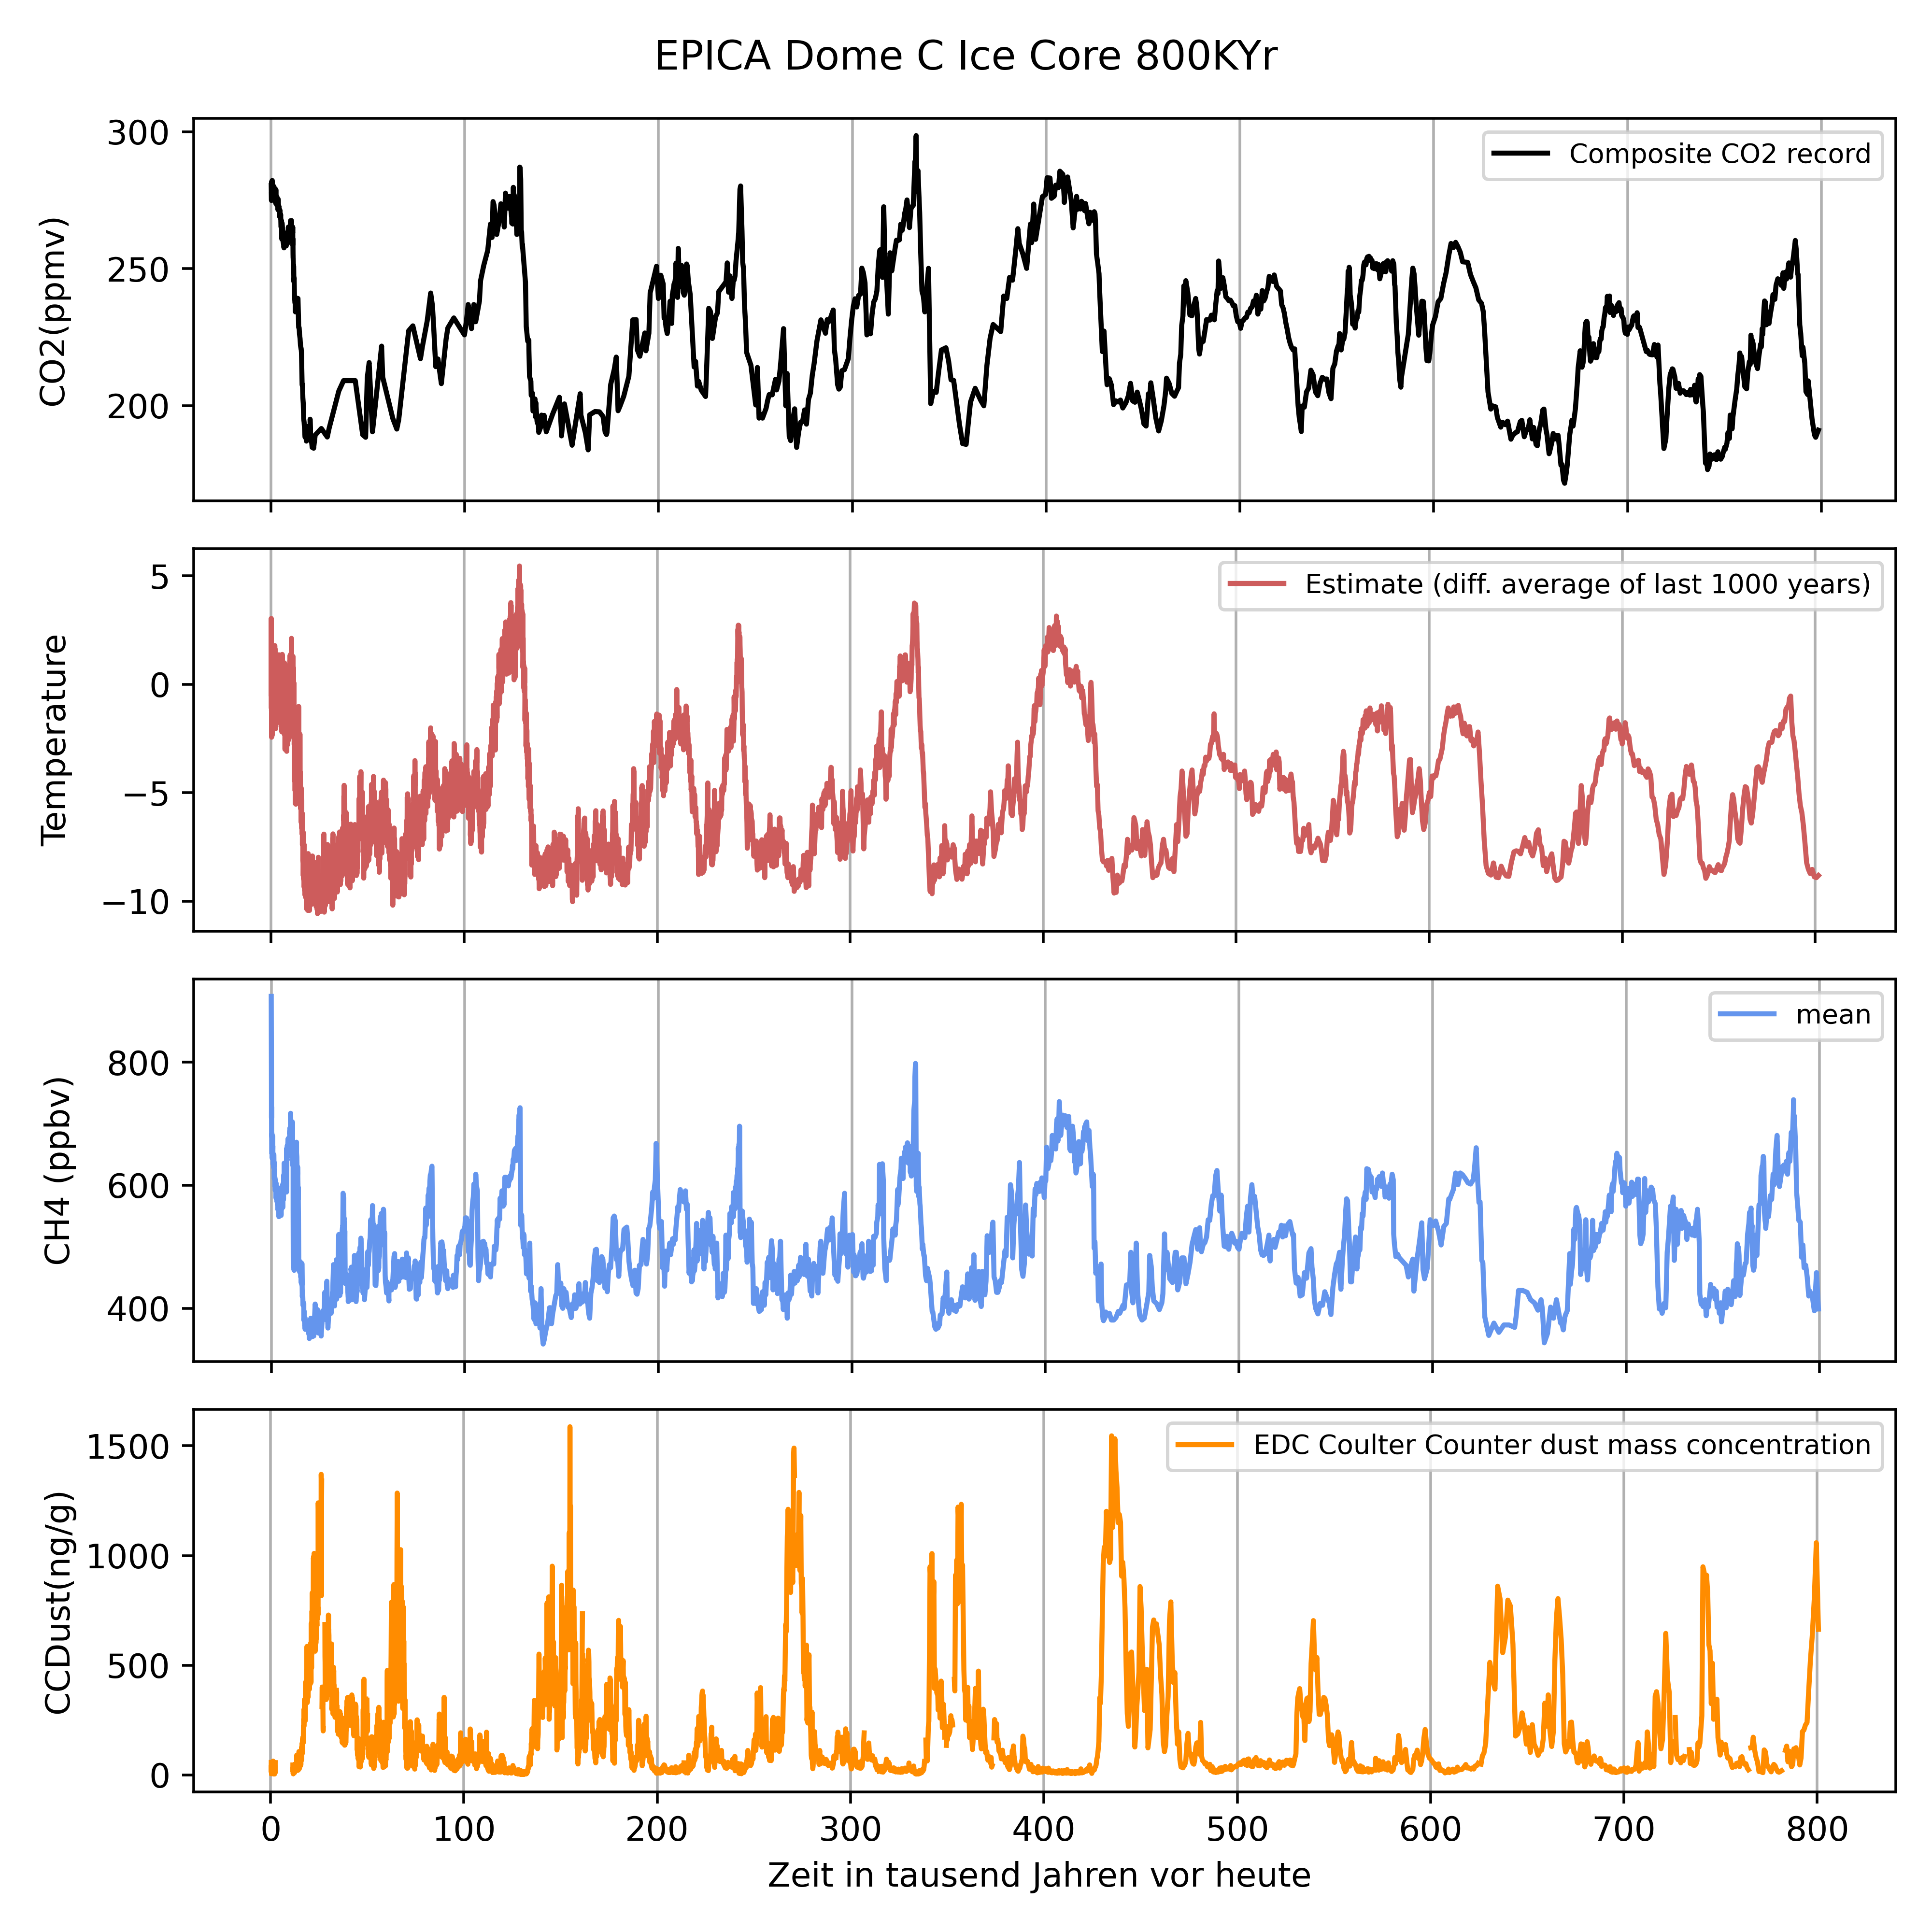
\includegraphics[width=\textwidth]{bilder/epica_icecore.png}
\caption{ Zeitreihe der letzten 800.000 Jahre für die abgeleiteten Größen \cotwo, Temperatur, Methan (CH$_4$) und Staubkonzentrationen. Erstellt aus den Datensätzen von \cite{Jouzel.2007}, \cite{Lambert.2012},\cite{Loulergue.2008},\cite{Bereiter.2015}, zur Verfügung gestellt über das \textit{National Climatic Data Center (NCDC) }  }   \label{fig:icecore}
\end{figure}

\subsection{Der südliche Ozean und die Eisenhypothese} \label{sec:Eisenhypothese}
Der Austausch von Staub und \cotwo \ hat rund um die Antarktis eine besondere Bedeutung. Einige Modelle können die regelmäßigen und \textit{globalen} Klimaveränderungen im derzeitigen Eiszeitalter  ausschließlich mit Prozessen des südlichen Ozeans erklären \citep{Fischer.2010}. Klima und Wetter nördlich des antarktischen Kontinents werden stark durch den  Zirkumpolarstrom \textit{(ACC, Antarctic Circumpolar Current)} beeinflusst. Der ACC umströmt die Landmasse zyklonal und ist gemessen an den Wassermassen die größte und für die globale Klimadynamik vermutlich wichtigste Meeresströmung überhaupt. Es wird davon ausgegangen, dass in dieser Region ein großer Teil der globalen Erwärmung umgesetzt wird. Darüber hinaus sind die Ozeane verglichen mit der Atmosphäre wahre \cotwo \ Speicher und nehmen einen Großteil (ca. 20-30 \%, vgl. \citep{IPCCpol.2019}) der anthropogenen \cotwo \ Emissionen auf, wovon schätzungsweise etwa 40 \% auf diese Region entfallen \citep{Boning.2008}. Dies führt zu einer zunehmenden \textit{Versauerung} der Ozeane sodass der pH-Wert durch diese Entwicklung in diesem Jahrhundert weiter signifikant sinken wird \citep{IPCCpol.2019}. Der ACC verbindet Atlantik, Pazifik und den indischen Ozean miteinander, was den Austausch von Wassermassen (und die globale thermohaline Zirkulation) überhaupt erst ermöglicht. Angesichts der enormen Relevanz dieser Region ist es wahrscheinlich, dass sämtliche Prozesse, die Einfluss auf ebendiese nehmen, auch weitreichende Folgen für das globale Klima haben können. \\

Grundsätzlich ist der südliche Ozean ein nährstoffreiches Gebiet. Der durch den zyklonalen ACC angetriebene \textit{Ekman-Transport} befördert das durch die \textit{Westerlies} initial angetriebene Oberflächenwasser nordwärts. Dieser Export wird südlich ausgeglichen, indem Wasser aus größeren Tiefen aufsteigt. Dieses an die Oberfläche beförderte Tiefenwasser ist i.d.R. nährstoffreicher als das Oberflächenwasser, da dessen Nährstoffe nicht permanent von der in der euphotischen Zone üppigeren Fauna konsumiert werden. Trotz dieses Nährstofftransports sind die dortigen Konzentrationen des Phytoplanktons im Mittel geringer, als man ursprünglich erwartet hatte. Derartige Zonen mit hohem Nährstoffgehalt aber geringem Aufkommen von chlorophyllhaltigem Phytoplankton werden allgemein als HNLC (high nutrient low chlorophyll) Regionen bezeichnet. Es wurde bereits früh vermutet, dass unterschiedlicher Bedarf und Verfügbarkeit an Nährstoffen die Ursache für das gehemmte Wachstum ist. Der Nährstoffbedarf der Organismen ist sehr komplex und selbst heute sind noch nicht alle Zusammenhänge vollständig verstanden (sh. Kapitel \ref{sec:Phytoplankton}). Ein Nährstoffe mit zahlreichen Abhängigkeiten ist Eisen. Spätestens nachdem Ende der 1980'er im Nordosten des subarktischen Pazifiks gezeigt werden konnte, dass die künstliche \textit{Düngung} von Wasserproben mit Eisen zu einem deutlichen Anstieg der Phytoplanktonproduktion führen kann, war evident, dass Eisen ein wichtiger Nährstoff für Phytoplankton ist und dessen Wachstum limitieren kann \citep{Martin.1988}. Dieser Tatbestand war nicht überraschend, da der Eisenbedarf (als Nährstoff) für beliebige lebende Organismen bereits hinreichend bekannt war. Bis dato war der Nachweis für Phytoplankton allerdings methodisch schwierig \citep{Martin.1988}. Insbesondere auf Basis dieses damals neuen Nachweises wird schließlich die Eisenhypothese formuliert. \\

Wie weiter oben beschrieben, übernimmt der südliche Ozean in der globalen Klimadynamik eine wichtige Rolle. Klimatische Änderungen in dieser Region korrelieren stark mit den natürlichen \cotwo -Konzentrationen der letzten 800.000 Jahre \citep{Fischer.2010}. In diesem Rahmen übt Phytoplankton direkt Einfluss aus, da im Rahmen der Fotosynthese \cotwo \ konsumiert, also der Atmosphäre / dem Ozean entzogen, und dabei in organische Kohlenstoffverbindungen (Glukose) und Sauerstoff umgesetzt wird. Während dieser \textit{Wachstumsphase} werden die umgebenden \cotwo \ Konzentrationen demnach reduziert. Sorgen nun weitere Prozesse wie die \textit{Biologische Pumpe} (sh. Kapitel \ref{sec:biopump}) dafür, dass der organisch gebundene Kohlenstoff dauerhaft von der Atmosphäre separiert wird, können die \cotwo \ Konzentrationen durch erhöhte Produktion von Phytoplankton langfristig reduziert werden. Potential für steigende Produktionsraten hat speziell der südliche Ozean als größte HNLC-Region. Könnten die überschüssigen Nährstoffe in großen Teilen dieser Region komplett durch Phytoplankton konsumiert werden, würde dies die globalen atmosphärischen \cotwo \ Konzentrationen erheblich reduzieren \citep{Martin.1990}. \citet{Martin.1990} argumentiert, dass das Wachstum von Phytoplankton im heutigen südlichen Ozean mangels biologisch verfügbarem Eisen limitiert ist. Ferner wird postuliert, dass ein nennenswerter Anteil der in Abb. \ref{fig:icecore} beschriebenen Variationen der \cotwo \ Konzentrationen zwischen Glazialen und Interglazialen aus der jeweilig unterschiedlichen Verfügbarkeit von Eisen resultiert. Der während der Glaziale höhere Staub- bzw. Eiseneintrag (sh. Abb. \ref{fig:co2iron}) soll entsprechend höhere Menge an Eisen in den Ozean eingebracht und so die Produktion von Phytoplankton verstärkt haben. Die dadurch wiederum erhöhten \textit{Archivierungsraten} von organischem Kohlenstoff hätten schließlich zu reduzierten \cotwo-Konzentrationen geführt. Entscheidend für diese Hypothese ist, dass im Gegensatz zu den meisten anderen Nährstoffen, äolischer Staub für küstenferne Gebiete als die dominante Hauptquelle von Eisen angenommen wird. Ebendiese Quellen sind in der südlichen Hemisphäre deutlich schwächer als auf der Nordhalbkugel \citep{Shao.2011}. Der Großteil der Hauptnährstoffe wird durch Flüsse in den Ozean eingetragen, welche die Produkte der Verwitterungsprozesse von den Landmassen abtransportieren \citep{Emerson.2009}. \citet{Tagliabue.2017} fassen zusammen, dass neben dem Eintrag von eisenhaltigen Staub inzwischen weitere Prozesse für die Verteilung des biolgisch verfügbaren Eisens (sh. Kapitel \ref{sec:Phytoplankton}) im Ozean anerkannt sind und insbesondere in höheren Breiten gegenüber dem Staubeintrag dominieren können. Neben diesem indirekten \textit{düngenden} Effekt kann Staub potentiell auch direkten Einfluss auf den Kohlenstofffluss in Richtung Tiefsee nehmen, indem Staubpartikel mit organischem Material im Oberflächenwasser aggregieren und die Sinkgeschwindigkeit damit  erhöhen \citep{vanderJagt.2018} . \\

Die Eisenhypothese wurde inzwischen in mehreren Experimenten getestet. Es konnte tatsächlich gezeigt werden, dass die Zufuhr von Eisen die Produktion in entsprechenden Regionen mit geringen Chlorophyll-Konzentrationen steigern kann \citep{Boyd.2007}. Im SOIREE (Southern Ocean Iron Release Experiment) wurden Reaktionen auf die Eisendüngung nach etwa 5 Tagen beobachtet. Hauptsächlich wurde das Wachstum größerer Kieselalgen gefördert \citep{Trull.2001}. Es konnte allerdings nicht gezeigt werden, dass ebenfalls der Export durch die \textit{Biologische Pumpe} erhöht wurde. In vielen Regionen scheint dieser zusätzlich durch die Verfügbarkeit von Silizium limitiert. Die sogenannte \textit{Silizium-Pumpe} (beschleunigtes Absinken des Phytoplanktons durch erhöhte Dichte aufgrund der Siliziumdioxid-Frusteln, vgl. Abschnitt \ref{sec:biopump}) arbeitet bereits am Limit. Obwohl geschätzt wird, dass bei etwa 40 \% des ozeanischen Oberflächenwassers Eisen ein limitierender Faktor für die Produktion von Phytoplankton sein kann \citep{Emerson.2009}, wird der Beitrag des durch äolischen Eisens (durch Staub) inzwischen geringer eingeschätzt \citep{Tagliabue.2017}. \citet{Vallelonga.2013} schätzen diesen Beitrag zur Variabilität nach dem letzten glazialen Maximum (LGM) auf maximal 20 ppmv \cotwo . Lässt sich (wie im Rahmen dieser Arbeit untersucht) zeigen, dass die vergleichsweise (ggü. nördl. Hemisphäre) seltenen Staubereignisse einen entsprechenden Einfluss nehmen, wäre dies in diesem Zusammenhang ein wichtiger Mechanismus und Indiz für eine höhere Relevanz des äolischen Staubs.

\begin{figure}
\centering
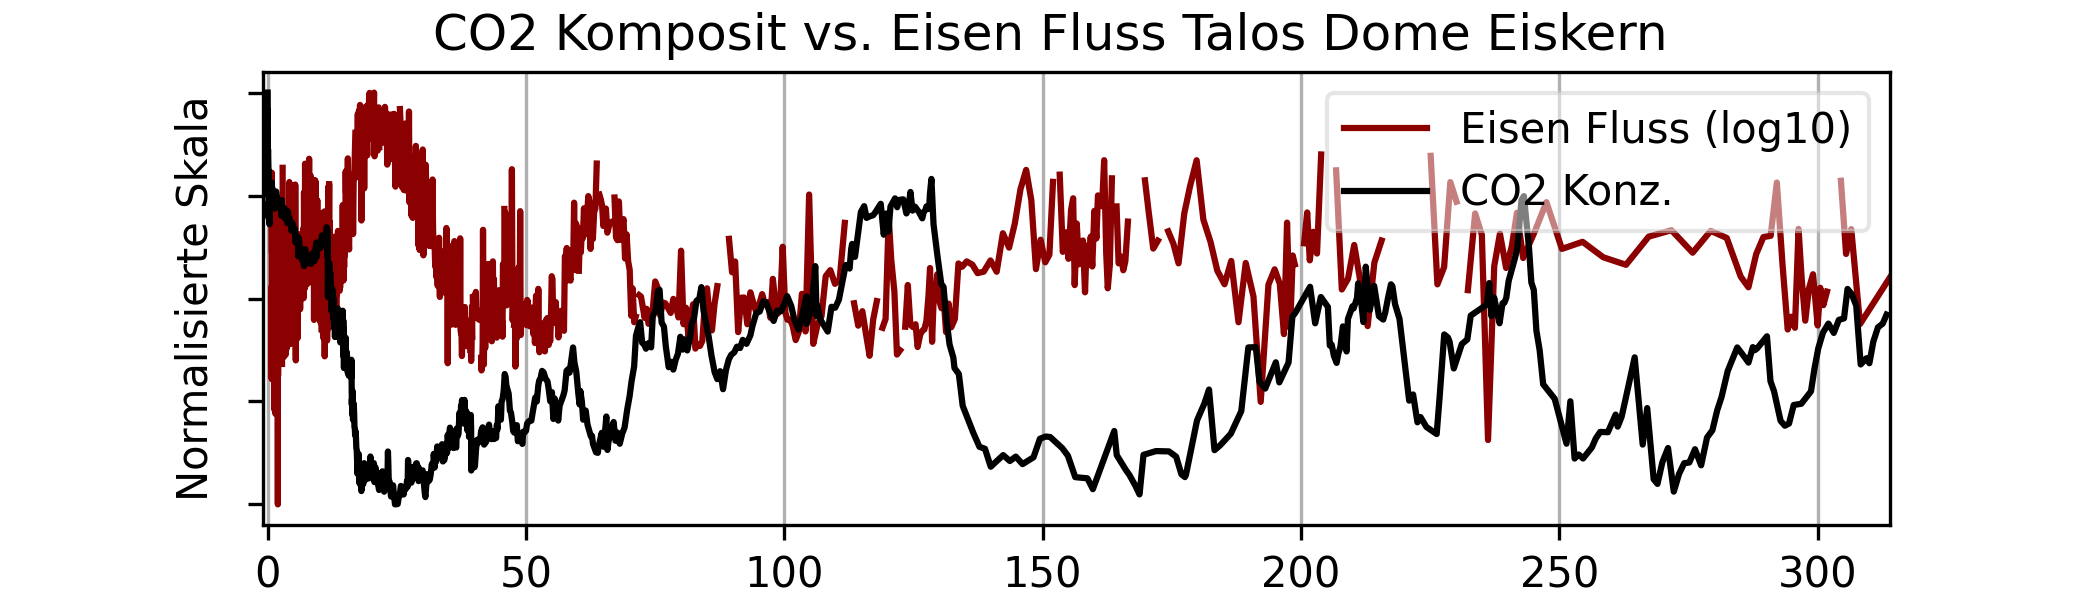
\includegraphics[width=\textwidth]{bilder/co2_iron.png}
\caption{ Zeitreihe der letzten 314.000 Jahre für die abgeleiteten Größen \cotwo (dunkelrot) und den Eisenfluss, die zur Eisenhypothese inspirierte. Die Größen weisen insbesondere während der kälteren Glaziale eine starke Antikorrelation auf. Abnehmende \cotwo -Konzentrationen gehen mit erhöhtem Eisenfluss einher. Erstellt aus den Datensätzen von \cite{Bereiter.2015} und \cite{Vallelonga.2013}, zur Verfügung gestellt über das \textit{National Climatic Data Center (NCDC) }  }   \label{fig:co2iron}
\end{figure}

\subsection{Eigenschaften und Abhängigkeiten von Phytoplankton} \label{sec:Phytoplankton}
Bis hierhin wurde Phytoplankton bereits häufig erwähnt und diskutiert, tatsächlich aber noch nicht angemessen vorgestellt. Aufgrund der enormen Bedeutung sollen in diesem Abschnitt die grundsätzlichen Eigenschaften und einige der besonderen komplexen Zusammenhänge separat aufgezeigt werden. Eine seriöse Analyse der Entwicklung der Phytoplankton Konzentrationen ist ohne diese entsprechende Berücksichtigung kaum möglich. 
\subsubsection{Allgemeines zu Phytoplankton} \label{sec:Phytobasics}
Durchschnittlich ungefähr 10 µg pro Liter bzw. $10^{-6}$ Prozent des Oberflächenwassers bestehen aus lebenden Organismen \citep{Emerson.2009}. Obwohl diese Konzentration weitaus geringer als an Land ist, nehmen Kleinstorganismen wie Phytoplankton einen erheblichen Einfluss auf ihre Umwelt. Neben dem enormen Einfluss auf die Atmosphäre (sh. Kapitel \ref{sec:Eisenhypothese}) bilden diese einzelligen und autotrophen (sich nur vom Sonnenlicht \textit{ernährenden}) Lebewesen die ultimative Basis der Nahrungskette. Die Lebenserwartung von Phytoplankton beträgt gerade einmal Stunden bis hin zu Tagen. Dieses Mikroleben entspricht aufgrund der sehr kurzen Zeitspanne in der Zusammensetzung praktisch ausschließlich dem Zustand des lokalen Ozeanwassers und kann besser durch die hinterlassenen chemischen Spuren beobachtet werden als durch direkte Untersuchung. Neben der Verfügbarkeit von Nährstoffen wird der Bestand durch das in der Nahrungskette nächsthöhere Zooplankton reguliert, welches sich von Phytoplankton ernährt. \citet{Boyce.2010} folgern, dass der Reichtum an Phytoplankton insgesamt seit Beginn der Messungen (1899) aufgrund der Erwärmung der Ozeane abgenommen hat. Es wird geschätzt, dass das globale Median jährlich um etwa 1\% abnimmt. Da die Klimamodelle steigende (Meeres-)Temperaturen prognostizieren ist es wahrscheinlich und problematisch, dass die Menge an Phytoplankton, der Basis aller Nahrungsketten im Ozean, zukünftig noch weiter abnimmt \citep{Siegel.2010}. Klimaänderungen werden direkt (andere Ozeanchemie) und indirekt (Änderungen in der Ozeanzirkulation) die Verteilung des Phytoplanktons verändern \citep{Falkowski.1998}.  

Je nach Region und Jahreszeit wird das Ozeanwasser durch verschiedene Unterarten des Phytoplankton repräsentiert. Die das Picophytoplankton ($<2\mu$m) in vielen Teilen des Ozeans dominierenden Cyanobakterien \textit{Synechococcus} und \textit{Prochlorococcus} enthalten vermutlich am meisten der grünen, Licht absorbierenden Pigmente (Chlorophyll) \citep{Emerson.2009}. \textit{Kieselalgen} dominieren in Regionen, in denen aufsteigendes Wasser nennenswerten Einfluss nimmt, wie bspw. im südlichen Ozean. Dort besteht das Sediment größtenteils aus den \textit{Frusteln} (Schalen, bestehen überwiegend aus Siliziumdioxid SiO$_2$) der Kieselalgen. Für Kieselalgen ist die Zufuhr von Kieselsäure daher essenziell; diese tritt fast ausschließlich südlich der Südpolarfront auf \citep{Falkowski.1998}.

\subsubsection{Nährstoffe} \label{sec:nährstoffe}
Auch autotrophe Organismen benötigen neben dem einfallenden Sonnenlicht weitere Nährstoffe um zu wachsen. Diese werden in Makro- und Mikronährstoffe unterteilt. Die Makronährstoffe Kohlenstoff (C), Stickstoff (N) und Phosphor (P) sind Arten-übergreifend die Hauptbestandteile des Phytoplanktons. Diese werden ungefähr im Verhältnis (106C/16N/1P) konsumiert \citep{Falkowski.1998}. Eine abgeleitete näherungsweise, nicht allgemeingültige Formel für die Fotosynthese  \citep{Emerson.2009} veranschaulicht die chemische Zusammensetzung und den Nährstoffbedarf:
\begin{equation}
\text{106\cotwo} + \text{16HNO}_3 + \text{H}_3\text{PO}_4 + \text{122H}_2\text{O} \rightarrow \text{(CH}_2\text{O)}_{106}\text{(NH}_3\text{)}_{16}\text{H}_3\text{PO}_4 + \text{138O}_2
\end{equation}
Neben diesen relativ gut bekannten Abhängigkeiten von den Makronährstoffen sind die in viel geringerer Menge notwendigen (und verfügbaren) Mikronährstoffe aber genauso wichtig und können das Wachstum limitieren. Hierzu gehören beispielsweise Spurenelemente wie Mangan, Eisen, Kobalt, Nickel, Kupfer und Zink. Ein Teil dieser Metalle wird durch (mutmaßlich aus biologischen Prozessen entstandenen) Liganden komplexifiziert bzw. besetzt und können die biologische Verfügbarkeit für das Phytoplankton einschränken. Die Natur dieser Liganden ist noch nicht vollumfänglich verstanden, allerdings wird davon ausgegangen, dass ausschließlich die weiterhin \textit{freien} Metalle biologisch verfügbar sind \citep{Emerson.2009}. Darüber hinaus können diese aber auch dazu führen dass bspw. Eisen in gelöster Form verbleibt, also nicht absinkt/aggregiert, und über größere Strecken transportiert werden kann \citep{Tagliabue.2017}. Berücksichtigt man diese weiteren Mikronährstoffe, lässt sich wieder ein stöchiometrisches Verhältnis ableiten, dass an dieser Stelle wieder nicht exakt oder allgemein gilt, sondern nur die Größenordnungen der Beiträge exemplarisch aufzeigen soll \citep{Emerson.2009}:
\begin{equation}
\text{(C}_{106} \text{N}_{16} \text{P)}_{1000} \text{Fe}_8\text{Mn}_4\text{Zn}_{0.8}\text{Cu}_{0.4}\text{Co}_{0.2} \text{Cd}_{0.2}
\end{equation}
Insbesondere der Bedarf an Eisen kann je nach Umgebung höchst unterschiedlich sein. Es wurde beobachtet, dass die Entwicklung des Phytoplanktons von allen Nährstoffen entsprechend dem Minimum-Gesetz (\textit{Liebig's Law}) abhängt. Demnach ist das Wachstum durch den Nährstoff beschränkt, der im entsprechenden Verhältnis am wenigsten verfügbar ist. Dadurch bilden sich die bereits in Kapitel \ref{sec:Eisenhypothese} HNLC-Regionen, in denen zwar viele Nährstoffe im Überfluss vorhanden sind, jedoch nicht konsumiert werden können, weil ein Baustein fehlt. Diese Beobachtung ist für die Eisenhypothese wesentlich, wonach der Nährstoff Eisen für den Großteil dieser ungenutzten Potentiale verantwortlich sein soll. \citet{Martin.1988} zeigten zunächst exemplarisch für eine Region in isolierten Behältern, dass die übrigen Nährstoffe nach Zugabe von Eisen etwa 4 Tage später tatsächlich konsumiert wurden. Es wird geschätzt, dass bei etwa 40 \% des ozeanischen Oberflächenwassers Eisen ein limitierender Faktor für die Produktion von Phytoplankton sein kann \citep{Emerson.2009}. Aufgrund des Konsums durch Phytoplankton sind Eisen und andere Nährstoffe  an der Ozeanoberfläche häufig im Vergleich zu tieferen Schichten (in welchen das Licht-abhängige Phytoplankton nicht überlebt) reduziert \citep{Martin.1990}. Andere Nährstoffe  können durch aufsteigendes Tiefenwasser bereitgestellt werden. Eisen und Mangan werden hingegen zu nennenswerten Teilen durch äolischen Staub eingebracht. Ansonsten sind grundsätzlich Flüsse die Hauptquelle für gelösten Eintrag von Elementen \citep{Emerson.2009} Die Konzentrationen des Elements Eisen im Meerwasser sind verglichen mit den häufigsten Stoffen wie Natrium, Chlorid, Sulfat und Magnesium sehr gering. Dennoch ist es das dritthäufigste Element in marinen Sedimenten. \citep{Emerson.2009}. Wie lange Eisen in den oberen Schichten verbleibt, hängt vordergründig von dessen Zustand ab. In gelöster Form sinkt es kaum und kann etwa 6 Monate in Tiefen bis max. 150m residieren \citep{Hayes.2015}. In Form von Aggregaten und größeren Partikeln ist die Sinkgeschwindigkeit jedoch deutlich höher. In einer Fallstudie für einen vorangegangenen Staubsturm gehen \citet{Boyd.2010} von einer Verweilzeit in oberflächennahen Schichten von 30 Tagen für äolisch eingebrachtes Eisen aus. Darüber hinaus ist Eisen nicht in jeder Form biologisch verfügbar. Insbesondere innerhalb von Staub kommt Eisen in der kaum löslichen Form Fe$^\text{3+}$ vor anstatt des gut löslichen Fe$^\text{2+}$ \citep{Reynolds.2014}. \\

Neben dem Einfluss als direkter Nährstoff kann Eisen das Wachstum von Phytoplankton noch in Form von Enzymkomplexen fördern. Nitrogenase kann N$_2$ reduzieren und Stickstoff biologisch verfügbar machen. Der Einfluss ist also nicht auf die sogenannten HNLC-Regionen beschränkt und kann auch in solchen mit wenig verfügbarem Stickstoff (LNLC) wirken. Die Zugabe von Eisen fördert, dass Nitrate (NO$_3^-$) zu Ammonium-Ionen (NH$_4^+$) reduziert werden, welche bei der Fotosynthese von Plankton mit hohem Bedarf an Nitraten besonders schnell verwendet werden können.  \citep{Emerson.2009}. Laut \citet{Emerson.2009} ist dies das extremste Beispiel, für die Limitierung durch Eisen, da diese Enzyme zu einem großen Teil aus Eisen bestehen. Nitrogenase selbst benötigt (bzw. besteht aus) Eisen. Diese Funktion wurde insbesondere bei der diazotrophen Phytoplankton-Art \textit{Trichodesmium} beobachtet. \citep{Falkowski.1998}.  In nährstoffarmen Gewässern haben derartige extrem kleine Phytoplankton-Organismen bei der Verarbeitung von Nährstoffen (Exkrementen der Verbraucher)  aufgrund des größeren Oberflächen zu Volumen- Verhältnisse einen Wettbewerbsvorteil \citep{Falkowski.1998}. Wenn hingegen \textit{neue} Nährstoffe bspw. durch Aufströmen in das lichtdurchflutete Oberflächenwasser gelangen, hat größeres Phytoplankton, insbesondere Kieselalgen einen Wettbewerbsvorteil (aufgrund Vakuole, schnellere Aufnahme). Entsprechende \textit{Blooms} (wie bei Eisendüngung) bestehen dadurch häufig aus Kieselalgen \citep{Boyd.2007}. Das Plankton, das sich wiederum von diesen ernährt, ist typischerweise größer, benötigt für Entwicklung (Larvenstadium) mehr Zeit wodurch Blooms möglich sind. Die Biologische Pumpe (Kapitel \ref{sec:biopump}) wird entsprechend intensiviert. \\

Im südlichen Ozean kann auch Mangan ein limitierender Nährstoff sein \citep{Browning.2021}. Bisher wurde Mangan diesbezüglich nicht verdächtigt. Die Besonderheit bei Mangan ist, dass dieses Spurenmetall im Gegensatz zu Eisen kaum durch Liganden besetzt wird und damit wesentlich mehr biologisch verfügbar ist \citep{Emerson.2009}. 
\subsubsection{Biologische Pumpe} \label{sec:biopump}
Das Ökosystem innerhalb der euphotischen Zone ist höchst effizient. Die im Phytoplankton enthaltenen Nährstoffe werden nach dem Absterben oder \textit{Abgrasen} durch Zooplankton sehr schnell wieder remineralisiert und für die nächste Generation in der Nahrungskette verwendet. Entsprechend wenig Material entkommt den oberflächennahen Schichten. Durch temporär erhöhte Phytoplankton-Konzentrationen alleine erfolgt daher noch keine dauerhafte Archivierung des Kohlenstoffs, obwohl dieses zunächst bei der Photosynthese in organischem Material gebunden wurde. Nur wenn dieses bis auf den Meeresgrund sinkt ist es dem Kreislauf der Wiederfreisetzung für bis zu mehrere tausend Jahre entzogen. Dieser Prozess, bei dem organischer Kohlenstoff absinkt, wird \textit{Biologische Pumpe} genannt. Der Export von organischer Materie aus der euphotischen Zone ist für den Hauptteil der chemischen Prozesse in der Tiefsee verantwortlich \citep{Emerson.2009}. Ein niedriger Sauerstoffgehalt in der Tiefsee weist auf starke biologische Pumpe hin. Der so beförderte organische Kohlenstoff wird zersetzt, wodurch \cotwo \ freigesetzt und Sauerstoff konsumiert wird (umgekehrte Fotosynthese, \cite{Honjo.2008}). Im aktuellen Ozean beträgt der durchschnittliche (Sink)Fluss zwischen dem Meso- und Bathypelagial in etwa 2 km Tiefe ca. 0.84 Pg Kohlenstoff (organisch+anorganisch) pro Jahr \citep{Honjo.2008}. Aufgrund der höheren Dichte von Mineralen (vereinfachend angenommen ca. $2.5$ g/cm$^{-3}$) im Gegensatz zu organischer Materie (ca. $1.1$ g/cm$^{-3}$) und Meerwasser (ca. $1$ g cm$^{-3}$) kann abgeschätzt werden, dass anorganische Partikel etwa 15 mal schneller sinken als rein organische. Entsprechend kann abgeleitet werden, dass Organismen ohne zusätzlichen mineralischen Ballast aufgrund der geringen Sinkgeschwindigkeit die euphotische Zone praktisch kaum verlassen können. Zusätzlich bietet eine mineralische Hülle entsprechenden Schutz vor Oxidation der organischen Materie, die ansonsten bereits innerhalb der ersten 2000m während des Sinkens einsetzen würde\citep{Emerson.2009}. Demzufolge können Blooms derjenigen Unterarten des Phytoplankton wie Kieselalgen und Coccolithoporida, die sogenannte Frusteln aus Siliziumdioxid respektive Kalziumkarbonat bilden die biologische Pumpe temporär beschleunigen. Es wird angenommen , dass die Leistung der biologischen Pumpe (d.h. der Sinkfluss) aufgrund der Klimaveränderungen insgesamt global abnehmen wird. Auch der wichtige Nährstoff Eisen wird im Rahmen der biologischen Pumpe recycelt und teilweise in die Tiefsee befördert. Da die Remineralisierung (das \textit{verfügbar machen}) länger dauern kann als bei anderen Elementen, wird Eisen diesem Kreislauf tendenziell schneller wieder entzogen. Darüber hinaus führt hoher Sauerstoffgehalt zu einer schnellen Oxidation des Eisens, welches dadurch kaum noch löslich ist und sinkt \citep{Falkowski.1998}. Diese  Effekte tragen zur Eisenarmut des Oberflächenwassers vieler Regionen bei.
\subsubsection{Meeresströmungen und Mixed Layer}
Wie in den vorangegangenen Kapiteln beschrieben, hängt die Entwicklung des Phytoplanktons neben der zur Fotosynthese unerlässlichen Sonneneinstrahlung von der Verfügbarkeit der Nährstoffe ab. Diese Verfügbarkeit wird wiederum durch Meeresströmungen gesteuert. Die Mischschicht des Oberflächenwassers (englisch \textit{Mixed Layer}) bezeichnet die Zone des Oberflächenwassers, in welcher die Bestandteile (auch das Phytoplankton) des Meerwassers größtenteils homogen durchmischt werden. Die Veränderung der Tiefe dieser Mischschicht (MLD, \textit{Mixed Layer Depth} kann sowohl positive als auch negative Auswirkungen auf die Entwicklung des Phytoplanktons haben: Durch eine Vertiefung werden weitere Meeresschichten, deren Nährstoffe bisher weniger konsumiert wurden einbezogen, sodass sich der durchschnittliche Nährstoffgehalt erhöhen kann. Gleichzeitig erreicht den tieferen Teil der Mischschicht weniger Sonnenlicht, sodass dies ein limitierender Faktor für die Entwicklung des Phytoplanktons sein kann. Ein Abflachen der MLD geht häufig mit erhöhter Sonneneinstrahlung einher, welche das Oberflächenwasser thermodynamisch stabilisiert und stratifiziert. Dann steht zwar mehr Sonnenlicht zur Verfügung, die Nährstoffe werden aber (bis zur Limitierung durch den am wenigsten verfügbaren Nährstoff) schneller aufgebraucht. Aufgrund der jahreszeitlich variierenden Sonneneinstrahlung folgt die MLD vielerorts einem jahreszeitlichen Gang, welcher in Abbildung \ref{fig:mld_currents} beispielhaft für den südlichen Ozean dargestellt ist. Die zunehmende Sonneneinstrahlung mit einsetzen des Frühlings im September führt zu einer deutlich reduzierten MLD. Im tasmanischen Meer fördert dieser Trend Phytoplanktonblüten im Frühling \citep{Tilburg.2002}. Neben der MLD können dort Wirbel (\textit{Eddies} einen erheblichen Einfluss nehmen. Aufgrund der Corioliskraft bzw. des Ekman-Transports wird das Oberflächenwasser in zyklonalen Strömungen radial nach außen abtransportiert sodass kälteres, nährstoffreicheres Wasser aus größeren Tiefen aufströmt. Während dieser Nährstofftransport die Entwicklung des Phytoplankton innerhalb zyklonaler Wirbel fördert, führt umgekehrt die erhöhte Stratifizierung durch Kumulierung der Wassermassen in der Mitte antizyklonaler, dadurch wärmerer, Wirbel zu einer Behinderung. In Regionen wie dem tasmanischen Meer, in welchem aufgrund des östlich abgelenkten Ostaustralstroms (EAC, \textit{East Australian Current} besonderes ausgeprägte Wirbel entstehen, können diese Effekte zu einem sehr heterogenen Muster der Phytoplankton-Konzentrationen führen \citep{Tilburg.2002}. Wie auf Abbildung \ref{fig:mld_currents} sichtbar, scheint der Verlauf der Strömungslinien das Muster der Chlorophyll-a Konzentrationen zu bestimmen (hierbei ist allerdings zu beachten, dass der Datensatz auf Basis des Algorithmus von \citet{Saulquin.2019} erstellt wurde, in welchem Strömungsdaten zur Interpolation der Chlorophyll-a-Konzentrationen benutzt wurden).

\begin{figure}
	\begin{minipage}[c]{0.5\textwidth}
		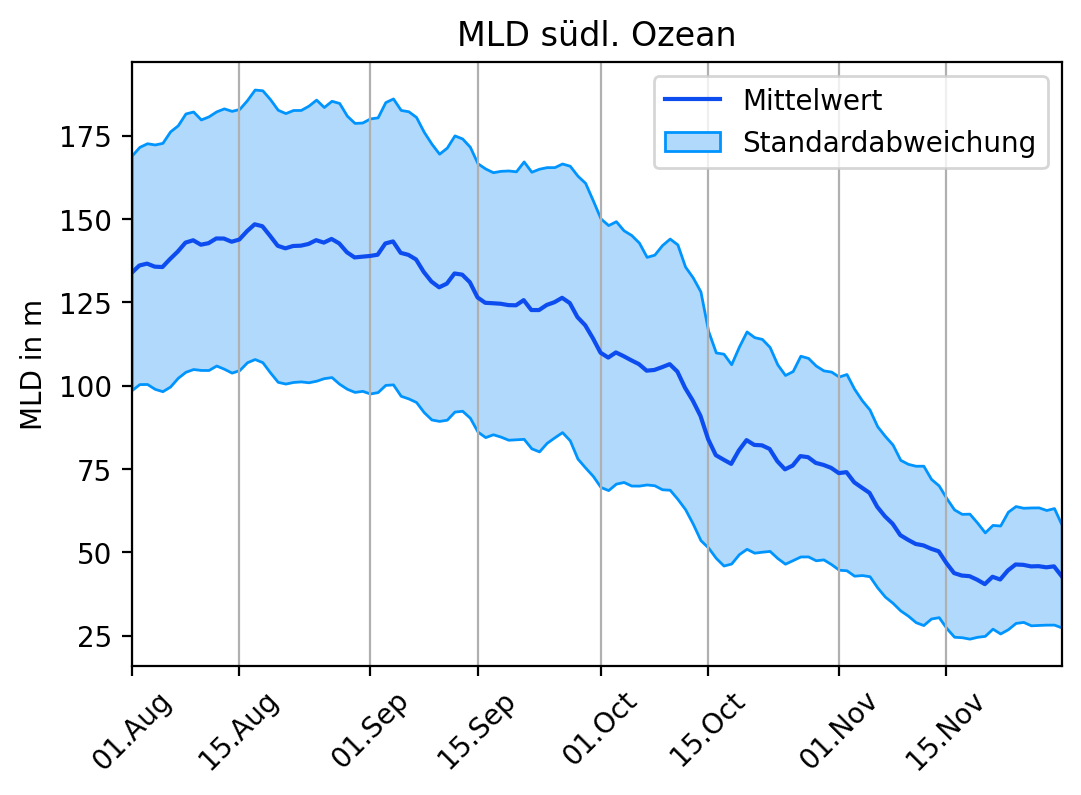
\includegraphics[width=\textwidth]{bilder/southern.png}
	\end{minipage}\hfill
	\begin{minipage}[c]{0.49\textwidth}
		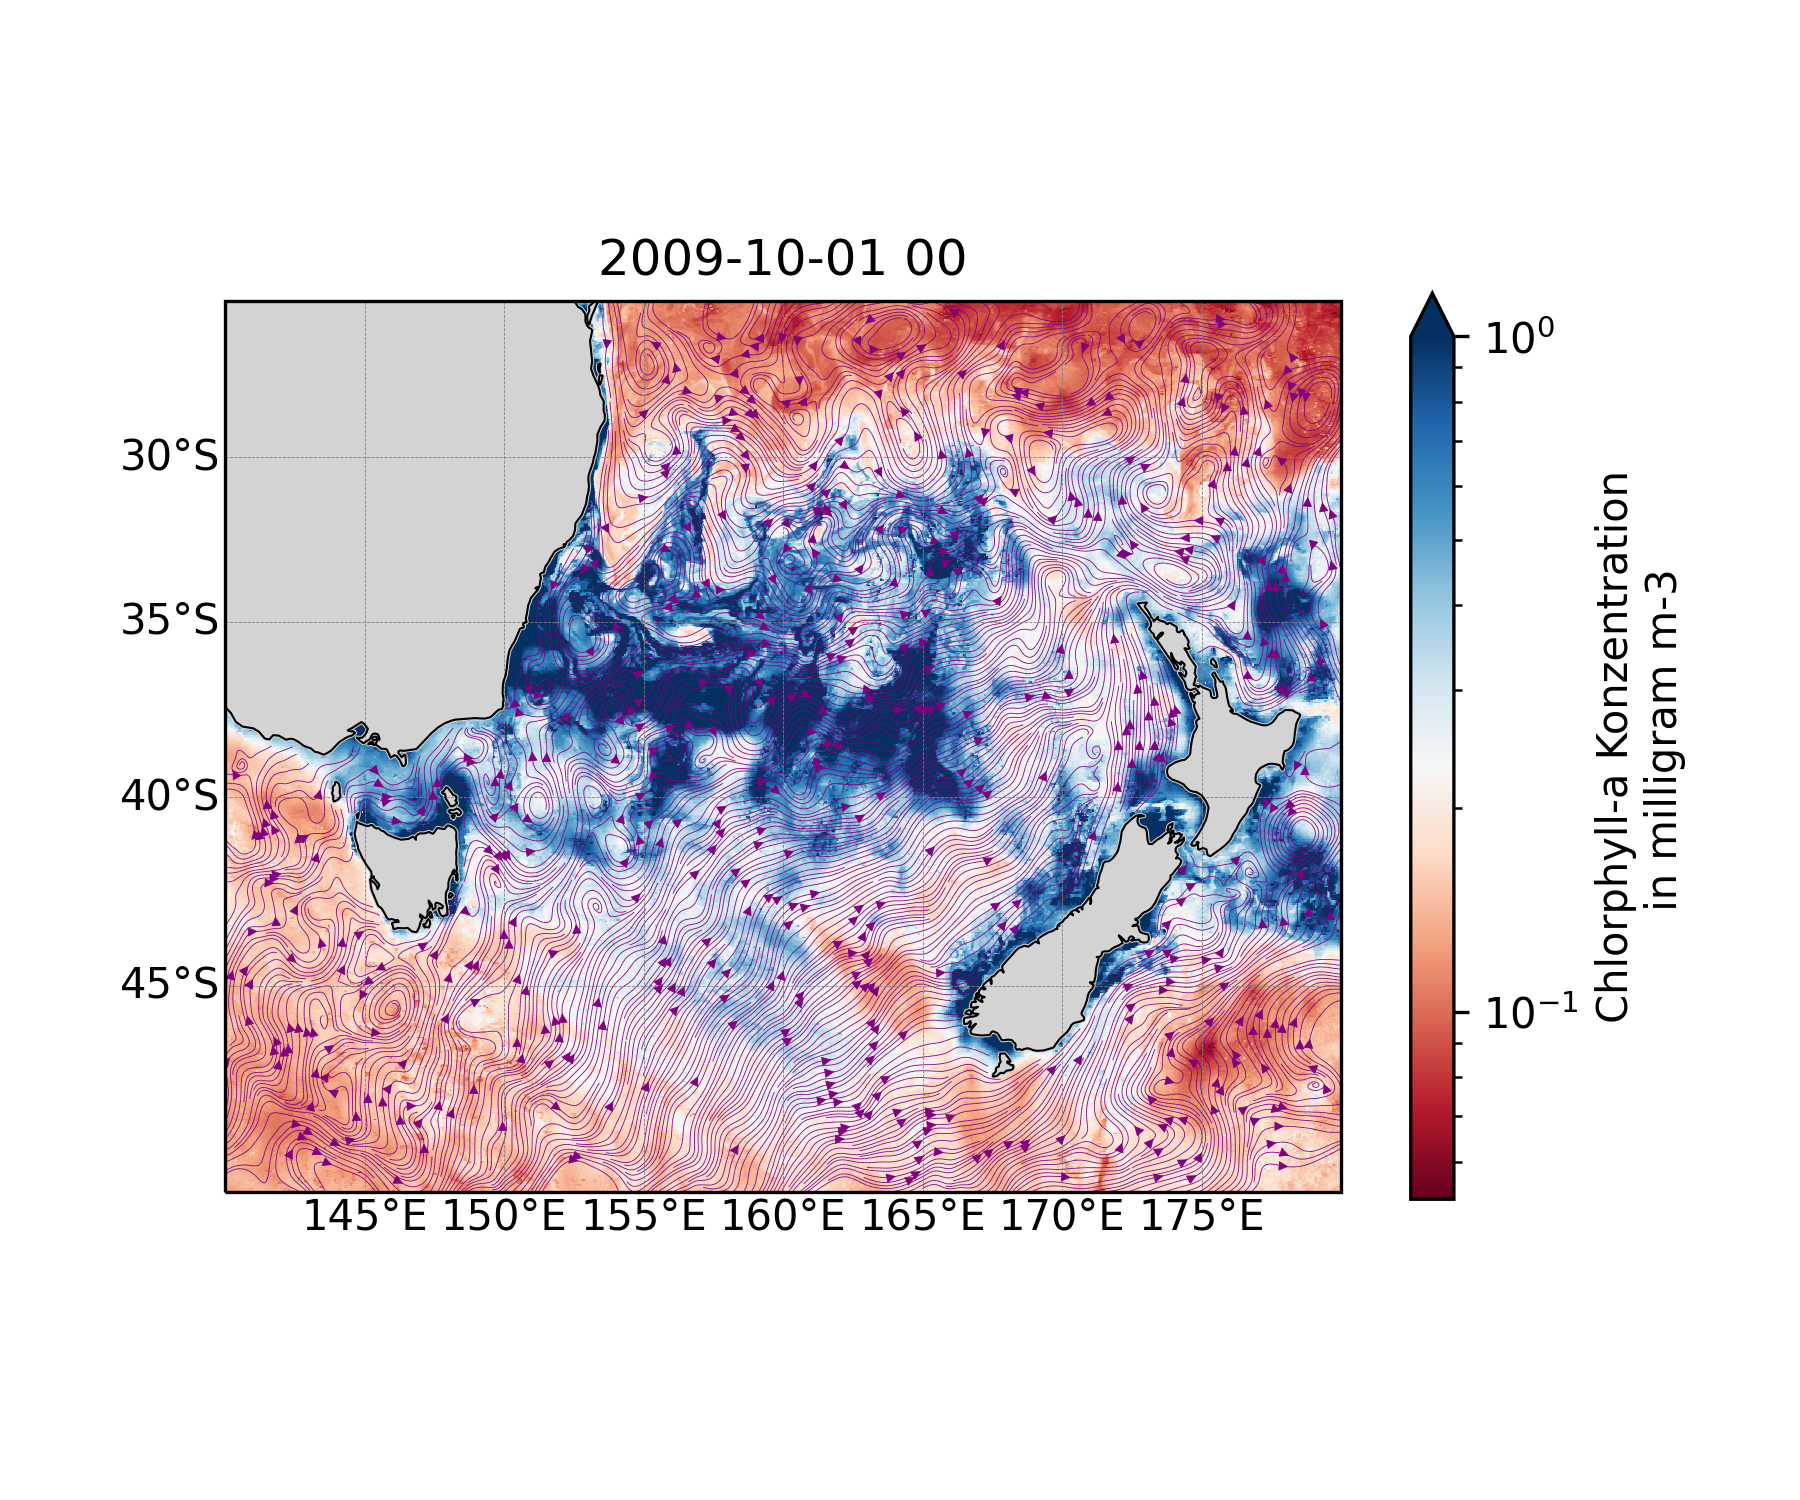
\includegraphics[width=\textwidth]{bilder/currents.png}
	\end{minipage}\hfill
	\caption{Links: mittlere MLD für einen Teil (40°E-80°W, 32°S-65°S)des südlichen Ozeans für den Zeitraum August bis Dezember. Rechts: Chlorophyll-a Konzentrationen und Strömungslinien des Oberflächenwassers für den 1. Oktober 2009. Chlorophyll-a Daten sh. Kapitel \ref{sec:chla}, Strömungs- und MLD-Daten: Copernicus Marine Service, \textit{global-reanalysis-phy-001-031-grepv2-mnstd-daily} } \label{fig:mld_currents}
\end{figure}

\subsection{Staub in Australien} \label{sec:Staub}
Die südliche Hemisphäre hat aufgrund der wenigen Landmassen auch weniger Staubquellen wodurch die Atmosphäre in Umgebung des antarktischen Zirkumpolarstroms vergleichsweise staubarm ist. Die größte Staubquelle bietet Australien \citep{Shao.2011}. In diesem Kapitel sollen die Regionen mit den höchsten Emissionspotentialen präsentiert werden (Kapitel \ref{sec:staubquellen}), um deren Einfluss bei der späteren Simulation bewerten zu können. Darüber hinaus wird in Abschnitt \ref{sec:eiseninstaub} noch einmal auf den wichtigen Nährstoff Eisen und dessen Vorkommen in Staub eingegangen. Anschließend wird das besondere Staubereignis, das sogenannte \textit{Red Dawn Event} mit den besonderen Merkmalen vorgestellt.
\subsubsection{Staubquellen in Australien} \label{sec:staubquellen}
Die Haupt- Staubquelle erstreckt sich über ein riesiges Gebiet in Zentralaustralien \citep{Shao.2011}. Das sogenannte Lake Eyre Becken liegt im Zentrum eines endorheischen Systems. Diese Eigenschaft führt dazu, dass die Bestandteile emittierten Staubs anderen Regionen entspringen können und über weite Strecken transportiert wurden. Diese Ursprünge sind i.d.R. benachbarte Regionen höherer Feuchte, in denen chemische und physikalische Verwitterung stattfindet. Während des Transports zu dem Ort, an dem der Staub später tatsächlich emittiert wird, werden die Partikel weiter zermahlen und dadurch kleiner und zusätzlich durch Winde separiert. Dementsprechend kann die Verfügbarkeit von Staub unintuitiverweise von einem ausreichend hohen (Feuchte)Fluss in die Region abhängen, anstatt von ausschließlicher anhaltender Dürre \citep{Marx.2018}.
Laut \citet{Deckker.2019} sind \textit{Kati Thanda-Lake Eyre} Region und \textit{Darling Riverine Plain} (Oberlauf des Darling River) Hauptquellen. Der Kontinent deckt insgesamt ein breites Spektrum an Oberflächengeologie ab, sehr alte Landmasse; einige Flächen sind mehr als 2.5 Milliarden Jahre alt (aus dem Archean). Durch die Besiedelung und Landnutzung durch den Menschen haben sich signifikante Änderungen ergeben, die bis 1945 mutmaßlich zu einer höheren Frequenz an Staubstürmen geführt haben. Nach verbesserter Landnutzung nahmen auch die Staubstürme wieder ab \citep{Deckker.2019}. Größte Staubereignisse vor 2009 waren in den 1940'er Jahren. Staub entstammt nicht nur ariden Wüstengebieten. Ein nennenswerter Anteil ($>$ 5\%) entsteht in kalten/glazialen Regionen hauptsächlich durch die Bewegungen von Gletschermassen und den damit verbundenen Abreibungen. Verwitterungsprozesse spielen dort im Gegensatz zu ariden Gebieten eine untergeordnete Rolle \citep{Marx.2018}.
\subsubsection{Eisen in Staub} \label{sec:eiseninstaub}
Nicht jede Form von Eisen kann als Dünger dienen. Muss entsprechend gelöstes (?) Eisen sein. Transportprozesse und Wolkenbildungen können die Transformation zu diesem tauglichen Eisen fördern \citep{Shao.2011}. Die Planktonart Trichodesmium kann die Rate des Eisenauflösens von Oxiden und Staub beschleunigen (im Gegensatz zu anderem Phytoplankton) \citep{Gabric.2016}. In Sediment enthält Staub häufig die Fe$^{3+}$ Minerale Hämatit und Goethit \citep{Reynolds.2014}. Die Ergebnisse von \citet{Reynolds.2014} legen nahe, dass der Eisengehalt (Magnetit) des Staubes beim \textit{Red-Dawn} durch die dichten urbanen Gebiete an der Küste weiter erhöht wurde.
\begin{table}[H]
\begin{tabularx}{\textwidth}{X X l}
		\toprule
			\thead{Eisenoxid(hydrate)} & \thead{Verhältnisformel} &  \thead{Vorkommen} \\
		\midrule
		Hämatit & Fe$_2$O$_3$ & Mineral, trigonales Kristallsystem \\
		Maghemit & Fe$_2$O$_3$ & Mineral, kubisches Kristallsystem \\
		Magnetit & Fe$_2$O$_4$ & Mineral, kubisches Kristallsystem \\
		Goethit & $\alpha$-Fe$^{3+}$O(OH) & Mineral, orthorhombisches Kristallsystem \\
		\bottomrule
\end{tabularx}
\caption{Beschreibung} \label{table:eisenoxid}
\end{table}

Hauptursache für die Deposition/Ablagerung von weit transportiertem Staub ist das \textit{Auswaschen} durch Regen \citep{Marx.2018}, Sekundärquelle. -
Löslichkeit \citep{Boyd.2010}. Wird Staub über mehrere tausend Kilometer transportiert, verleiben i.d.R. nur Staubpartikel mit Größen von $<$20$\mu$m \citep{Marx.2018}, Sekundärquelle.

\subsubsection{Beschreibung des Staubsturms im September 2009} \label{sec:reddawn}
Bereits nach einer schnellen Analyse im Rahmen des DustWatch Reports \citep{Leys.2009} war klar, dass es sich bei \textit{Red Dawn} um einen enormen Staubsturm mit besonderen Merkmalen handelte. Den Namen \textit{Red Dawn} erhielt dieser aufgrund der spektakulären Bilder die er am Morgen (Lokalzeit) des 23. Septembers in Sydney verursachte. Die gesamte Stadt wurde für mehrere Stunden in orange-roten Nebel gehüllt. Tatsächlich fanden im September sowohl vor als auch nach dem hier im Fokus liegenden \textit{Red Dawn} gleich mehrere Staubereignisse statt. Im ariden Inland sind Staubstürme keine Seltenheit. Dieses war allerdings vermutlich (jedenfalls in Bezug auf die Sichtweitenreduzierung) das stärkste Staubevent welches Sydney seit Beginn verlässlicher Aufzeichnungen (1940) je getroffen hat \citep{Leys.2011}. Vorangegangen sind Monate und Jahre mit im Vergleich zum Durchschnitt höheren Temperaturen und unterdurchschnittlichem Niederschlag (vgl. Abbildung \ref{fig:reddawn}), wodurch die Vegetation schwächer ausgeprägt und die Erdböden allgemein trockener waren \citep{Leys.2011}. Aufgrund der hohen Intensität wurde dieser Zeitraum \textit{Millenium Drought} getauft \citep{Deckker.2014}.
\begin{figure}
	\begin{minipage}[c]{0.5\textwidth}
		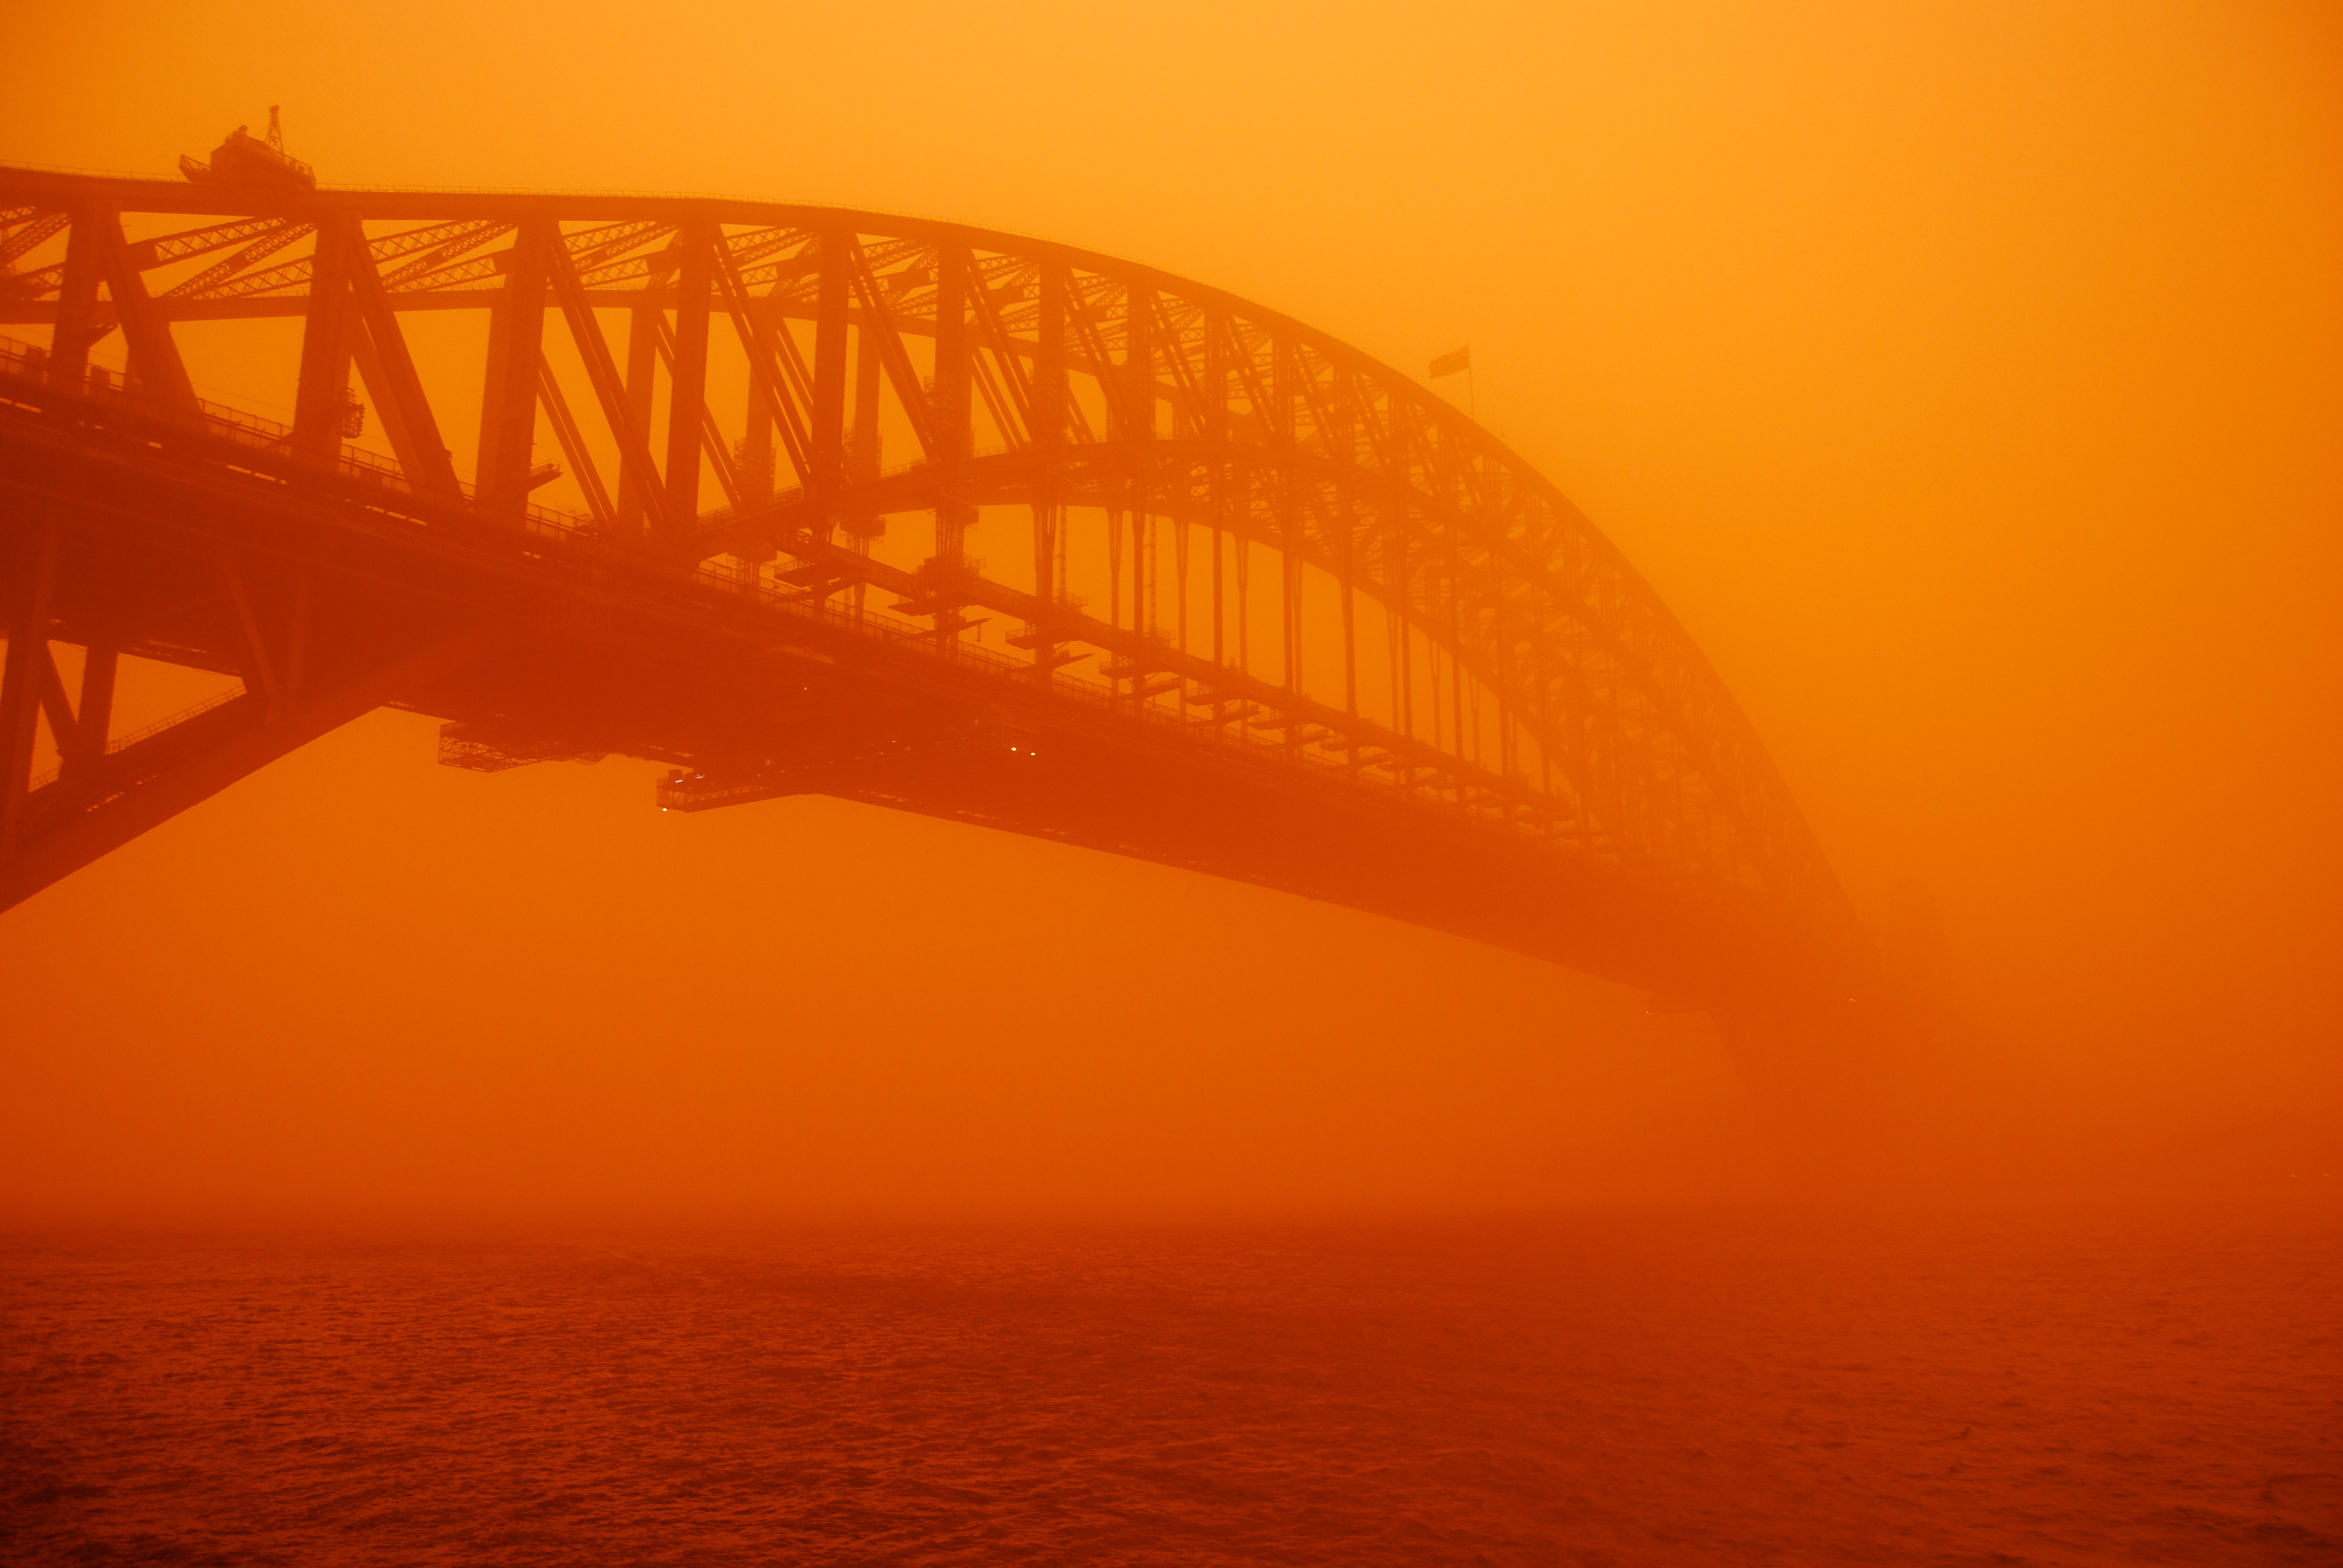
\includegraphics[width=\textwidth]{bilder/reddawn/SHB.jpg}
	\end{minipage}\hfill
	\begin{minipage}[c]{0.49\textwidth}
		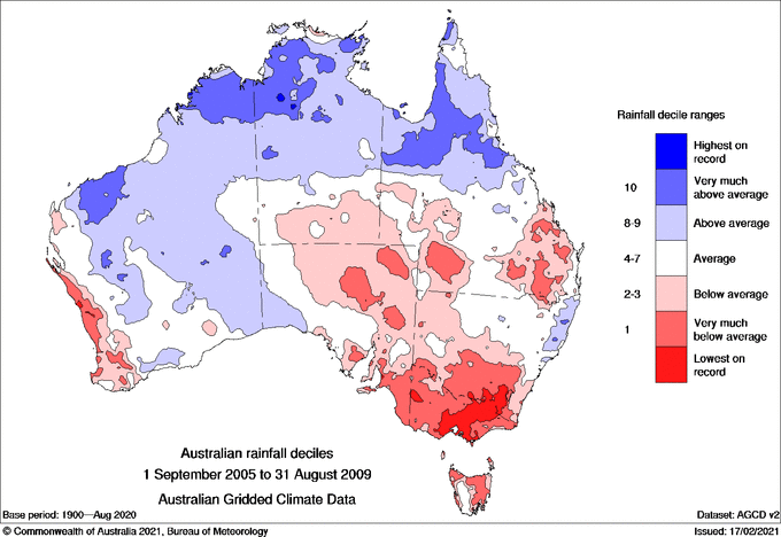
\includegraphics[width=\textwidth]{bilder/reddawn/drought.png}
	\end{minipage}\hfill
	\caption{Links: Aufnahme der Sydney Harbour Bridge während des Red Dawn Events (https://en.wikipedia.org/wiki/2009_Australian_dust_storm). Rechts: Regenfälle in Dezile für die letzten 4 Jahre vor Red Dawn. Dunkelrot: 90 \% der Vergleichszeiträume hatten mehr Regen in dieser Region, dunkelblau: 90 \% der Vergleichszeiträume hatten weniger Regen.} \label{fig:reddawn}
\end{figure}
Dieses Klima bot entsprechend günstige Bedingungen für die Entstehung eines Staubsturms. Auf Abbildung \ref{fig:bom_analysis} ist das Tiefdruckgebiet dargestellt, welches mit den starken Emissionen in Verbindung gebracht wird. Einen Tag vor dem eigentlichen Ereignis befindet es sich direkt südlich von Südaustralien, bereits losgelöst von der südlichen Polarfront. Aus diesem und der zugehörigen Kaltfront (blau) resultieren Winde in Sturmstärke (sh. Abb. \ref{fig:wind_reddawn}), die den Staub letztendlich in die Atmosphäre abtragen insbesondere in östliche Richtung weitertransportieren \citep{Leys.2011}.\citet{Leys.2011} schätzen, dass 2.54 Tg Staub über die Küste hinaus transportiert wurden.  Es wurden verschiedene Quellen identifiziert, welche im Rahmen des Ereignisses Staub emittiert haben sollen:
\begin{itemize}
\item Unteres Lake Eyre Becken in Südaustralien (\cite{Leys.2011}, \cite{Leys.2009}) (Für Canberra-Staub: Lake Torrins gem. \cite{Deckker.2014})
\item Bergbaugebiete um Cobar und Broken Hill  (\cite{Leys.2011})
\item Weideland im Nordwesten von New South Wales (\cite{Leys.2011}, \cite{Leys.2009})
\item Channel Country in Queensland (\cite{Leys.2011},\cite{Leys.2009})
\end{itemize}
\citet{Leys.2011} folgern, dass neben den Seen und Flusslandschaften als übliche Quellen insbesondere Weideland und Sandflächen Staub emittiert und letztlich zu der bemerkenswerten rötlichen Färbung geführt haben.
\begin{figure}
	\begin{minipage}[c]{0.33\textwidth}
		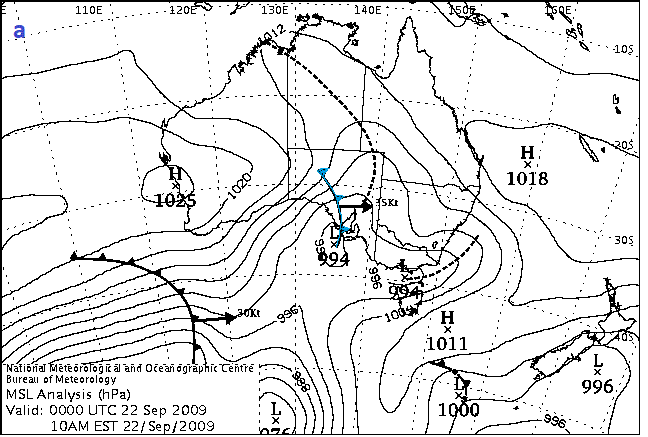
\includegraphics[width=\textwidth]{bilder/reddawn/2009092200.png}
	\end{minipage}\hfill
	\begin{minipage}[c]{0.33\textwidth}
		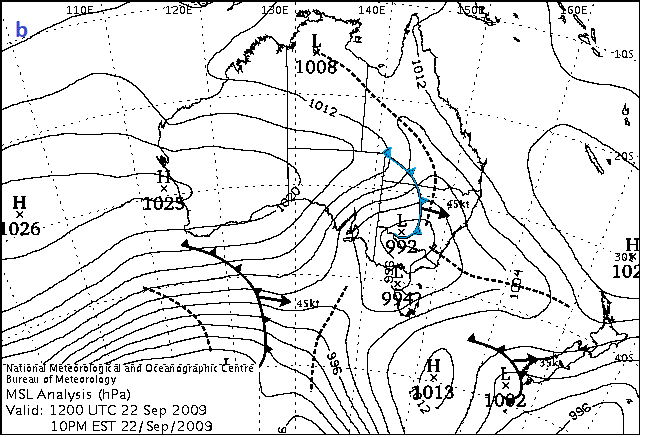
\includegraphics[width=\textwidth]{bilder/reddawn/2009092212.png}
	\end{minipage}\hfill
		\begin{minipage}[c]{0.33\textwidth}
		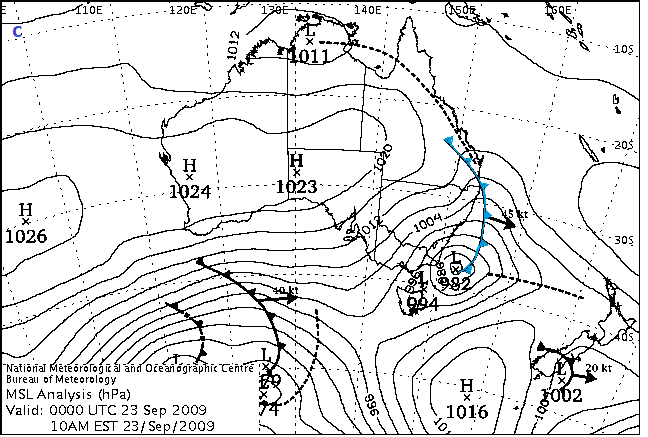
\includegraphics[width=\textwidth]{bilder/reddawn/2009092300.png}
	\end{minipage}\hfill
	\caption{Bodendruck und Fronten-Analysen des australischen Bureau of Meteorology für a) den 22.09.2009 um 0 Uhr UTC, b) später um 12 Uhr UTC und c) der 23.09.2009 wieder um 0 Uhr UTC. Die Kaltfront, die mutmaßlich für die starken Staubemissionen bzw. den sogenannten \textit{Red Dawn} in Sydney geführt hat, wurde nachträglich blau gekennzeichnet.} \label{fig:bom_analysis}
\end{figure}
\begin{figure}
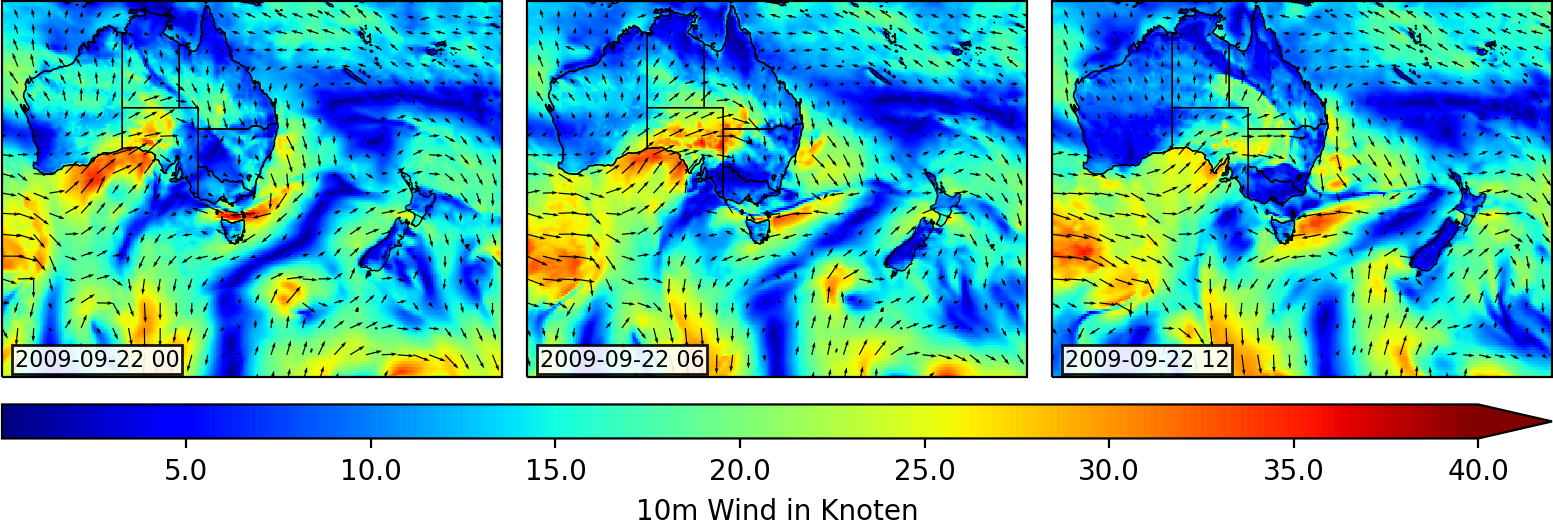
\includegraphics[width=\textwidth]{bilder/reddawn/wind_reddawn_small.png}
\caption{Windgeschwindigkeiten zu den Zeitpunkten der Staubemissionen vom 22.09. 0 Uhr UTC bis 12 Uhr UTC. Im südlichen Lake Eyre Becken erreicht der Wind gegen 6 Uhr UTC Sturmstärke.} \label{fig:wind_reddawn}
\end{figure}
\begin{figure}
	\begin{minipage}[c]{0.33\textwidth}
		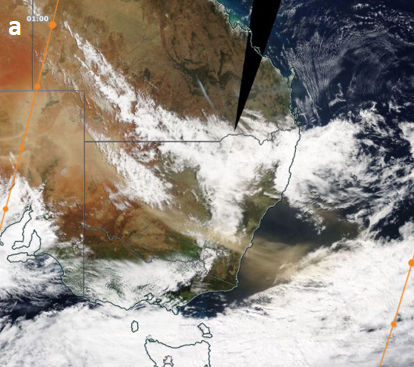
\includegraphics[width=\textwidth]{bilder/reddawn/2209T01.png}
	\end{minipage}\hfill
		\begin{minipage}[c]{0.329\textwidth}
		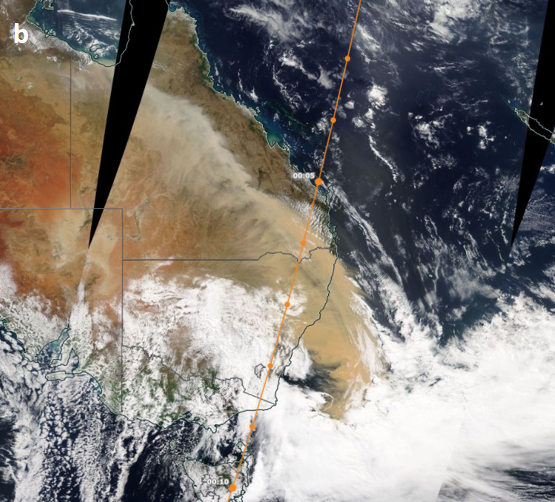
\includegraphics[width=\textwidth]{bilder/reddawn/2309T00.png}
	\end{minipage}\hfill
		\begin{minipage}[c]{0.32\textwidth}
		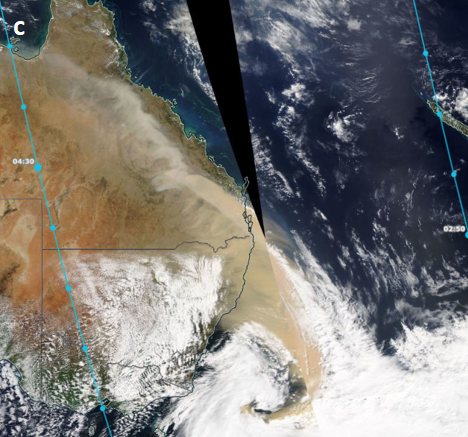
\includegraphics[width=\textwidth]{bilder/reddawn/2309T04.png}
	\end{minipage}\hfill
		\begin{minipage}[c]{0.33\textwidth}
		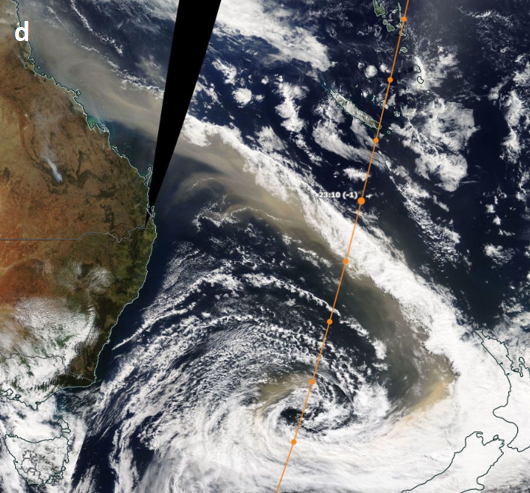
\includegraphics[width=\textwidth]{bilder/reddawn/2409T00.png}
	\end{minipage}\hfill		
	\begin{minipage}[c]{0.33\textwidth}
		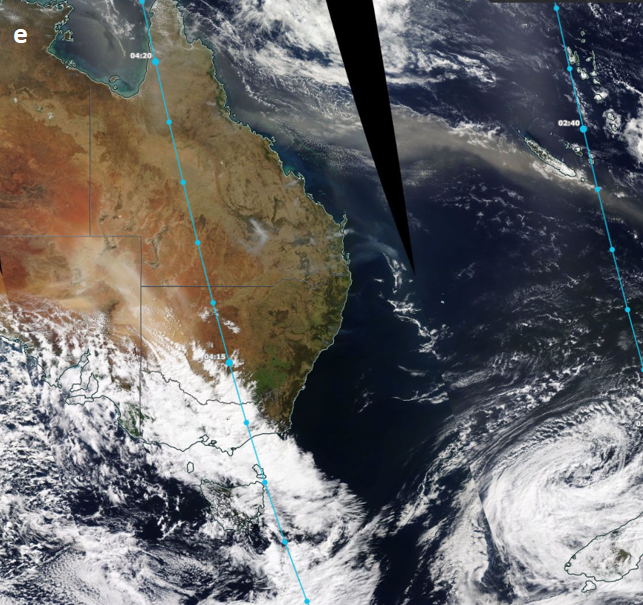
\includegraphics[width=\textwidth]{bilder/reddawn/2509T04.png}
	\end{minipage}\hfill
		\begin{minipage}[c]{0.32\textwidth}
		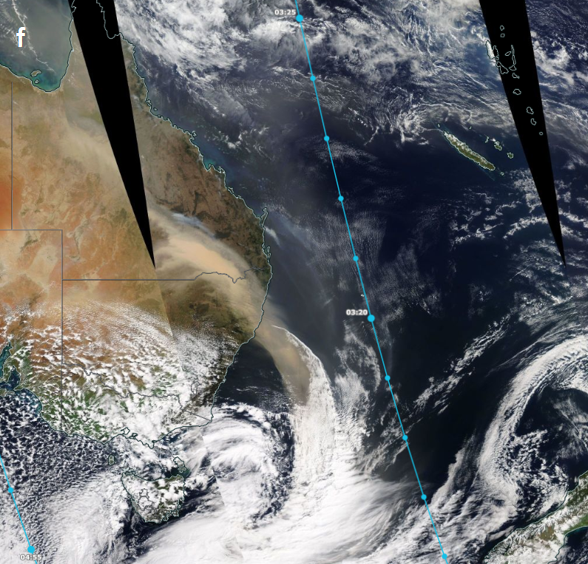
\includegraphics[width=\textwidth]{bilder/reddawn/2609T03.png}
	\end{minipage}\hfill
\caption{Aufnahmen der Satelliten AQUA und TERRA des östlichen Teils des australischen Kontinents während der Staubereignisse. a) Noch vor dem eigentlichen Red Dawn Event am 22.09. um ca. 1 Uhr UTC, b) Staubwolke mit maximaler Intensität zum Red Dawn am 23.09. um etwa 0 Uhr UTC, c) ca. 4 Stunden später mit ähnlicher Ausdehnung, d) Staubwolke deutlich im Einfluss des Tiefdruckgebiets am 24.09. um 0 Uhr UTC, e) Staub verteilt in der Atmosphäre am 25.09. um ca. 4 Uhr UTC und f) das nächste Ereignis verbunden mit neuen Emissionen am 26.09. um ca. 3 Uhr UTC.  Screenshots aufgenommen aus NASA Worldview (https://worldview.earthdata.nasa.gov/).} \label{fig:satellite}
\end{figure}
Mit dem Ereignis geht mäßiger bis moderater Niederschlag einher (sh. Abb.  \ref{fig:rain}). Dieser fällt im Süden von New South Wales und mit einem Maximum über dem tasmanischen Meer. Regen führt zu nassem Eintrag bzw. \textit{Auswaschen} des Staubs, was insbesondere für die Löslichkeit des eingebrachten Staubs eine entscheidene Rolle spielen kann \citep{Gabric.2016}. 
\begin{figure}
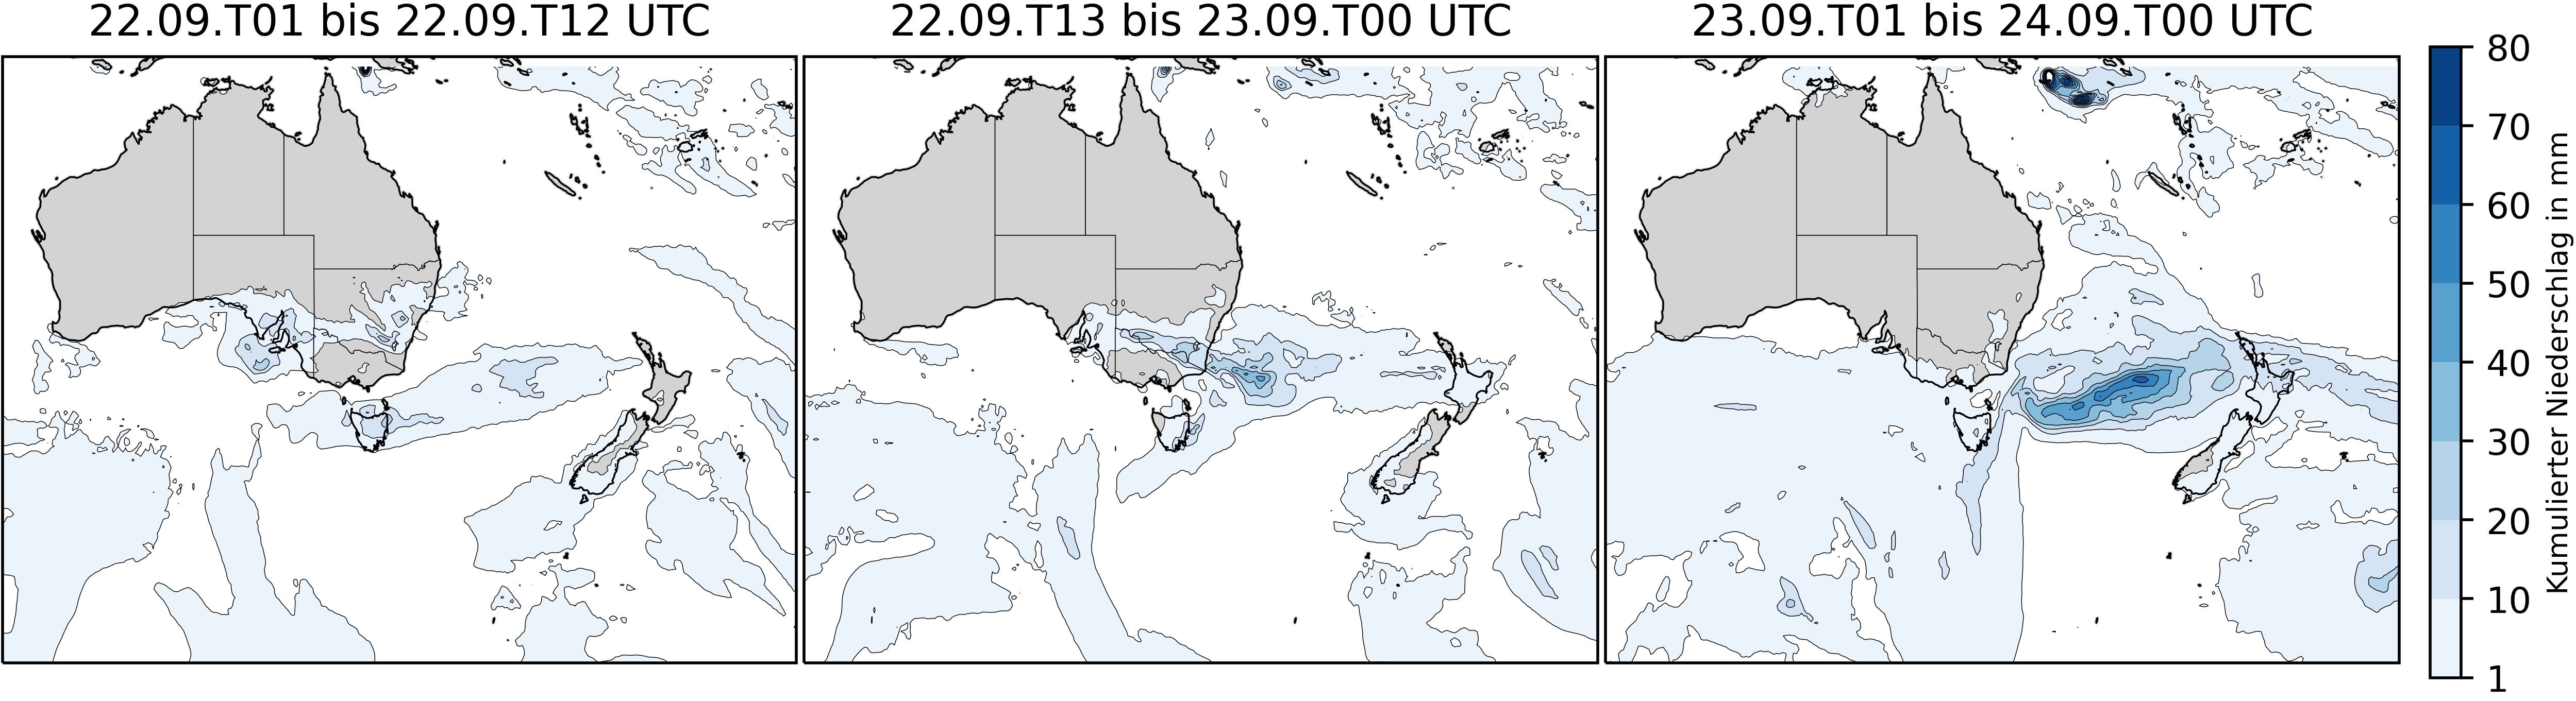
\includegraphics[width=\textwidth]{bilder/reddawn/rain.png}
\caption{Kumulierter Niederschlag im Zusammenhang mit \textit{Red Dawn} bzw. dem assozierten Tiefdruckgebiet mit der Kaltfront. Aus dem Reanalyse-Datensatz \textit{ERA5 hourly data on single levels from 1979 to present}, zur Verfügung gestellt über den Copernicus Climate Data Store (DOI: 10.24381/cds.adbb2d47) } \label{fig:rain}
\end{figure}
\section{Methoden und Daten} \label{sec:Methoden}
Um testen zu können, ob ein extremes Staubereignis Auswirkungen auf die Phytoplanktonproduktion in einer bestimmten Region hat, ist eine geeignete Datenbasis erforderlich. Grundsätzlich müssen hierzu zwei Variablen räumlich und zeitlich quantifiziert werden: Staub- und Phytoplankton-Konzentrationen. In beiden Fällen ist die Auflösung in jeder dieser Dimensionen stark beschränkt. Speziell Ausdehnung und Trajektorien von Staubstürmen müssen aufgrund der spärlichen Beobachtungsdaten (siehe Kapitel  \ref{sec:reddawn}) größtenteils geschätzt werden. Simulationen leistungsfähiger Modelle können die Auswertungen deutlich verbessern. In Rahmen dieser Arbeit wird eine spezielle WRF-Simulation (sh. Kapitel \ref{sec:wrf}) verwendet, um genauere Aussagen über das Verhalten der Staubwolke treffen zu können. Die Konzentrationen des Phytoplanktons werden (wie üblich) aus satellitengestützten täglichen Messungen der Chlorophyll a Konzentrationen abgeleitet (sh. Kapitel \ref{sec:chla}). Für den finalen Test eines möglichen Zusammenhangs werden die in Kapitel \ref{sec:stats} vorgestellten statistischen Methoden angewendet.

\subsection{WRF Modell} \label{sec:wrf}
Das \textit{Weather Research and Forecasting} (WRF) Modell ist ein mesoskaliges System zur numerischen Wettersimulation. Es findet in der Atmosphärenforschung breite Anwendung und kann für verschiedene Zwecke mit Auflösungen von weniger als einem Meter bis hin zu mehreren tausend Kilometern eingesetzt werden \citep{NCAR.2021}. Das ursprüngliche Modelle wurde um ein Modul ergänzt, dass neben den \textit{üblichen} meteorologischen Größen auch Staub-Emission, -Transport und -Deposition berücksichtigt. Im Rahmen dieser Arbeit wird der Output eines WRF-Modells der Version 4.1.2 verwendet, welcher zusätzlich die modellierten Konzentrationen des Elements Eisen enthält. Als Staub-Emissionsschema wurde jenes von \citet{Shao.2004} verwendet. Das Modell berechnet die Staubkonzentrationen für 5 verschiedene Korngrößenklassen, welche in Tabelle \ref{table:wrf} dargestellt sind. Simuliert wurde der Zeitraum vom 18.09.2009 um 0 Uhr UTC bis zum 30.09.2009 um 0 Uhr UTC. Die verfügbaren Variablen werden in der Ausgabedatei in einem Intervall von drei Stunden gespeichert, wodurch sich insgesamt 97 auswertbare Zeitschritte ergeben. Zum Startzeitpunkt werden dem Modell keine atmosphärischen Staubkonzentrationen übergeben. Etwaige Emissionen zu früheren Zeitpunkten werden demnach vernachlässigt. Räumlich deckt das Modell von 110.3° Ost bis 170.3° West und von 57.06° S bis 9.89° S den gesamten australischen Kontinent, das tasmanische Meer, Neuseeland und Teile des südlichen Ozeans und Pazifiks ab. Dieses Gebiet wird mit 164$\times$124 (Ost-West$\times$Süd-Nord) Gitterpunkten abgedeckt. Ein Gitterpunkt repräsentiert damit ein Gebiet von etwa 53.3 km$\times$29.5 km (am nördlichsten Punkt in der Domäne, im Süden sind es 29.4 km$\times$53.3 km). Mehrere Größen, die für Emission, Transport und Deposition wichtig sind (bspw. lokale Form des Geländes, steile Topographie, Rauheit, Turbulenzen), können nicht aufgelöst werden und müssen im Modell parametrisiert werden. Die vertikale Verteilung wird auf 32 Höhenlevel simuliert. Das unterste Höhenlevel ist (entsprechend der Auflösung) geländefolgend, das oberste liegt oberhalb der Troposphäre zwischen 19.044 m und 20.230 m über Meeresniveau.
\begin{table}[H]
\begin{tabularx}{0.3\textwidth}{X X}
		\toprule
			\thead{Größenklasse} & \thead{Effektiver Radius}\\
		\midrule
		1 & $0.5 \ \mu$m \\
		2 & $1.4 \ \mu$m \\
		3 & $2.4 \ \mu$m  \\
		4 & $4.5 \ \mu$m \\
		5 & $8.0 \ \mu$m  \\
		\bottomrule
\end{tabularx}
\caption{Die Staubpartikel wurden in verschiedene Korngrößen unterteilt} \label{table:wrf}
\end{table}
\subsubsection{Emissions Schema}
Zur Modellierung der Staubemissionen wurde das Schema von \citet{Shao.2004} verwendet und in WRF implementiert. Als Auslöser für Emissionen werden grundsätzlich zwei Mechanismen erwogen: Beschuss durch Salz und der Zerfall von Aggregaten. Zusammengefasst setzt sich das Emissionsschema \citep{Shao.2004} aus folgenden Gleichungen zusammen:
\begin{align}
\tilde{F} (d_i,d_s) &= c_y \eta_{fi} \left[\left(1-\gamma\right) + \gamma
\sigma_p \right] \left(1+\sigma_m \right) \frac{g \cdot Q}{u^2_*} \\
\gamma &= \exp \left[-\left(u_* - u_{*t} \right)^3\right] \\
\sigma_m &= 12 \cdot u_*^2 \frac{\rho_b}{p} \left(1 +14 \cdot u_* \sqrt{\frac{\rho_b}{p}} \right)
\end{align}
Dabei ist $\tilde{F}(d_i,d_s)$ die Emissionsrate für die Staubpartikelgröße $d_i$ und das Salz der Partikelgröße $d_s$; $c_y$ ein dimensionsloser Koeffizient; $\eta_{fi}$ der Anteil des insgesamt emittierbaren Staubs; $\sigma_p = \frac{\eta_{mi}}{\eta_{fi}} = \frac{p_{m}(d_i)}{p_{f}(d_i)}$ das Verhältnis zwischen der Massenverteilung freien Staubs $\eta_{mi}$ zu der des ingesamt emissionsfähigen Staubs $\eta_{fi}$ pro Einheitsbodenmasse für die Partikelgrößenklasse $i$ bzw. den entsprechenden Verteilungen für die Partikelgrößenverteilungen $p_{m}(d_i)$ und $p_{f}(d_i)$;  $\sigma_m= \frac{m_\Omega}{m}$ das Verhältnis zwischen der Masse  $m$ des einschlagenden Partikels und der durch \textit{Bombardement} ausgeworfenen Masse $m_\Omega$; $g$ die Erdschwerebeschleunigung; $Q$ der stromweise Salzfluss; $u_*^2$ die Reibungsgeschwindigkeit; $u_{*t}^2$ der Schwellenwert für die Reibungsgeschwindigkeit; $\rho_b$ die Bodenschüttdichte und $p$ der plastische Bodendruck.
\subsection{Chlorophyll a} \label{sec:chla}
Um die Taxonomie und die genauen Konzentrationen des Phytoplanktons im Meerwasser abzuleiten, sind in situ Messungen erforderlich. Für die Untersuchung eines Zusammenhangs in dieser Arbeit ist es allerdings ausreichend, die grundsätzliche Tendenz der Entwicklung der Phytoplankton Konzentrationen zu quantifizieren. Eine explizite Kenntnis der speziellen Zusammensetzung ist nicht erforderlich, kann aber anhand vorangegangener Untersuchungen und der für die jeweilige Region erwartbaren Verteilungen abgeschätzt werden. Messungen des in Pflanzen enthaltenen Farbstoffs Chlorophyll erlauben, Produktion und Konzentrationen von Phytoplankton abzuleiten \citep{RYTHER.1957}. Dementsprechend ist es zu diesem Zweck üblich, die Nettoprimärproduktion aus Satellitenbildern abzuleiten, welchen Werte des Hauptpigments \textit{Chlorophyll a} zugewiesen werden können. Da die Reaktionszeit auf möglichen \textit{Dünger} mit 4-5 Tagen (vgl. Kapitel \ref{sec:Phytobasics}) relativ kurz ist, ist es vorteilhaft, zeitlich möglichst hoch aufgelöste, tägliche Daten zu verwenden. Eine erhebliche Einschränkung dieser satellitengestützten Daten ist, dass die Beobachtungen nur über eis- und wolkenfreiem Himmel möglich sind. Zusätzlich kann reflektiertes Sonnenlicht die Ableitung erschweren. Auf Abbildung \ref{fig:chla} wird beispielhaft demonstriert, dass diese Faktoren zu einer sehr schlechten räumlichen Auflösung führen können. Glücklicherweise bietet der \textit{Copernicus Marine Service} bzw. \citet{Saulquin.2019} einen überarbeiteten Datensatz für den Betrachtungszeitraum, welcher die fehlenden Beobachtungsdaten mithilfe aktueller Algorithmen in täglicher Auflösung interpoliert. Obwohl dieser Datensatz die gewässertypischen Besonderheiten berücksichtigt und auf Basis fundierter Interpolationsmethoden zusammengestellt wurde, muss aufgrund der schlechten Abdeckung (insbesondere mit zunehmender geographischer Breite) bei der späteren Interpretation ein entsprechend hoher möglicher Fehler beachtet werden. Die Werte werden  aus den Messungen mehrerer Sensoren/Spektrometer (MERIS, MODIS und SeaWiFS) zusammengestellt. Mithilfe Temperatur des Oberflächenwassers, einfallender Sonnenstrahlung, mixed-layer-depth, Up- und Downwellingzonen kann aus CHL-a Konzentration die NPP abgeleitet werden \citep{Falkowski.1998}.

\begin{figure}
	\begin{minipage}[c]{0.49\textwidth}
		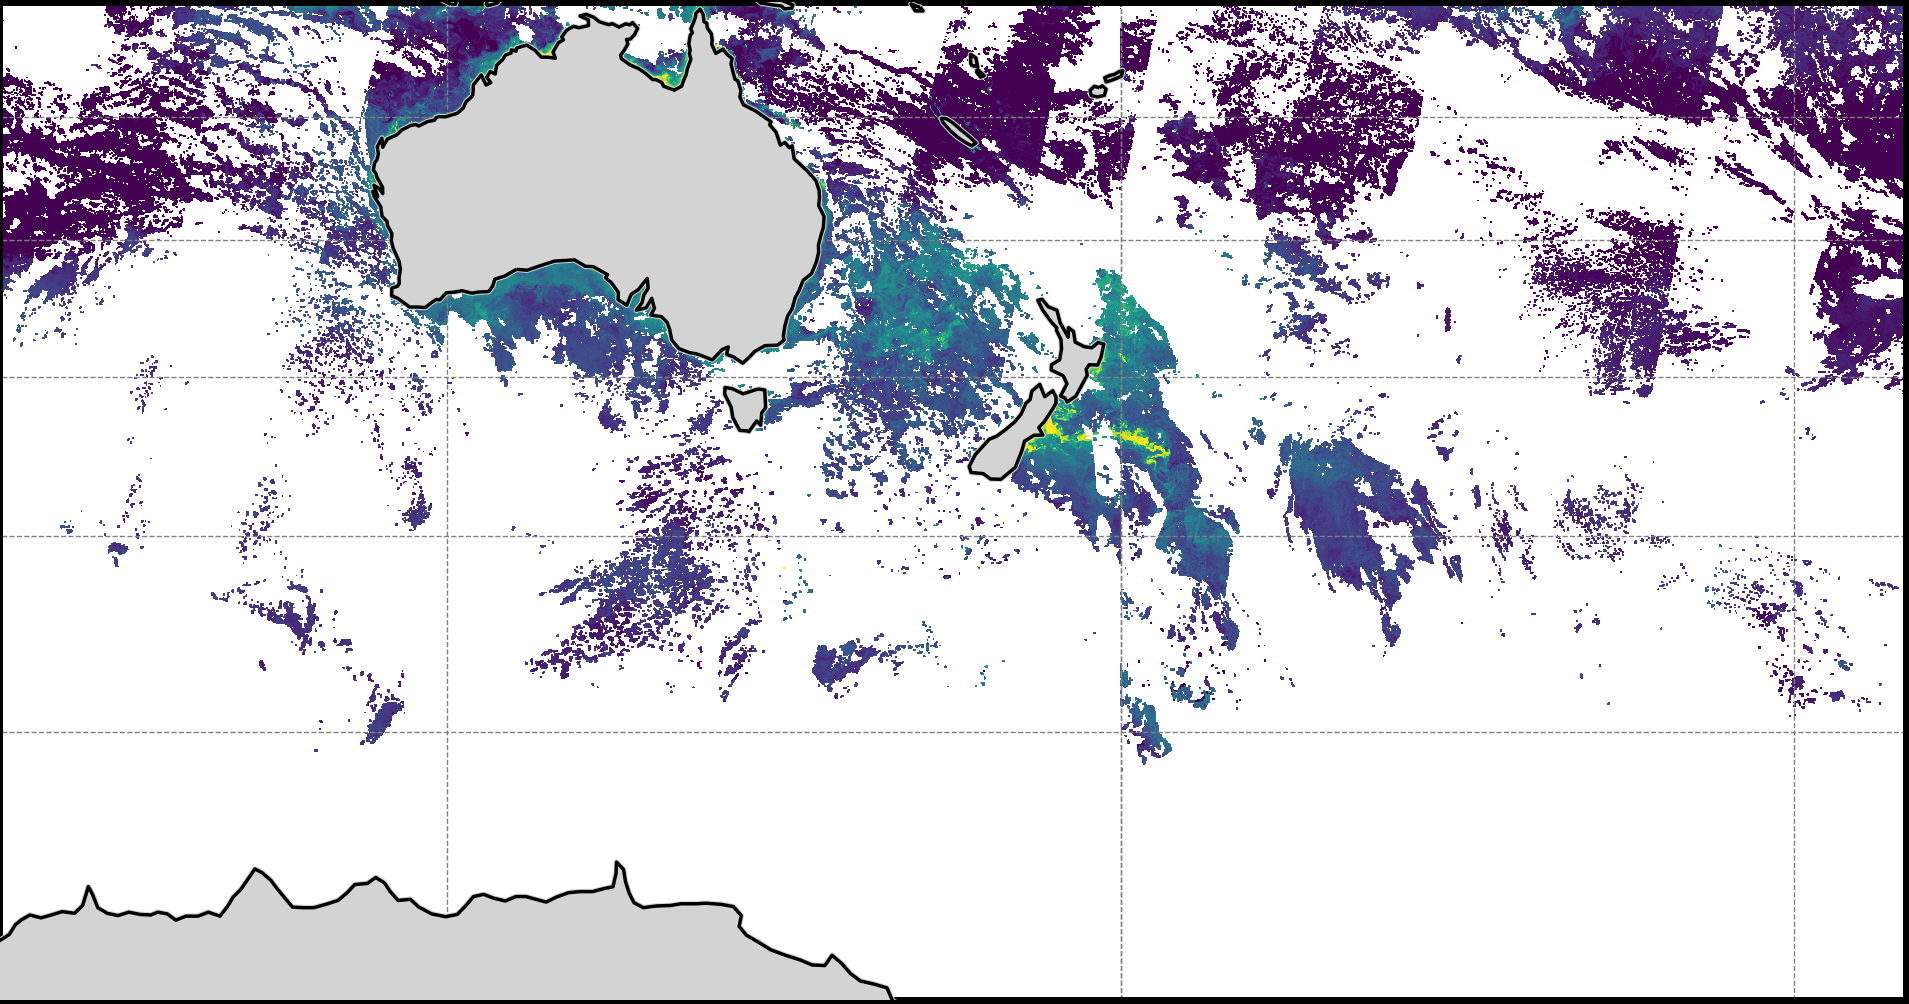
\includegraphics[width=\textwidth]{bilder/chla_raw.png}
	\end{minipage}\hfill
	\begin{minipage}[c]{0.49\textwidth}
		 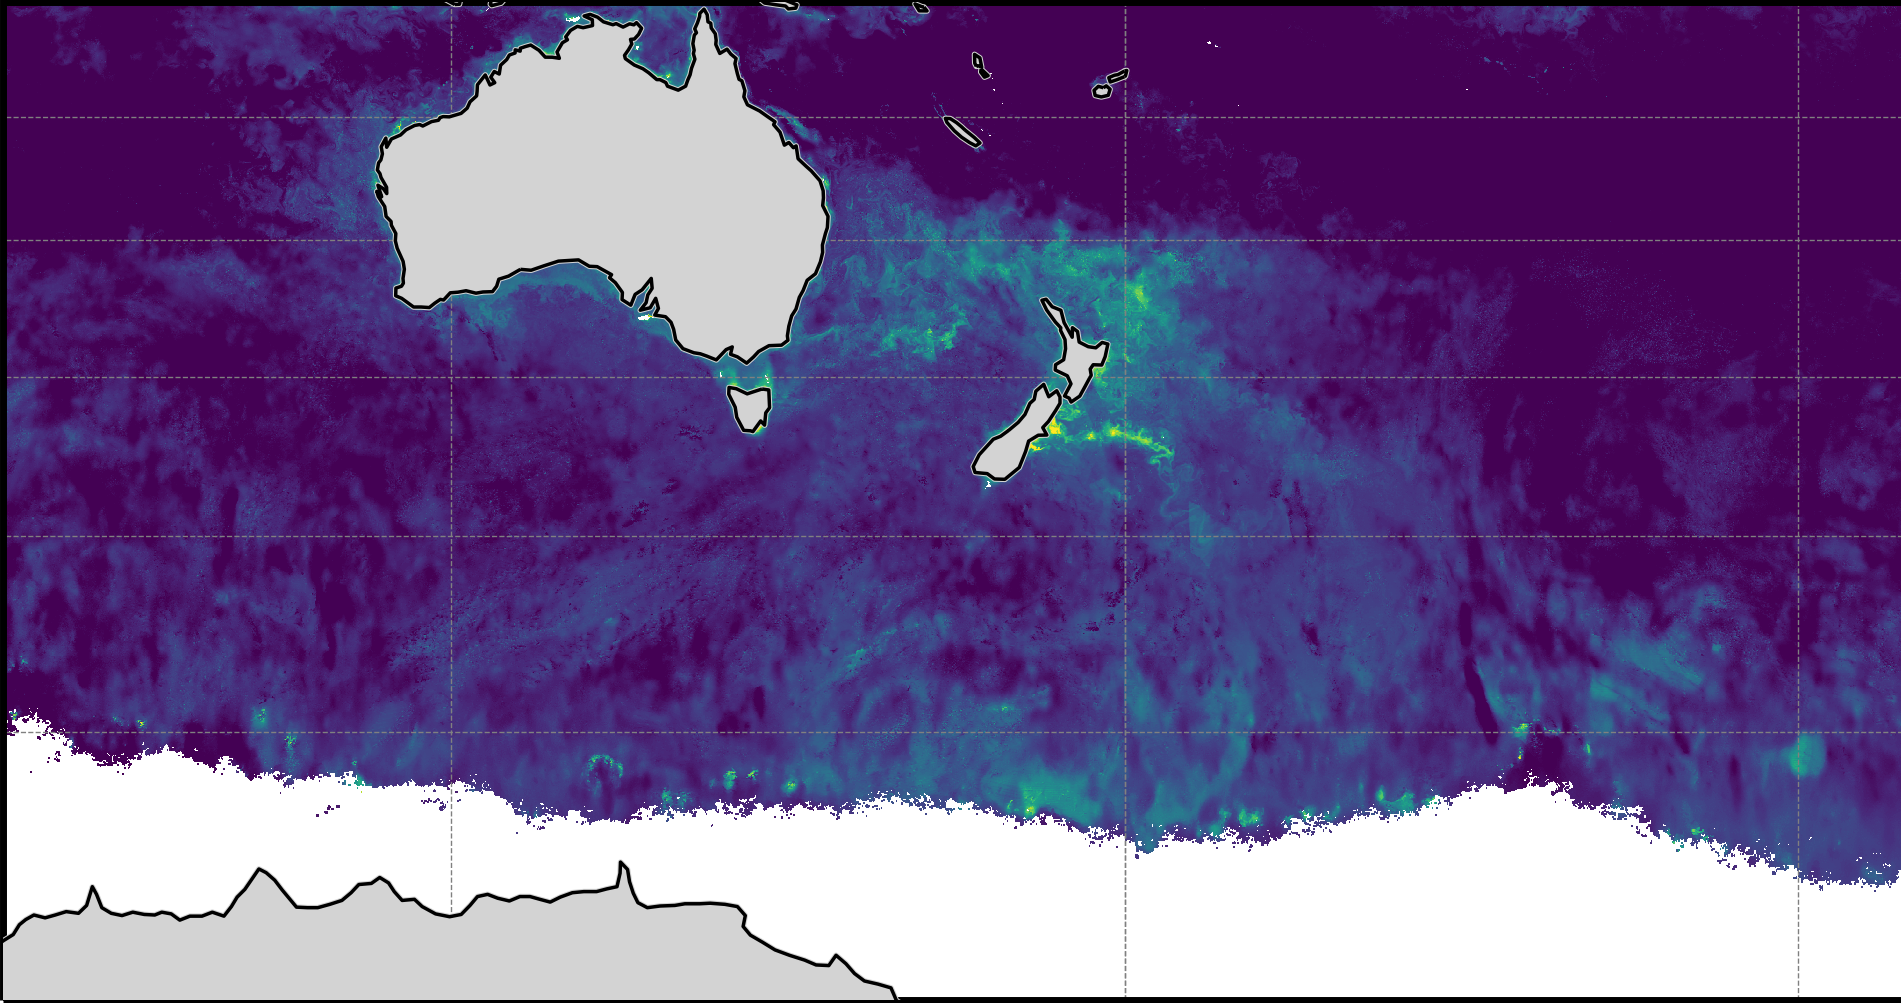
\includegraphics[width=\textwidth]{bilder/chla_interpol.png}
	\end{minipage}\hfill
	\caption{Beispielhaft die zum 01.09.2009 abgeleiteten Chlorophyll a Konzentrationen. Links: Ableitung auf Basis der Beobachtungsdaten (Ocean colour daily data des Climate Data Store). Für alle weißen Flächen liegen keine Daten vor. Rechts: Mithilfe weiterer Algorithmen von \citet{Saulquin.2019} interpolierte Werte für eine vollständigere Abdeckung.} \label{fig:chla}
\end{figure}
\subsection{Statistische Methoden} \label{sec:stats}
Um den statistischen Zusammenhang zwischen Staub-/Eiseneintrag und Phytoplankton zu untersuchen, werden hier zwei verschiedene Verfahren angewendet. Zunächst wird anhand einer Zeitreihenanalyse der mittleren Konzentrationen des Phytoplanktons (Kapitel \ref{sec:timeseries}) überprüft, ob im Untersuchungszeitraum nach dem Staubsturm  anschaulich eine Veränderung beobachtet wird. 
\subsubsection{Zeitreihen- und Trendanalyse} \label{sec:timeseries}
Für die Zeitreihenanalyse werden alle Gitterzellen betrachtet, für die von der WRF-Simulation ausreichend hohe Eisendepositionen simuliert wurden. Um das Gebiet sinnvoll einzugrenzen, soll der gesamte Eintrag für die jeweilige relevante Zelle so groß sein, dass dadurch die \textit{normalen} Eisenkonzentrationen nennenswert erhöht werden. Auf Basis von Abbildung \ref{fig:nutrient_iron} wird angenommen, dass diese \textit{normalen Konzentrationen} für den überwiegenden Teil der zu untersuchenden Region mindestens etwa 0.066 nM (Nanomol pro Liter) betragen. Darüber hinaus wird zur Abschätzung der Erhöhung der Eisenkonzentrationen $C_\text{Fe}$ durch die Staubereignisse angenommen, dass der überwiegende Teil der Nährstoffe in den oberen $z_0 = 10$m des Oberflächenwassers konsumiert wird. Mit  $M_{\text{Fe}} =  55.845$ g/mol Molmasse des Elements Eisen ergibt sich die vom Modell simulierte totale Eisendeposition $m_\text{Fe}$ pro Einheitsfläche $A=1$ Quadratmeter durch Integration des Eisenflusses $F_\text{Fe}$ über die Gesamtsimulationszeit:
\begin{equation}
\frac{m_\text{Fe}}{A} = \int F_\text{Fe} \cdot dt
\end{equation}
Bei Vernachlässigung des Flusses (Zu-/Abtransport) durch die oberen $z_0=10$m ergibt sich dann eine Eisenkonzentration von
\begin{equation}
C_\text{Fe} = \frac{m_\text{Fe}}{z_0 \cdot M_{\text{Fe}} \cdot A} \Leftrightarrow m_\text{Fe} = C_\text{Fe} \cdot z_0 \cdot M_{\text{Fe}}
\end{equation}
Um eine Erhöhung der Konzentrationen in der Größenordnung von $C_\text{Fe}=$0.01 nM zu erreichen, müssen dementsprechend wenigstens etwa $5.6$ µg Eisen pro Quadratmeter eingetragen werden. Zum Vergleich: In den \textit{Bottle Experiments} von \citet{Martin.1988} wurden in verschiedenen Behältern 1 nM, 5 nM und 10 nM hinzugefügt. Die Mengen waren dort also um mindestens zwei Größenordnungen höher als in dieser Annahme. Im SOIREE-Experiment für den südlichen Ozean \citep{Trull.2001} konnten Veränderungen ab einer Schwelle von etwa 0.2 nM Eisen beobachtet werden, was einer Verdopplung der dortigen regulären Konzentration von 0.1 nM entspricht \citep{Boyd.2010}. Auch im Vergleich dazu ist der hier verwendete Schwellenwert eher optimistisch, da heißt, die Depositionen reichen möglicherweise nicht aus, um eine Reaktion des Phytoplanktons zu bewirken. \\
Da die chemischen Zusammensetzungen und Bedingungen für die Regionen unterschiedlich sein können (QUELLE ERGÄNZEN), sollen die anhand des Schwellenwertes identifizierten Zellen in verschiedene Sektoren eingruppiert werden, um diese jeweils separat zu analysieren. Für jeden Sektor wird anschließend für jeden verfügbaren Zeitpunkt der Mittelwert der Chlorophyll-a-Konzentrationen $\text{C}_i$ aus den $N$ dort betroffenen Zellen berechnet. Damit ergibt sich eine Zeitreihe für die durchschnittliche Entwicklung des Phytoplanktons im gesamten Sektor $\mu(t)$:
\begin{equation}
\mu_C(t) = \frac{1}{N}\sum\limits_{i,j=1}^{N} \text{C}_{i,j}(t)
\end{equation}
Unter der Annahme, dass der Eintrag von Eisen einen Einfluss auf diese Zeitreihe nimmt, sollte diese nach dem Ereignis ansteigen. Allerdings unterliegt die Entwicklung der Phytoplankton-Konzentrationen ohnehin (so auch im tasmanischen Meer \citep{Tilburg.2002}) einem jahreszeitlichen Gang sowie weiteren externen Einflüssen, die eine hohe Variabilität aufweisen können (vgl. Kapitel \ref{sec:nährstoffe}). Da der jahreszeitliche Trend aus den Klimadaten relativ gut bekannt ist, kann die Zeitreihe im Untersuchungszeitraum 2009 um diesen Effekt bereinigt werden. Hierzu werden Datensätze des \textit{Marine Copernicus Service} verwendet, welche die nötigen täglichen Klimadaten bereits liefern. Neben dem Mittelwert der Chlorophyll-a-Konzentrationen des jeweiligen Tages für die Jahre 1998 bis 2018 kann außerdem aus der Standardabweichung und den 3\% und 97\% Perzentilen ($\sigma$,$q_{0.03}$,$q_{0.97}$,) die entsprechende Variabilität abgeleitet werden. Der Klima-Mittelwert $\text{C}_{cli,i}$ eines jeden Gitterpunktes wird ebenfalls über den gesamten jeweiligen Sektor gemittelt:
\begin{equation}
\mu_{C[cli]}(t) = \frac{1}{N}\sum\limits_{i,j=1}^{N} \text{C}_{i,j[cli]}(t)
\end{equation}
Dieser dient zur Entfernung eines möglichen Trends im zu untersuchenden Sektor, sodass ausschließlich die Abweichung/Anomalie $\Delta \mu(t)$ zum Klimamittel dargestellt wird:
\begin{equation}
\Delta \mu_C(t) = \mu_C(t) - \mu_{C[cli]}(t) \label{eq:cli_anomalie}
\end{equation} 
Im Fall eines \textit{düngenden} Effektes der Eisendpositionen sollte diese bereinigte Zeitreihe nach den Depositionen einen steigenden Trend aufweisen. Um einzuschätzen, ob die Abweichungen überhaupt relevant sind, werden diese mit der Standardabweichung sowie den 3\% und 97\% Perzentilen verglichen. Liegt die Anomalie unter der durch die Standardabweichung gegebenen Schwelle, ist ein Zusammenhang eher unwahrscheinlich, die Abweichungen könnten aus der gewöhnlichen, Staub-unabhängigen Variabilität resultieren. Liegen diese im Gegensatz deutlich darüber oder erreichen sogar das 97 \% Perzentil, handelt es sich um sehr seltene Ereignisse (in 97\% der Fälle liegen die Konzentrationen/Abweichungen) unter diesem Wert), bei denen ein externer Einfluss wahrscheinlich ist. Kann dieser in unserem Fall in einen zeitlichen Zusammenhang mit den Staubeinträgen gebracht werden, wäre das ein deutlichen Indiz für einen Einfluss ebendieser. Sämtliche Werte des Klimadatensatzes liegen je Gitterzelle vor und es werden entsprechend für den jeweiligen Sektor die Mittelwerte $\mu_\sigma (t)$, $\mu_{q_{0.03}}(t)$, $\mu_{q_{0.97}}(t)$ gebildet. $\mu_{\Delta C}(t)$ ist der Mittelwert des für jeden Gitterpunkt geschätzten Fehlers $ \Delta C_i(t)$ der abgeleiteten Chlorophyll-a-Konzentrationen $C_i(t)$ (in 2009).
\begin{figure}
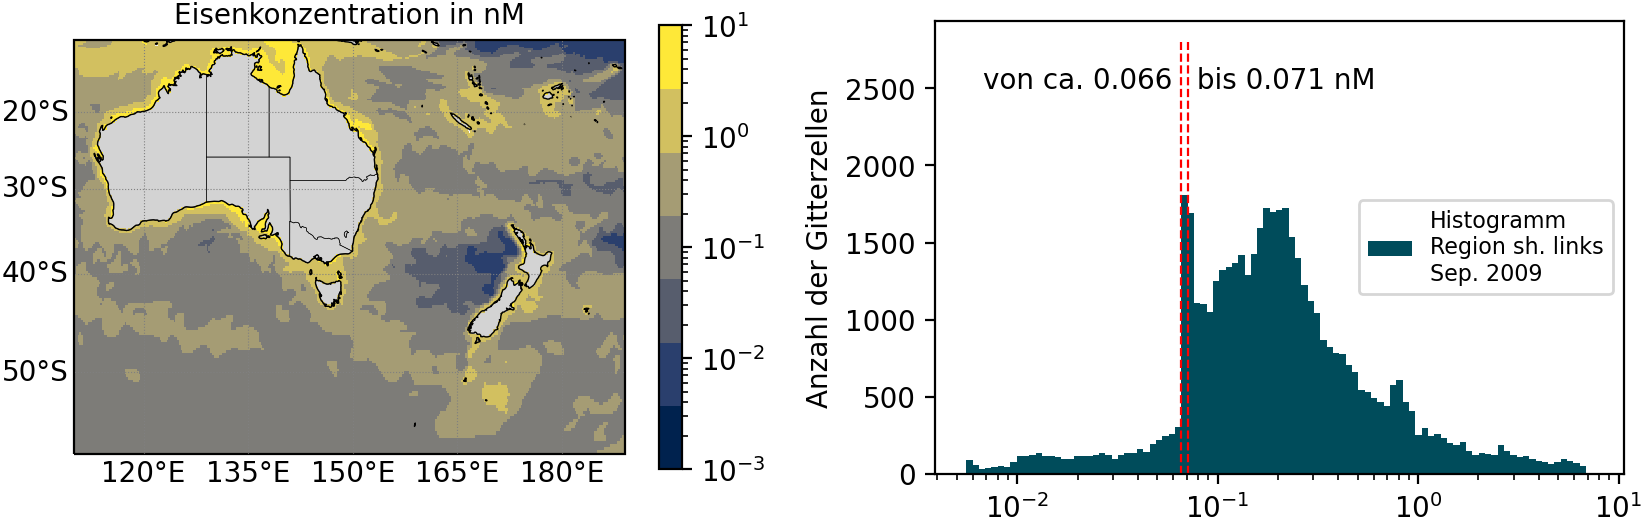
\includegraphics[width=\textwidth]{bilder/nutrient_iron.png}
\caption{Links: Die abgeleiteten Eisenkonzentrationen in der zu untersuchenden Region. Rechts: Histogramm für die Konzentrationen in den Gitterzellen. Erstellt aus dem Datensatz des Copernicus Marine Data Store, für weitere Informationen siehe https://resources.marine.copernicus.eu/documents/PUM/CMEMS-GLO-PUM-001-029.pdf} \label{fig:nutrient_iron}
\end{figure}

\subsubsection{Eisentransport durch Advektionsgleichung} \label{sec:methods_advection}
Da dank der WRF-Simulation und den gemäß \citet{Saulquin.2019} interpolierten Chlorophyll-a-Konzentrationen für die komplette Region räumlich vollständige Daten vorliegen, können diese Variablen zusätzlich zum zeitlichem Zusammenhang auch hinsichtlich etwaiger räumlicher Muster untersucht werden. Im einfachsten Fall würden exakt die Regionen mit erhöhten Chlorophyll-Konzentrationen reagieren, in denen vorher Eisen eingetragen wurde. Im Rahmen dieser Arbeit wird vereinfacht angenommen, dass die Eisenpartikel ausreichend lange im Oberflächenwasser verweilen (sh. auch \citet{Cropp.2013}), also nicht absinken und der Staubsturm grundsätzlich die einzige Eisenquelle bietet. Auch die weiteren (Wachstum-)begünstigenden oder abschwächenden Faktoren (Verfügbarkeit weiterer Nährstoffe, Wassertemperaturen, auf- und abströmen in (anti-)zyklonalen Wirbeln etc., Diffusion) werden mathematisch nicht berücksichtigt. Nichtsdestotrotz kann der laterale Transport des eingetragenen Eisens berücksichtigt werden. Die Eisenkonzentrationen $C_\text{Fe}$ an einem Ort können sich demnach gemäß der Kontinuitätsgleichung (\ref{eq:fe_continuity}) durch den Zu- oder Abfluss $\nabla . (C_\text{Fe} \vec{v})$ durch die Ozeanströmung $\vec{v} = (u,v,w)^T$  und dem Eintrag von eisenhaltigem Staub $F_\text{Fe}$ verändern, welcher sich in der Wassersäule der Höhe $z_0$ gleichmäßig verteilt:
\begin{equation}
\frac{\partial C_\text{Fe}}{\partial t} = - \nabla . (C_\text{Fe} \ \vec{v}) + \frac{1}{z_0 \cdot M_\text{Fe}} \cdot F_\text{Fe} \label{eq:fe_continuity}
\end{equation}
Da Ozeanwasser praktisch inkompressibel ist ($\nabla . \vec{v}=0$) und die Vertikalgeschwindigkeit $w$ vernachlässigt werden soll, reduziert sich der Ausdruck auf die zweidimensionale Advektionsgleichung:
\begin{equation}
\frac{\partial C_\text{Fe}}{\partial t} = - \vec{v} . \nabla_h  C_\text{Fe}  + \frac{1}{z_0 \cdot M_\text{Fe}} \cdot F_\text{Fe}
\end{equation}
Diese wird nach dem Upwind-Schema diskretisiert, sodass sich anschließend die Eisenkonzentrationen am Gitterpunkt $i,j$ für die Zeitschritte $n$ mit $\Delta t$= 3 Stunden ergeben:
\begin{equation}
\begin{split}
C_{i,j}^n = &\ C_{i,j}^{n-1} - u_{i,j}^{n-1} \cdot \frac{\Delta t}{\Delta x_{i,j}} \cdot (C_{i,j}^{n-1} - C_{i,j-1}^{n-1}) \\\\
&- v_{i,j}^{n-1} \cdot \frac{\Delta t}{\Delta y_{i,j}} \cdot (C_{i,j}^{n-1} - C_{i-1,j}^{n-1})  \\\\
&+ \frac{\Delta t}{z_0 \cdot M_\text{Fe}} \cdot F_\text{Fe} \text{ \qquad  \qquad \qquad für } u,v > 0 \\\\
\end{split}
\end{equation}
Die Courant-Zahl $c = u \cdot \Delta t / \Delta x$ bzw. $v \cdot \Delta t / \Delta y$ bleibt in diesem Fall bei den minimalen Gitterpunktabständen von knapp 30km (sh. Kapitel \ref{sec:wrf}) für Strömungskomponenten $u,v \ < 2.6$ (in unserem Fall überall gegeben) kleiner als 1, sodass das Schema gemäß der \textit{Courant-Friedrich-Lewy}-Bedingung stabil bleibt. Die Strömungsgeschwindigkeit auf den Landflächen beträgt Null. Als Randbedingungen können die Eisenkonzentrationen der Landflächen gleich Null oder auf einen festen Wert gesetzt werden. 
\subsubsection{Korrelationsanalyse} \label{sec:methods_correlation}
Um einen räumlichen Zusammenhang zwischen den Veränderungen der Eisenkonzentrationen $\partial C_\text{Fe} / \partial t$ und den Veränderungen in den Chlorophyll-a-Konzentrationen $\partial C / \partial t$ zu untersuchen, wird eine Korrelationsanalyse beider Zeitreihen durchgeführt. Gemäß der Kontinuitätsgleichung \ref{eq:continuity} können sich ebenso wie die Eisenkonzentrationen die Chlorophyll-a-Konzentrationen an einem Ort nur durch Zu- und/oder Abfluss und aufgrund möglicher Quellen $S_C$ ändern.
\begin{equation}
\frac{\partial C}{\partial t} = - \nabla . (C \ \vec{v}) + S_C  \overset{\text{inkompressibel}}{=} - \vec{v}.\nabla C + S_C \label{eq:continuity}
\end{equation}
Im Rahmen der Analyse wird der Fluss $\vec{v}.\nabla C$ hier jedoch vernachlässigt und die Veränderungen werden ausschließlich auf die mögliche Quelle (Wachstum nach Düngung durch zusätzlich verfügbarem Eisen) mit einer (hier unbekannten) Wachstumsfunktion $S_C = f(\partial C_\text{Fe} / \partial t)$ zurückgeführt. Falls ein (näherungsweise) linearer Zusammenhang besteht, hängt die Entwicklung der Chlorophyll-a-Konzentrationen dann direkt proportional von den verfügbaren bzw. veränderten Eisenkonzentrationen ab, sodass dieser Zusammenhang im Rahmen einer Korrelationsanalyse sichtbar werden sollte. Im ersten Schritt werden die Koordinaten (d.h. die Gitterpunkte) der Chlorophyll-a-Daten auf die des Eisenflusses aus der WRF-Simulation angepasst. Anschließend werden nach dem expliziten Euler-Rückwärts-Verfahren die Ableitungen für die täglichen Chlorophyll-a-Daten ($\Delta t = 1d$) berechnet:
\begin{equation}
\left[\frac{\partial C}{\partial t}\right]_{i,j}^{n} \approx \frac{C_{i,j}^n-C_{i,j}^{n-1}}{\Delta t}
\end{equation}
Danach werden für jeden Gitterpunkt die Kreuz-Korrelationen für verschiedene Zeit- ($\tau$ in Tagen) und Gitterpunkt- ($\Delta i$,$\Delta j \in \mathbb{Z}$) Verschiebungen bestimmt:
\begin{equation}
R_{i,j}(\tau,\Delta i, \Delta j)= \frac{1}{N_t}\sum\limits_{n=1}^{N_t} \left[\frac{\partial C_\text{Fe}}{\partial t}\right]_{i,j}^n \cdot \left[\frac{\partial C}{\partial t}\right]_{i+\Delta i ,j+\Delta j}^{n+\tau}
\end{equation}
Daraus können noch durch Subtraktion der Zeitmittelwerte die Kovarianz und der durch Normierung um die zeitlichen Standardabweichung auf das Intervall $[-1,1]$ beschränkte Korrelationskoeffizient $\rho_{i,j}(\tau,\Delta i, \Delta j)$ berechnet werden:
\begin{equation}
\text{cov}_{i,j}(\tau,\Delta i, \Delta j) = R_{i,j}(\tau,\Delta i, \Delta j)-\left[\frac{\overline{\partial C_\text{Fe}}}{\partial t}\right]_{i,j} \cdot \left[\frac{\overline{\partial C}}{\partial t}\right]_{i+\Delta i,j+\Delta j}^{+\tau}
\end{equation}
\begin{equation}
\rho_{i,j}(\tau,\Delta i, \Delta j) = \frac{\text{cov}_{i,j}(\tau,\Delta i, \Delta j)}{\sigma \left(\left[\frac{\partial C_\text{Fe}}{\partial t}\right]_{i,j}\right) \cdot \sigma\left(\left[\frac{\partial C}{\partial t}\right]_{i+\Delta i ,j+\Delta j}^{+\tau}\right)}
\end{equation}
Unter idealen Bedingungen sollten die Korrelationen bei einer Zeitverschiebung $\tau$ maximal sein, die genau der Reaktionszeit des Phytoplanktons entspricht. Eine mögliche zusätzliche Räumliche Verschiebung um $\Delta i$ und $\Delta j$ kann zusätzlichen Eisentransport (bspw. durch erhöhte/veränderte Windbedingungen und oder Ozeanströmungen) anzeigen, welcher durch die WRF-Simulation und die anschließend abgeschätzte Eisenverteilung mithilfe der Advektionsgleichung (sh. Kapitel \ref{sec:methods_advection}) nicht abgedeckt wurde.  

\section{Auswertung und Diskussion} \label{sec:auswertung}
In diesem Kapitel werden die Ergebnisse der WRF-Simulation verwendet, um den möglicherweise düngenden Effekt der Staubereignisse Ende September 2009 auf die Phytoplankton-Populationen zu untersuchen. Die Analyse soll helfen, die drei wesentlichen Fragestellungen zu beantworten:
\begin{enumerate}
\item Kann ein erhöhtes Phytoplankton-Wachstum nach dem Staubeintrag festgestellt werden?
\item Tritt die Veränderung nach einer bestimmten Reaktionszeit ein?
\item (Wo) stimmen die Regionen mit Staubdepositionen und erhöhtem Wachstum räumlich überein?
\end{enumerate}
Zuerst werden hierzu die Ergebnisse der Simulation präsentiert, um die Ausmaße des modellierten Staubsturms zu quantifizieren. 
\subsection{Ergebnisse der WRF-Simulation}
Auf Abbildung \ref{fig:dustload} werden die Ausdehnungen der Staubwolke und die Staubquellen täglich um 0 Uhr UTC präsentiert. Es ist erkennbar, dass sich die Staubkonzentrationen auch über das Untersuchungsgebiet hinaus erstrecken. Die Staubwolke stimmt in Ausmaß und Form gut mit den Beobachtungen aus den Satellitenbildern (Abb. \ref{fig:satellite}) überein. Es sind alle Hauptereignisse (gem. \cite{Leys.2009}) identifizierbar: Das Event beginnt mit hohen Staubkonzentrationen über Canberra am 22.09., zeigt am 23.09. um 0 Uhr UTC zum Zeitpunkt des Red Dawn die sehr hohen Konzentrationen entlang der gesamten Ost-Nordost-Küste und auch der \textit{Folgesturm} am 26.09. ist deutlich abgebildet. Ab dem 24.09. simuliert das WRF-Modell sehr hohe Staubkonzentrationen im Norden und Nordwesten Australiens. Diese sind anhand der Satellitenbilder nicht eindeutig ableitbar. Darüber hinaus suggerieren die Satellitenbilder (Abb. \ref{fig:satellite}), dass die höheren bzw. maximalen Konzentrationen innerhalb der Staubwolke vom 23. September verglichen mit der WRF-Simulation etwas südlicher waren, mit besonders hoher Dichte in der Region um und nördlich von Sydney, was sich mit den Beobachtungen und PM10-Messungen deckt \citep{Leys.2011}. Aus den Bodenmessungen ergeben sich PM10-Konzentrationen (partikelförmige Materie kleiner als 10µm) von maximal 15366 µg/m3 in Bringelly und Konzentrationen über 10000 µg/m3 direkt in Sydney (Newcastle, Randwick). Tatsächlich simuliert das WRF-Modell in dieser Region (150-152°E, 33-35°S) zu dieser Zeit (Maximum am 23.09. 0 Uhr UTC) für die Bodenschicht (geländefolgend, 55-57 m dick) deutlich schwächere mittlere Konzentrationen um maximal 4 µg/m3. Erst nördlich von kurz unterhalb der Grenze von New South Wales und Queensland ab etwa 30°S werden Konzentrationen von mehr als 450 µg/m3 simuliert, die immerhin die Anforderungen an eine \textit{mäßige Trübung} (vgl. \cite{Leys.2011}) erfüllen. Maximale Bodenkonzentrationen von 14713 µg/m3 treten lediglich am 22.09. um 15 Uhr UTC direkt an der Quelle in Channel Country (s.u.) auf. Das heißt, dass das namensgebende \textit{Red Dawn Event} in Sydney durch die Simulation nur schlecht reproduziert wird. Nichtsdestotrotz deckt sich die grundsätzliche Ausdehnung der Staubwolke aufgrund der logarithmischen Skalierung in Abb. \ref{fig:dustload} gut mit den Satellitenbildern, sodass eine weitere Analyse qualitativ möglich ist. Es ist jedoch zu berücksichtigen, dass die absoluten Werte der Konzentrationen (und später Depositionen) östlich von New South Wales und im Süden möglicherweise deutlich höher lagen, als durch das Modell simuliert.
\begin{figure}
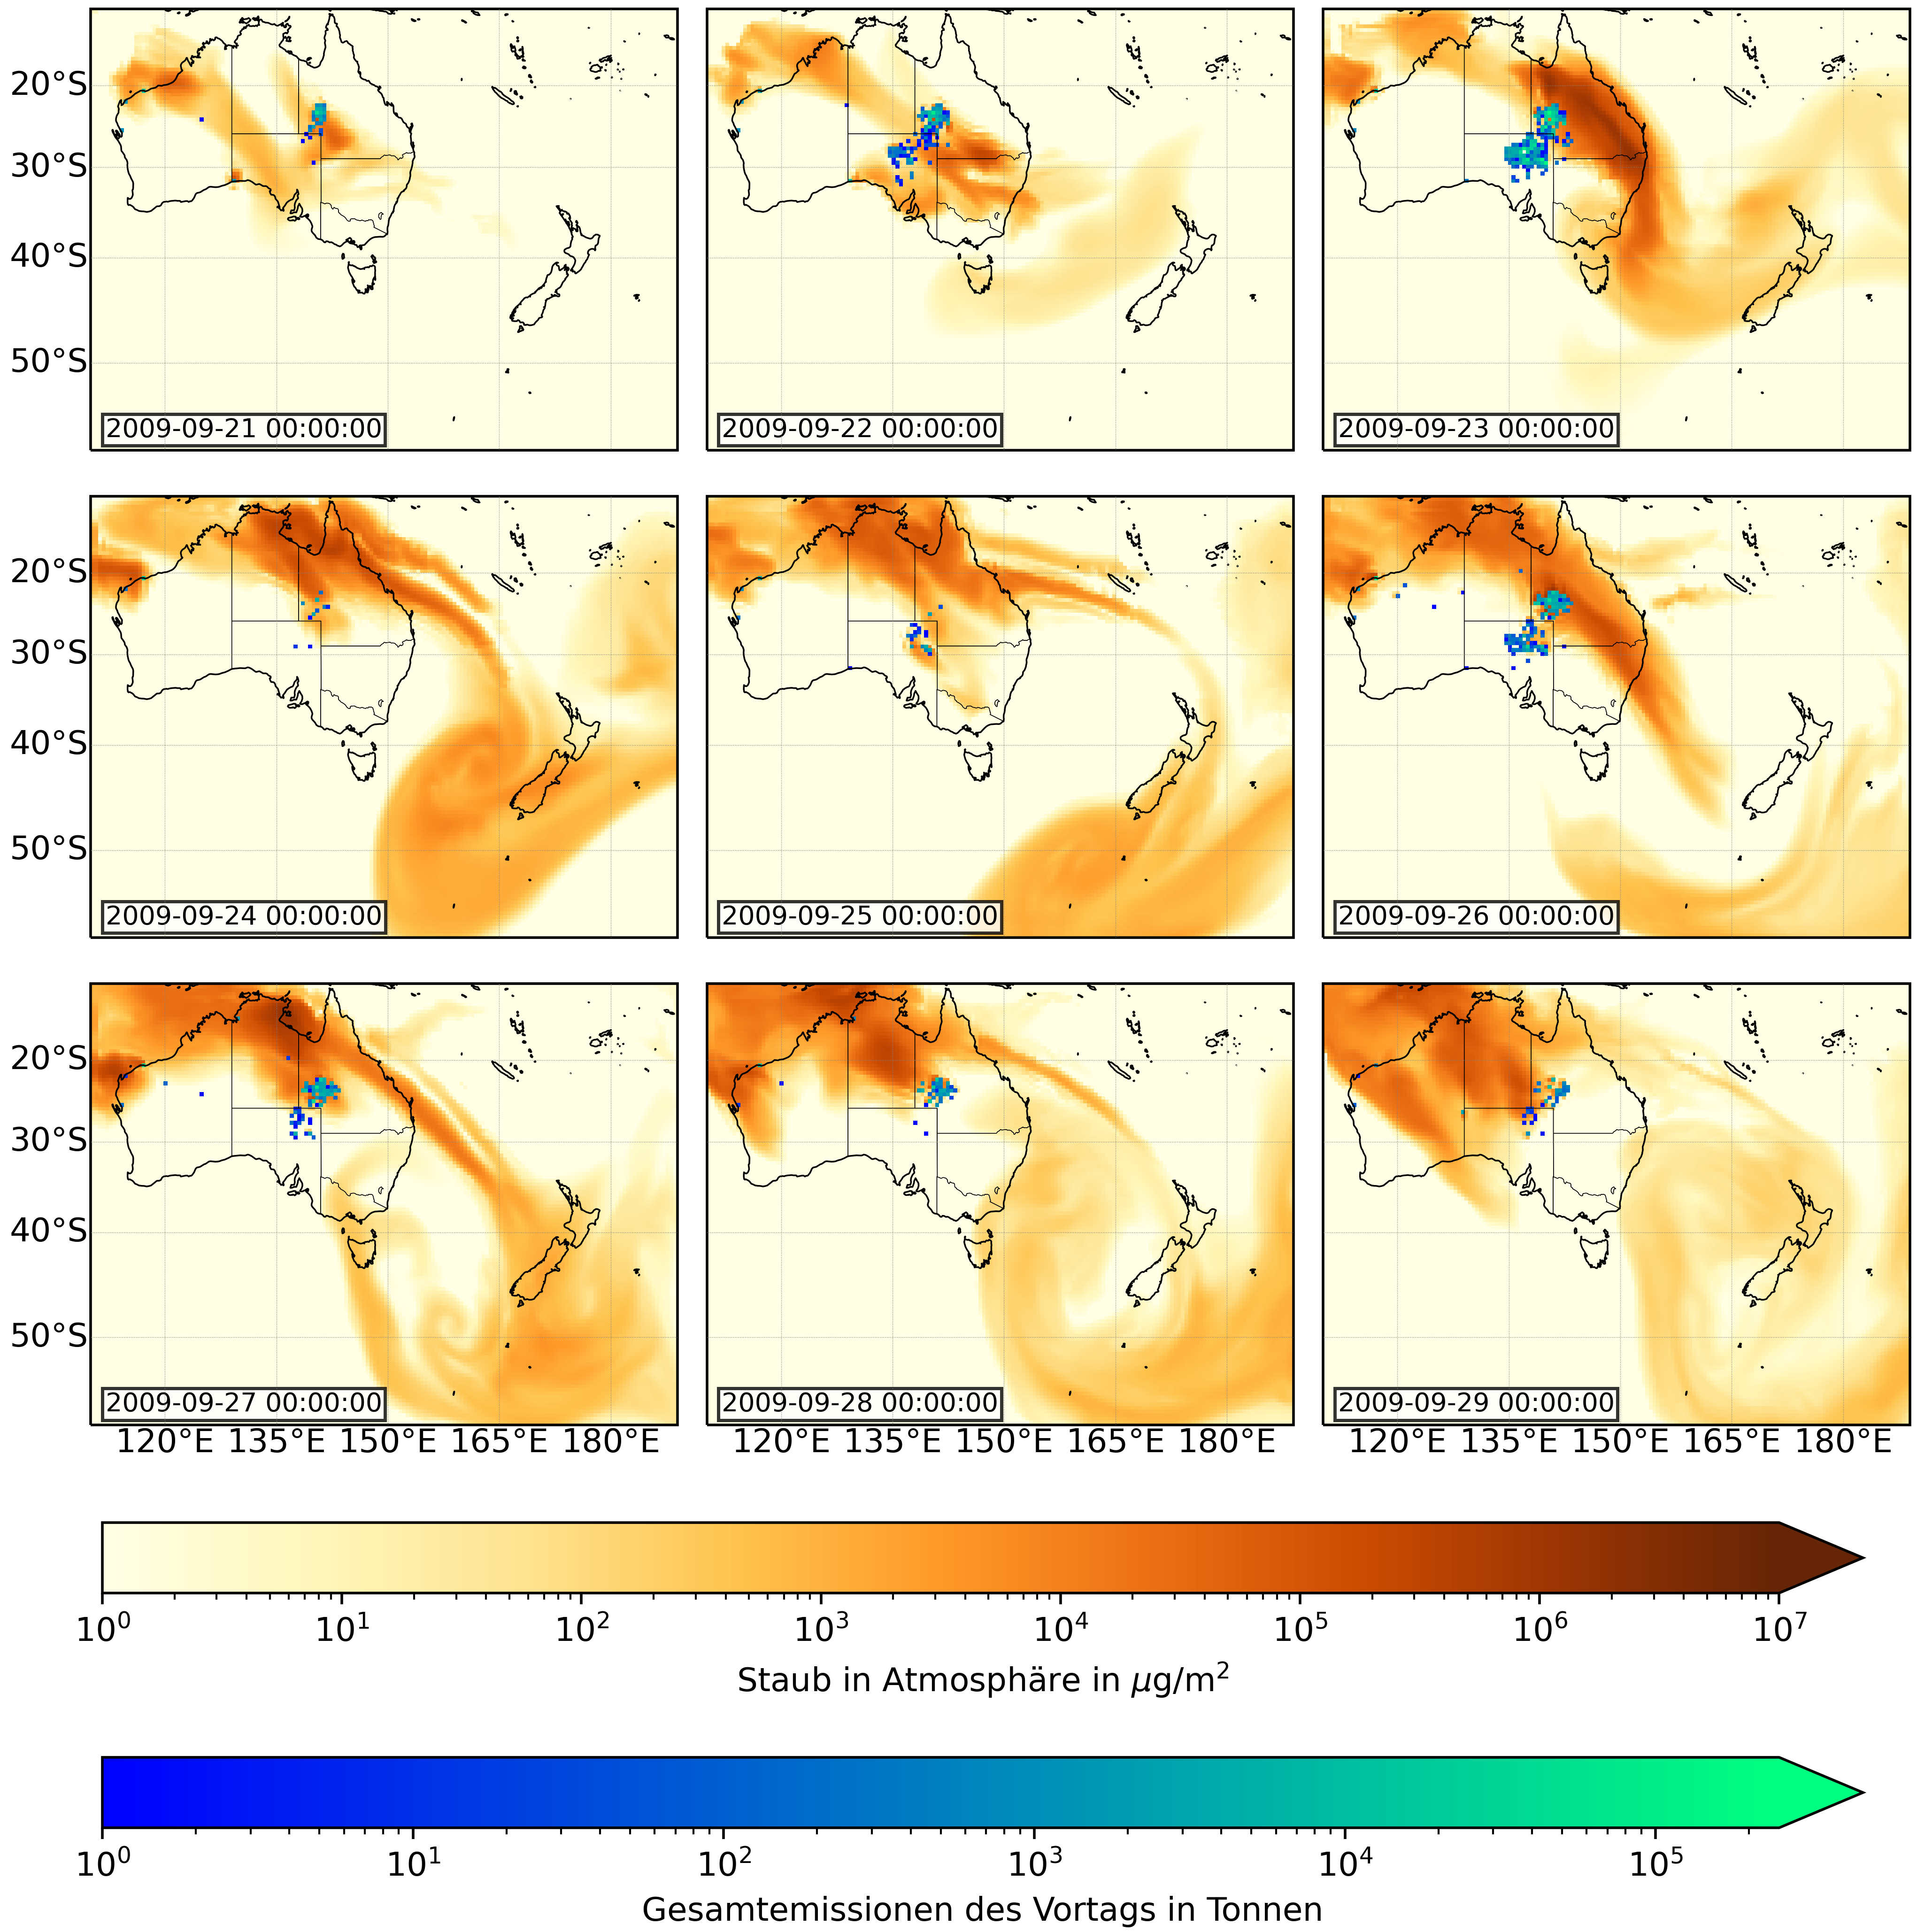
\includegraphics[width=\textwidth]{bilder/dustload.png}
\caption{Anschauliche Darstellung der durch das WRF-Modell simulierten Ausdehnung der Staubwolke und der Emissionsquellen für die 9 relevanten Tage jeweils zu 0 Uhr UTC. Jeweils unten links in der Textbox sind die bis zum genannten Zeitpunkt kumulierten Tages-Emissionen in Tonnen ausgegeben. Der mit Abstand größte Teil (1974 tausend Tonnen bzw. knapp 2Tg) wird demnach am 22. September emittiert. } \label{fig:dustload}
\end{figure}
Die Simulation präsentiert zwei Regionen, welche die wesentlichen Hauptquellen darstellen: 1) \textit{Channel Country} im Westen von Queensland und 2) große Teile des Lake Eyre Beckens in Südaustralien, siehe Abbildung \ref{fig:emissions}. Knapp zwei Drittel stammen aus der Region Channel Country, etwa ein Drittel aus dem etwas südlicheren Teil des Lake Eyre Beckens. Beide Quellen wurden in vorangegangenen Arbeiten ebenfalls identifiziert (sh. Kapitel \ref{sec:reddawn}). Die weiteren mutmaßlichen Quellen (Bergbaugebiete um Cobar und Broken Hill und Weideland im Nordwesten von New South Wales) spielen in der Simulation allerdings keine Rolle. Darüber hinaus wird der Großteil des Staubes von nur einigen wenigen Gitterzellen emittiert. Die Gesamtemission beträgt 3.4 Millionen Tonnen (= 3.4 Tg, davon 2.3 Tg bis zum 23.09. um 0 Uhr UTC). Davon werden allein 650 tausend Tonnen, also etwa 19 \% von nur einer Zelle in Channel Country abgetragen, welche eine Landfläche der Größe von etwa 2462 Quadratkilometer repräsentiert. Im Modell wird die Landfläche Australiens durch 3226 Gitterpunkte abgebildet. Davon emittieren 195 Staub, wovon wiederum nur 6 fast die Hälfte (48.9 \%) der Gesamtemissionen ausmachen. 75 \% werden bereits von 20 Quellen repräsentiert, 42 sind für über 90 \% verantwortlich, sh. Abbildung \ref{fig:emissions}. 
\begin{figure}
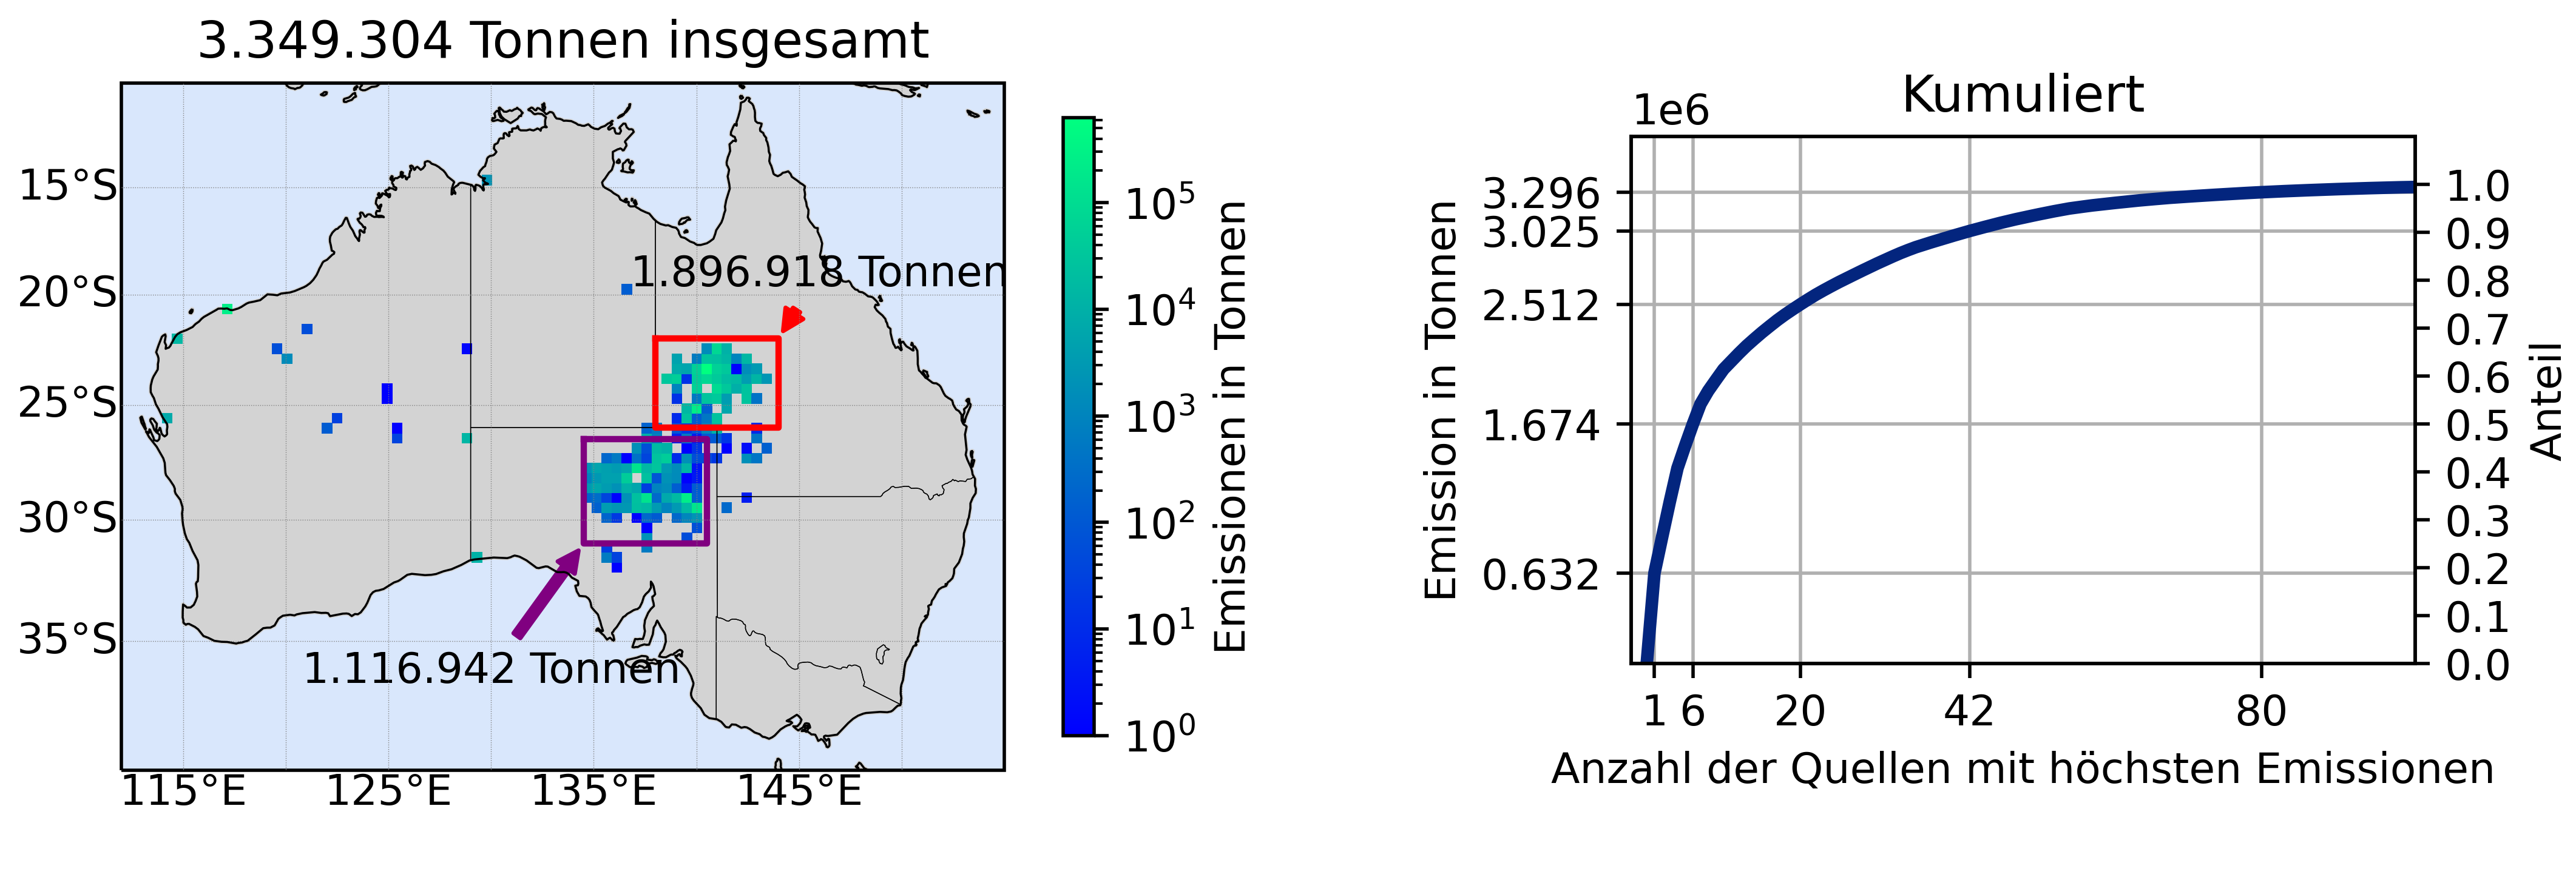
\includegraphics[width=\textwidth]{bilder/emission_sections.png}
\caption{Links: Darstellung der Staubquellen bei Angabe der Gesamtemissionen je Gitterpunkt. Es werden grob zwei Hauptregionen identifiziert: Channel Country (roter Kasten) und das Lake Eyre Becken in Südaustralien (violetter Kasten). Rechts: Darstellung der Abhängigkeit von einzelnen Quellen. Die logarithmisch ansteigende Kurve zeigt, dass wenige Gitterpunkte einen Großteil der Emissionen beschreiben.} \label{fig:emissions}
\end{figure}
Die Staubwolke erreicht ca. am 22. September um 9 Uhr UTC mit knapp 1.2 Tg ihre maximale Beladung, siehe Abbildung \ref{fig:dustload_time}. Über die Hälfte des Staubs wird noch am 23. September wieder auf Land- und Ozeanflächen eingetragen. Durch zusätzliche Emissionen am 28. September halten die maximalen Staubkonzentrationen beim zweiten Hauptereignis ab dem 26.09. etwas länger an, die absoluten Werte liegen aber etwa bei der Hälfte des größeren Ereignisses vom 23. September. Zum Ende der Simulation befinden sich noch etwa 0.2 Tg Staub in der Atmosphäre (d.h., ohne Berücksichtigung des Teils außerhalb des Untersuchungsgebietes).
\begin{figure}
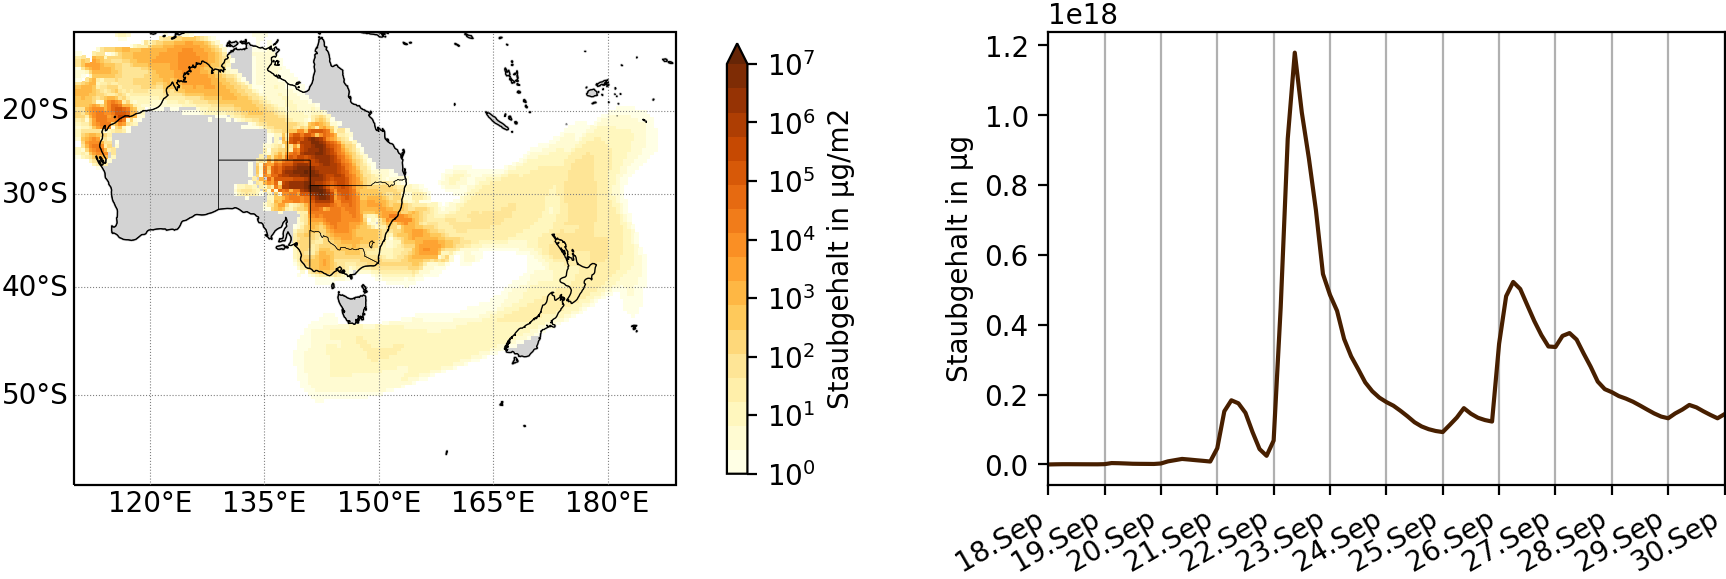
\includegraphics[width=\textwidth]{bilder/dustload_time.png}
\caption{Links: Maximale Ausdehnung der Staubwolke am 22. September um 9 Uhr UTC. Rechts: Zeitserie des Staubgehaltes in der Atmosphäre für den kompletten Simulationszeitraum} \label{fig:dustload_time}
\end{figure}
Von den etwa 3.4 Tg Staubemissionen werden innerhalb des WRF-Simulationszeitraums etwa 1.7 Tg wieder auf Land- und Ozeanflächen eingetragen. Abbildung \ref{fig:deposition} zeigt, dass der Großteil des Staubs laut Modell in direkter Nähe zur Quelle trocken wieder eingetragen wird. Nur ein geringer Teil erreicht tatsächlich den Ozean der hier betrachteten Domäne, ein großer Teil wird nördlich und westlich außerhalb abtransportiert. 
\begin{figure}
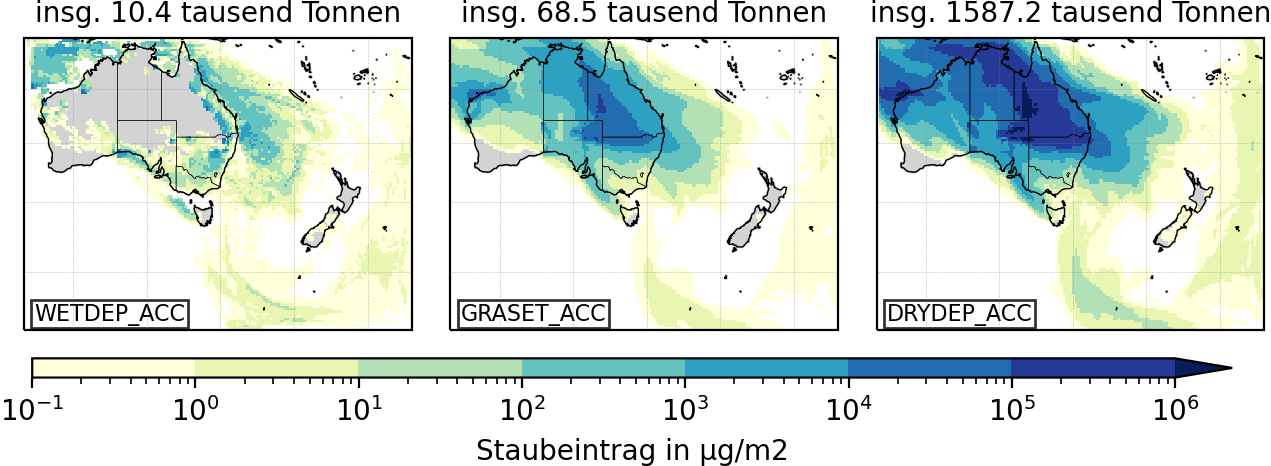
\includegraphics[width=\textwidth]{bilder/dust_deposition_vars.png}
\caption{Kumulierter Eintrag von Staub über den gesamten Simulationszeitraum. Der Gesamteintrag ergibt sich als Summe von nassem Eintrag (links, Auswaschung durch Regen), Ablagerung durch Gravitation (Mitte) und trockenem Staubeintrag (rechts).} \label{fig:deposition}
\end{figure}
Ein ähnliches Muster zeigt sich bei den darin enthalten Eisendepositionen (Abb. \ref{fig:iron_deposition}). Insgesamt werden lt. Simulation knapp 19 tausend Tonnen (0.019 Tg) Eisen eingetragen. Wesentlicher Unterschied ist allerdings, dass hier der Eintrag aufgrund der Erdbeschleunigung (\textit{gravitional settling}) dominiert. In beiden Fällen erreicht nur ein sehr kleiner Bruchteil den für die Eisenhypothese wichtigen südlichen Ozean.
\begin{figure}
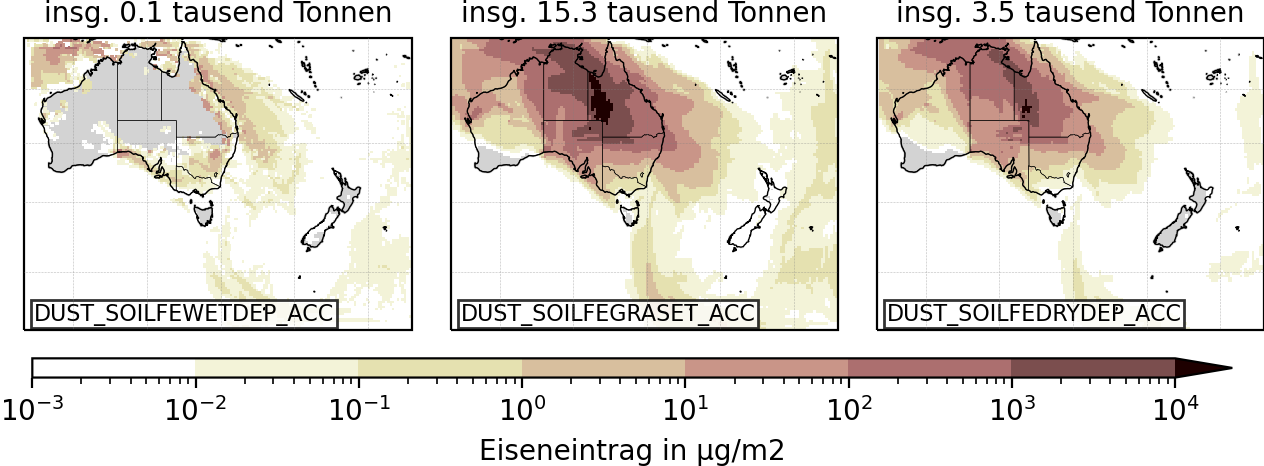
\includegraphics[width=\textwidth]{bilder/iron_deposition_vars.png}
\caption{Kumulierter Eintrag von Eisen über den gesamten Simulationszeitraum. Der Gesamteintrag ergibt sich als Summe von nassem Eintrag (links, Auswaschung durch Regen), Ablagerung durch Gravitation (Mitte) und trockenem Staubeintrag (rechts).} \label{fig:iron_deposition}
\end{figure}
Im folgenden wird der Eiseneintrag etwas genauer analysiert. Hierzu wird die Domäne in 5 Regionen unterteilt. In Abbildung \ref{fig:iron_deposition_sections} ist das räumliche Muster der Eisendepositionen mit den zugehörigen Zeitserien dargestellt. Zeitpunkt und Höhe des Eintrag unterscheiden sich je nach Region deutlich. Insgesamt werden etwas über 2.000 Tonnen, also knapp 11 \% der Gesamtdepositionen in den Ozean eingetragen, davon der überwiegende Teil mit knapp 1.900 Tonnen im Nordosten am 26. und 27. September. Weniger als ein Zehntel davon wird lt. WRF-Modell in das Korallenmeer und das Tasmanische Meer eingetragen. Diese Depositionen ereignen sich wenige Stunden nach dem Red Dawn am 23. September. In den Süden und den Südozean wird vergleichsweise wenig eingetragen. Wie in der Zeitreihe auf Abb. \ref{fig:iron_deposition_sections} zu sehen, wird ein Teil des Staubs scheinbar erst nach dem Simulationszeitraum eingetragen, da weiterhin Staub in der Atmosphäre ist (vgl. Abb. \ref{fig:dustload_time}).
\begin{figure}
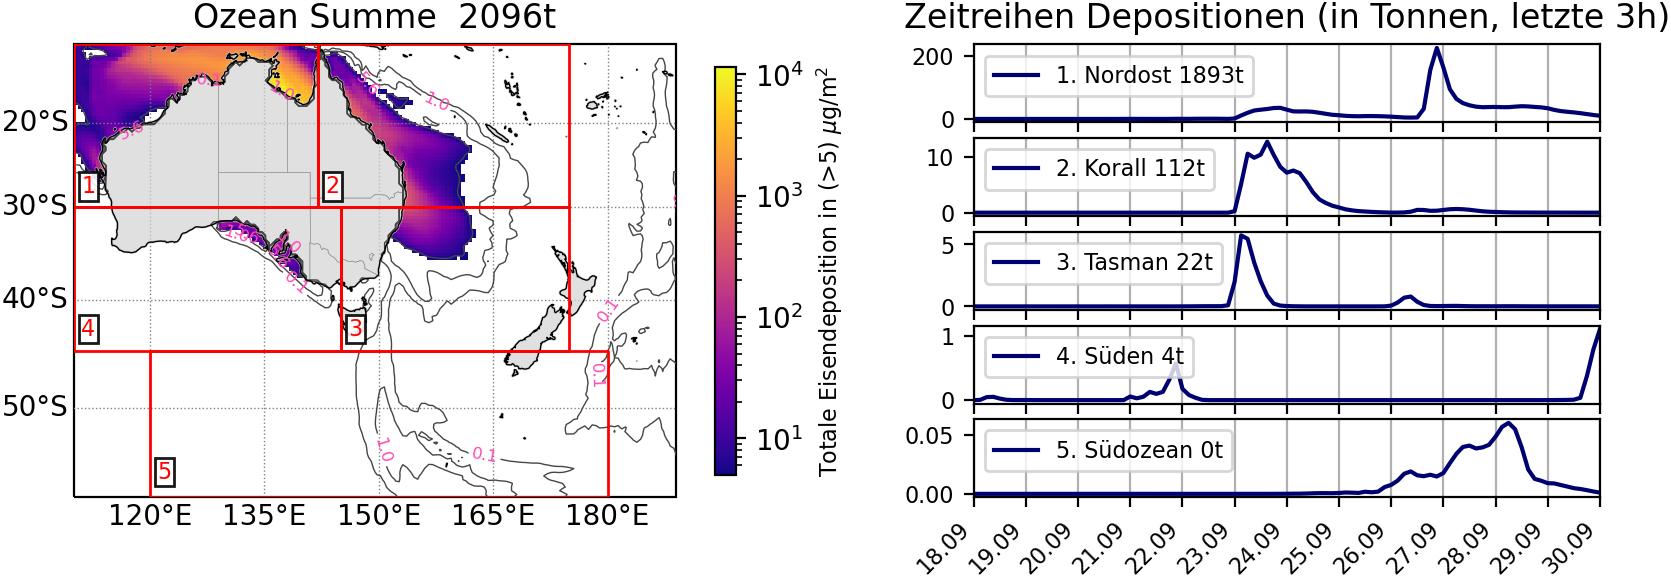
\includegraphics[width=\textwidth]{bilder/total_iron.png}
\caption{Vom WRF-Modell simulierter Eiseneintrag. Die Domäne wird in 5 Sektoren unterteilt: 1. Nordosten, 2. Korallenmeer, 3. Tasmanisches Meer, 4. Süden, 5. Südozean. Die farbige Kontur gibt die Höhe der des Eintrags für alle Regionen mit einem Eintrag größer als 5.6 µg/m2 an. Kleinere Einträge sind durch die grauen Konturlinien (1 und 0.1 µg/m2) angezeigt. Rechts sind die jeweiligen Zeitserien der Eisendepositionen für die Regionen dargestellt.} \label{fig:iron_deposition_sections}
\end{figure}
\subsection{Chlorophyll-a Zeitreihen} \label{sec:chla_zeitreihen}
Abbildung \ref{fig:chla_collage} zeigt anschaulich, dass die Chlorophyll-a-Konzentrationen zwischen Australien und Neuseeland (im Tasmanischen Meer) nach dem Staubsturm (d.h. dem Hauptereignis am 23.09.) ansteigen. Maximale Werte treten demnach am 1. und 2. Oktober auf. Das mutmaßlich aufgrund der Wirbel der tasmanischen Front \citep{Gabric.2016} entstandene Muster ist heterogen, Regionen mit hohen Cholorophyll-a-Konzentrationen sind auf entsprechend geformte Bereiche in der turbulent anmutenden Struktur beschränkt. Unabhängig von der Entwicklung ist sichtbar, dass die Konzentrationen nördlich von 25-30°S (etwas nördlich der Grenze New South Wales und Queensland) auch im Vergleich zum Südozean per se deutlich geringer sind. Da die Küsten selbst Eisenquellen sein können und/oder je nach Strömungsverhätlnissen Regionen mit aufsteigendem nährstoffreichen Wasser bieten können, sind die Konzentrationen dort i.d.R. höher als auf dem offenen Ozean. Besonders an der Nordostküste Queenslands offenbart sich ein beschränkter Bereich mit deutlich höheren Chlorophyll-Konzentrationen als in der Umgebung. 
\begin{figure}
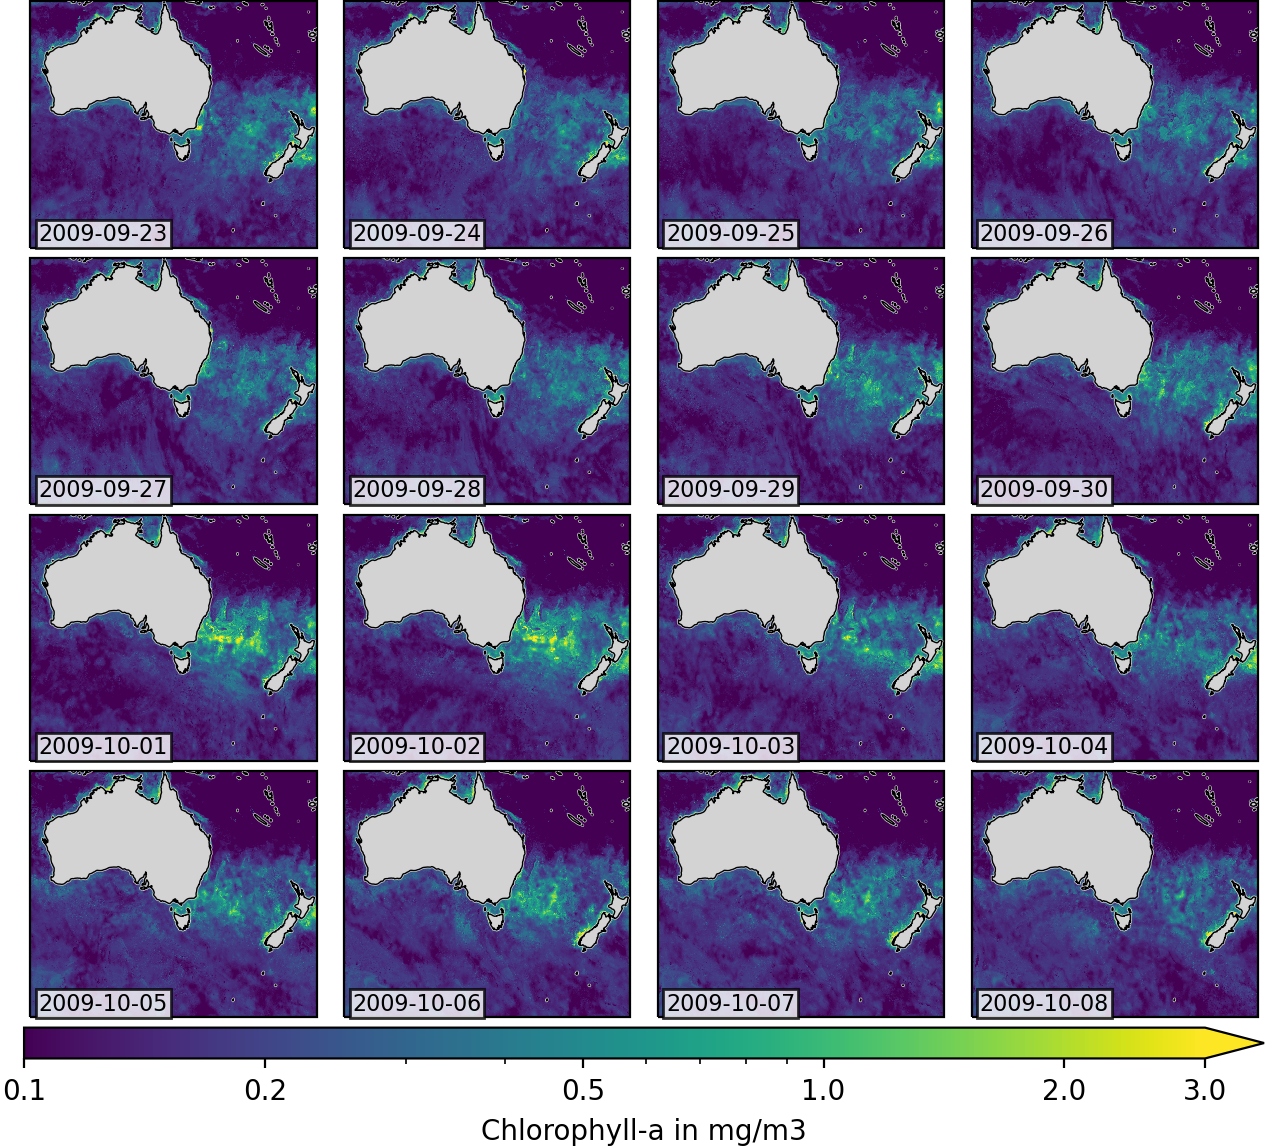
\includegraphics[width=\textwidth]{bilder/chl_collage.png}
\caption{Die Rohdaten für die weitere Analyse: Chlorophyll-a-Konzentrationen für den Zeitraum ab kurz nach dem \textit{Red Dawn Event} bis mehrere Tage danach. Die täglichen Beobachtungsdaten wurden gemäß \cite{Saulquin.2019} interpoliert und über den Marine Copernicus Service zur Verfügung gestellt (2009XXXX_d-ACRI-L4-CHL-MULTI_4KM-GLO-REP).} \label{fig:chla_collage}
\end{figure}
Um die Entwicklung des Phytoplanktons genauer zu untersuchen, werden im folgenden Zeitreihen der Chlorophyll-a-Konzentrationen untersucht. Entsprechend Kapitel \ref{sec:timeseries} werden die Mittelwerte für die in Abbildung \ref{fig:iron_deposition_sections} gezeigten 5 verschiedenen Regionen gebildet und deren Zeitreihen für den Zeitraum Juni bis Dezember 2009 präsentiert. Hierbei wurden die Gitterpunkte ausgeschlossen, die direkt an Landfläche grenzen und damit die Küstenzone (etwa 50km Ausdehnung) repräsentieren. Diese Zonen weisen im Datensatz außerordentlich hohe Werte und Variabilitäten auf, welche mutmaßlich aufgrund von Flussmündungen oder besonderen Wechselwirkungen mit der Küste auftreten. Diese besonderen Effekte können bei der Mittelwertbildung zu Verzerrungen führen. In der rechten Spalte von Abb. \ref{fig:timeseries_full} wird dieselbe Zeitreihe um den jahreszeitlichen Trend bereinigt (, gefiltert) und gleichzeitig die Region auf die Gitterpunkte beschränkt, für die das WRF-Modell einen Gesamtstaubeintrag von mehr als 5 µg pro Quadratmeter simuliert. Diese Änderungen in der Darstellung helfen, ein möglicherweise mit den Staubdepositionen verbundenes Signal zu identifizieren. Ist das Signal der räumlich weiter eingeschränkten Region (in der rechten Spalte) deutlicher als jenes für die gesamte Region (linke Spalte), ist dies sowohl für eine erfolgreiche Simulation der Staub- bzw. Eisendepositionen als auch einen etwaigen Zusammenhang ein positives Indiz. 
\begin{figure}
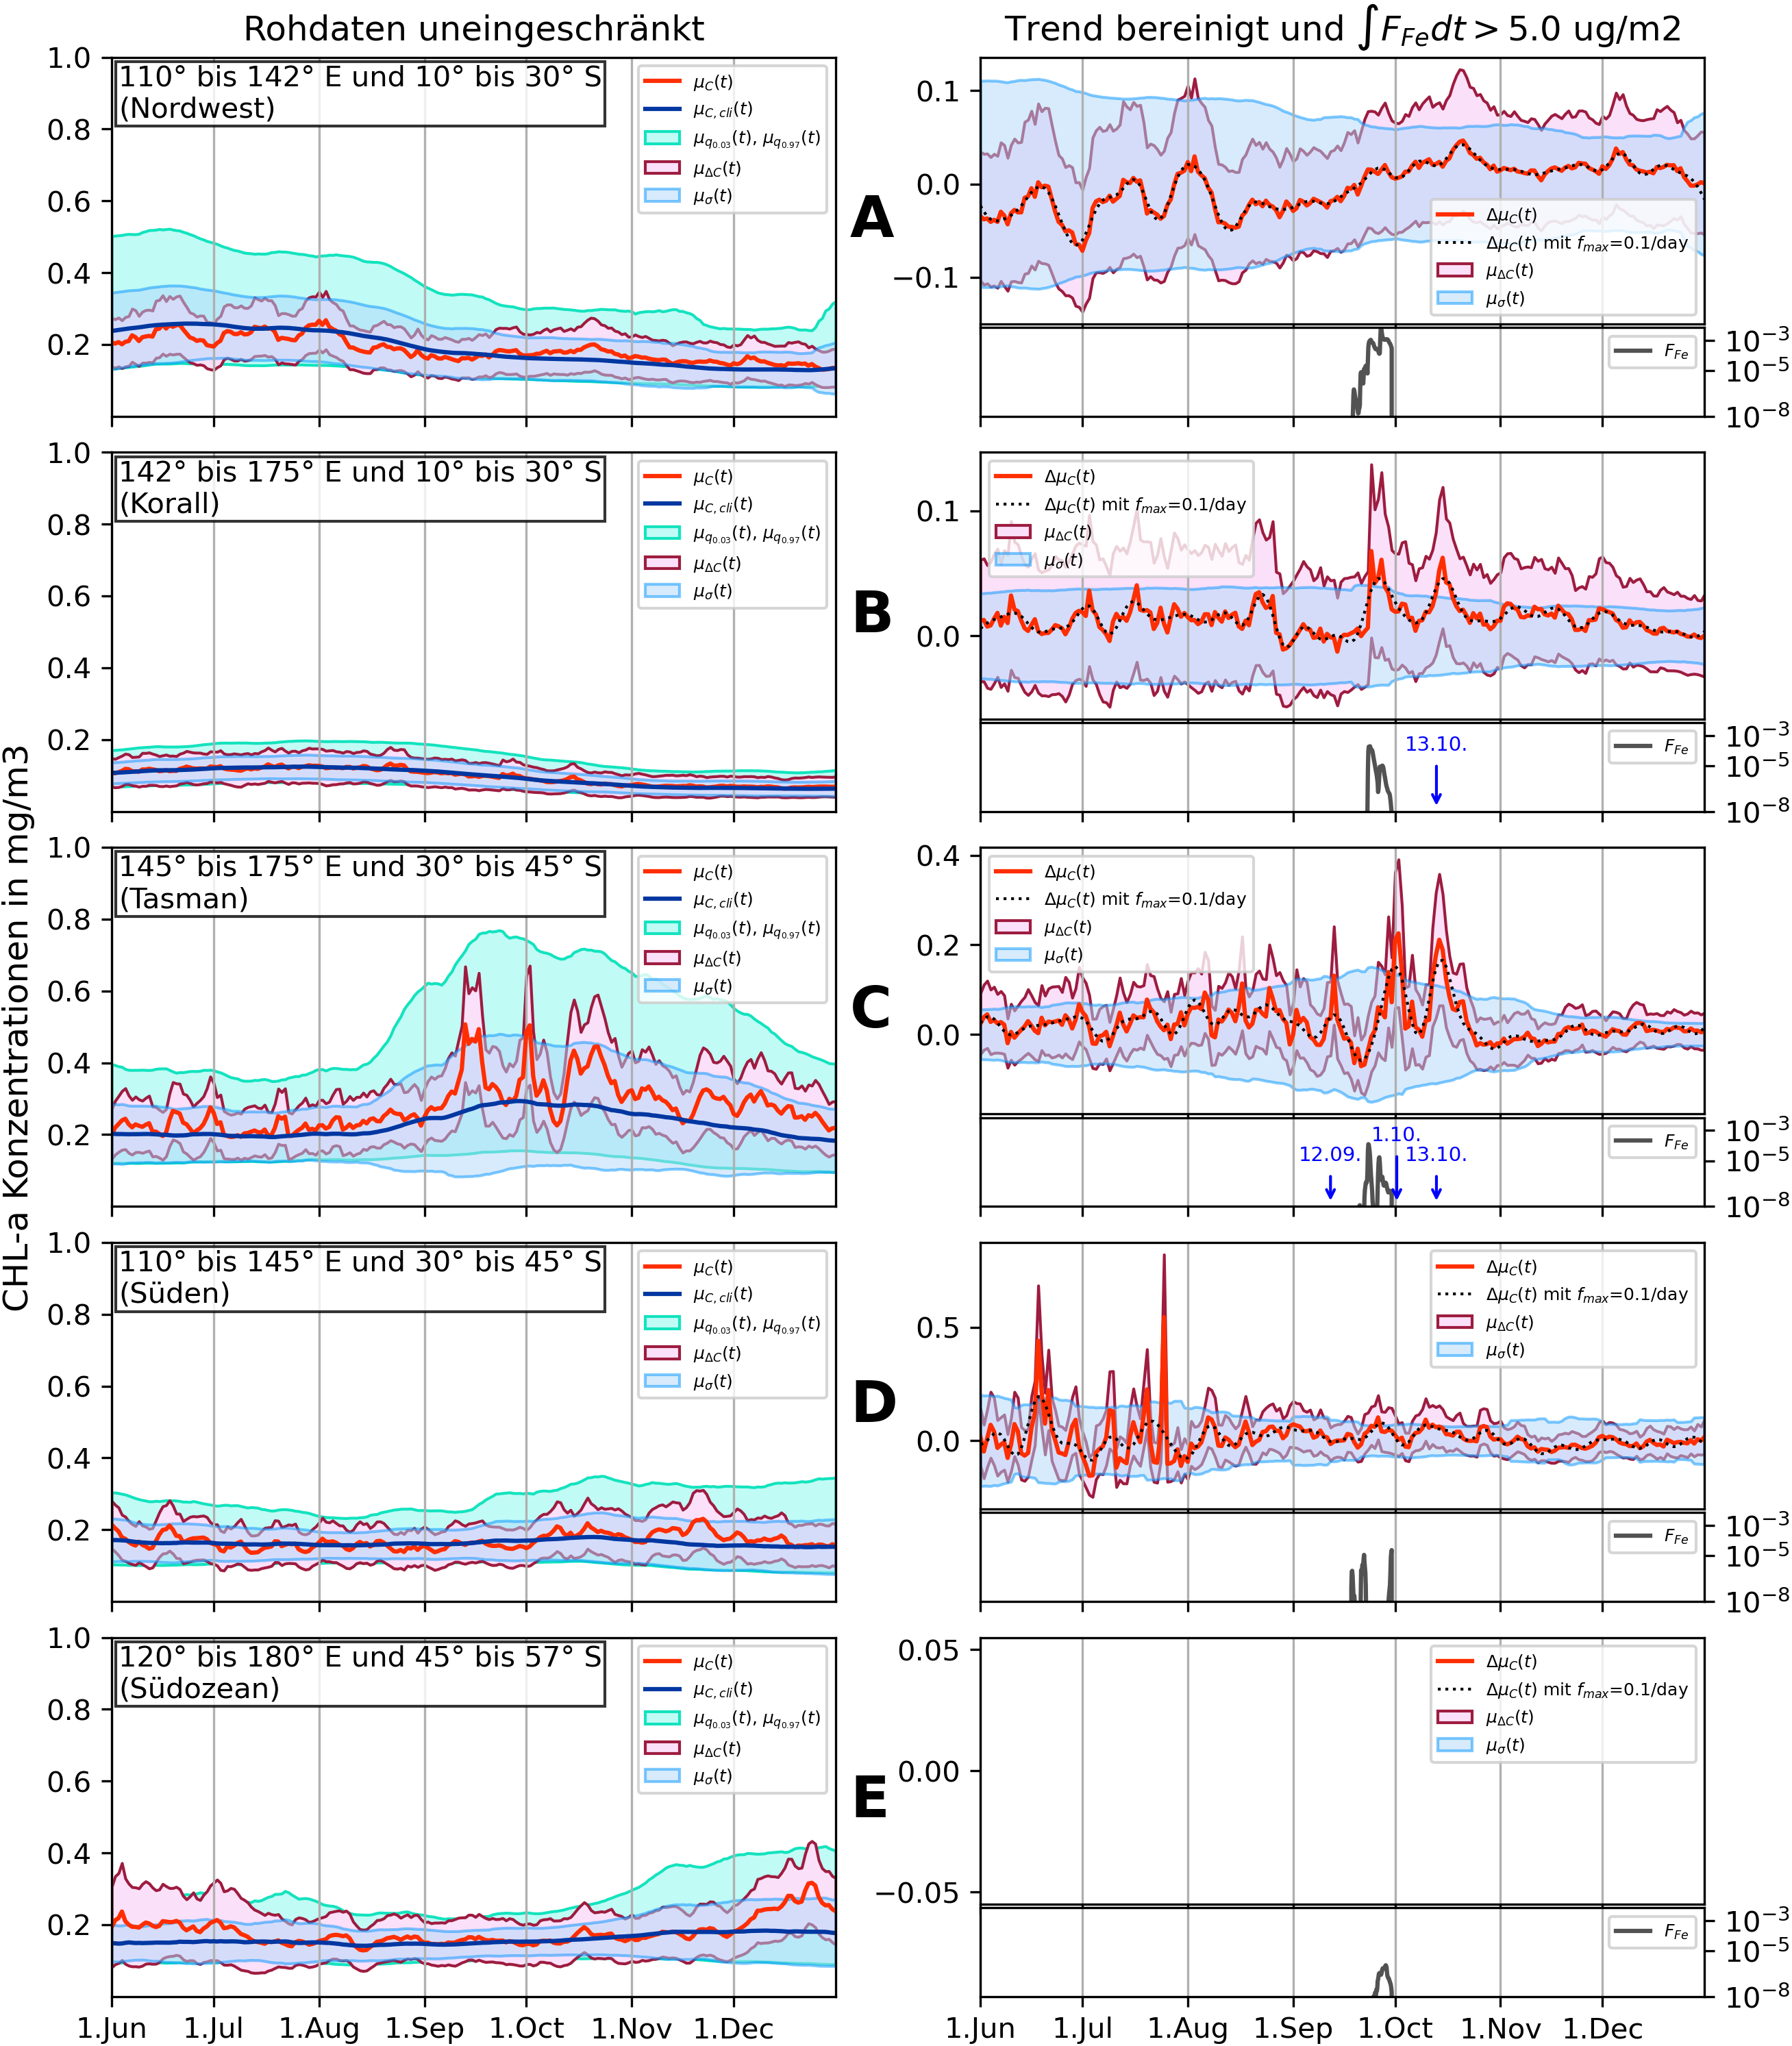
\includegraphics[width=\textwidth]{bilder/timeseries_all.png}
\caption{Zeitreihen vom 1. Juni bis 31. Dezember 2009 der mittleren Chlorophyll-a Konzentrationen für die gemäß Abb. \ref{fig:iron_deposition_sections} unterteilten Gebiete in den jeweiligen Zeilen \textbf{A} bis \textbf{E}. Links ist jeweils die Zeitreihe der Mittelwerte für die komplette Region (ohne Einschränkungen) abgebildet. Rechts daneben in der zweiten Spalte wurden diese \textit{Rohdaten} um die Klima-Mittelwerte korrigiert und das Untersuchungsgebiet auf diejenigen Gitterpunkte beschränkt, für eine Eisendeposition $m_\text{Fe}$ von mehr als 5µg pro qm simuliert wurde. Zusätzlich wurde das Signal mithilfe eines Tiefpassfilters geglättet. Rechts unten sind die Zeitreihen der Eisendepositionen für die jeweilige Region dargestellt. Die Pfeile markieren möglichen weiteren Staubeintrag auf Basis der Satellitenbilder in Abb. \ref{fig:duststorms_surrounding}. Für die Beschreibung der Variablen siehe Kapitel \ref{sec:timeseries}}. \label{fig:timeseries_full}
\end{figure}
Anhand Abb. \ref{fig:timeseries_full} ist zu erkennen, dass sich die mittleren Chlorophyll-a-Konzentrationen je nach Region stark unterschieden. So sind bspw. Variabilität und Absolutwerte im Korallenmeer (Abb. \ref{fig:timeseries_full} B) im Vergleich zum sehr viel dynamischeren Tasmanischen Meer (Abb. \ref{fig:timeseries_full} C) sehr gering. Anhand der jeweils auf denselben Wertebereich (0 bis 1 mg/m3) eingeschränkten Beobachtungsdaten in der ersten Spalte sind außer für das Tasmanische Meer kaum nennenswerte Abweichungen von den Klimawerten zu erkennen. Im Tasmanischen Meer (Abb. \ref{fig:timeseries_full} C) sind drei relativ deutliche Signale (positive Abweichungen von den Klimadaten) Mitte September, am 1. Oktober und erneut Mitte Oktober identifizierbar. Allerdings sind genau zu dieser Zeit auch Standardabweichung und das 97 \% Perzentil der Klimadaten deutlich höher als im restlichen Zeitraum, die Maximalwerte liegen immer noch deutlich unter dem 97 \% Perzentil. Das lässt darauf schließen, dass zwischenzeitlich erhöhte Chlorophyll-a-Konzentrationen in dieser Region regelmäßig auftreten und möglicherweise mit anderen Prozessen wie den mit dem Ostaustralstrom assoziierten Wirbeln und einem jahreszeitlichen Gang \citep{Tilburg.2002} verbunden sind. Die Signale aus Mitte September und Mitte Oktober liegen beide außerhalb des Simulationszeitraums und es wird nicht angenommen, dass das hier vordergründig untersuchte Staubereignis vom 23. September 2009 noch einen maßgeblichen Einfluss auf die erhöhten Werte Mitte Oktober gehabt haben kann. Allerdings kann für beide Signale ebenfalls ein Zusammenhang mit Staubdepositionen vermutet werden, da zu beiden Zeiten vermehrte Staubaktivität beobachtet wurde (siehe Abbildung \ref{fig:duststorms_surrounding}). 
\begin{figure}
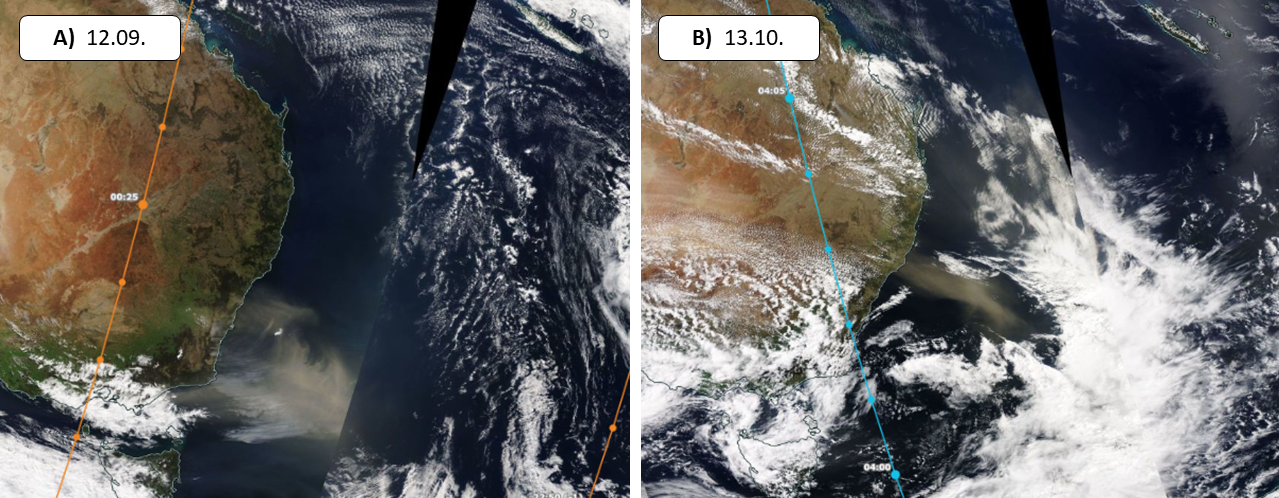
\includegraphics[width=\textwidth]{bilder/duststorms_surround.png}
\caption{Satellitenfotos, aufgenommen mit NASA Worldview. A) Aufnahme TERRA vom 12. September zeigt Staub über dem Tasmanischen Meer. B) Aufnahme AQUA vom 13. Oktober 2009 zeigt ebenfalls Staub über dem Tasmanischen Meer, allerdings etwas nördlicher als in A). } \label{fig:duststorms_surrounding}
\end{figure}
In der rechten Spalte von Abb. \ref{fig:timeseries_full} C ist der jahreszeitliche Trend eliminiert worden. Das Signal aus Mitte September ist hierauf deutlich schwächer ausgeprägt. Dies korrespondiert mit der Beobachtung, dass das möglicherweise zugehörige Staubereignis (siehe Abbildung \ref{fig:duststorms_surrounding} A) weiter südlich aufgetreten ist als der Staubeintrag gemäß unserer WRF-Simulation. Die erhöhten Werte Mitte Oktober treten hingegen auch in der bereinigten Zeitreihe auf, was aber auch zur räumlichen Ausdehnung entsprechend dem Satellitenbild (Abb. \ref{fig:duststorms_surrounding} B) passt. Von zentraler Bedeutung für diese Analyse ist jedoch mutmaßlich das deutliche Signal in Abb. \ref{fig:timeseries_full} C (rechts) gegen Ende September/Anfang Oktober, welches demnach etwa 5-6 Tage nach dem simulierten Haupt-Eisentrag vom 23. September eintritt. Dieses ist insgesamt am höchsten und übertrifft immerhin knapp die mittlere Standardabweichung $\mu_\sigma(t)$ der Klimadaten. Obwohl die Variabilität in dieser Region augenscheinlich ohnehin sehr groß ist, wird angenommen, dass diese erhöhten Chlorophyll-a-Konzentrationen auf das \textit{Red Dawn Event} zurückzuführen sind. Bei \citet{Martin.1988} tritt eine Reaktion des Phytoplanktons nach etwa 4 Tagen auf. Unter realistischen Bedingungen ist eine etwas spätere Reaktion plausibel, da die innerhalb des Staubs auftretenden Eisenpartikel weniger gut löslich sein können \citep{Shao.2011}. Dass dieser zeitliche Zusammenhang zufällig auftritt, erscheint auch angesichts der \textit{benachbarten} Ereignisse Mitte September und Mitte Oktober unwahrscheinlich. \\

Neben dem Tasmanischen Meer sind auf Abbildung \ref{fig:timeseries_full} auch für das Korallenmeer (\textbf{B}, rechts) erhöhte Durchschnittswerte für Ende September/Anfang Oktober und Mitte Oktober auffällig. Die absolute durchschnittliche Anomalie $\Delta \mu_C(t)$ liegt mit knapp +0.1 mg/m3 bei weniger als der Hälfte der durchschnittlichen Anomalie des tasmanischen Meers mit über 0.2 mg/m3 zur ähnlichen Zeit. Außerdem wird das Maximum etwas früher erreicht. Anhand der Satellitenbilder (Abb. \ref{fig:satellite}) wird deutlich, das die Staubwolke jedenfalls nahe der Küste einen Großteil des Korallenmeers abgedeckt hat, was unabhängig von der Simulation auf möglichen Staubeintrag hinweist. Auch in den Zeitreihen zu den Regionen im Nordosten und Süden (\ref{fig:timeseries_full} A und D) sind Tendenzen erkennbar, dass die Phytoplankton-Konzentrationen im Oktober nach den Staubdepositionen erhöht waren. Allerdings scheinen hier die Entwicklungen einer tieferen Frequenz zu folgen, es sind keine erheblichen Abweichungen für einzelne Tage erkennbar. Darüber hinaus liegen die Werte stets deutlich innerhalb der Standardabweichung. Für den südlichen Ozean (bzw. südlich des 45°ten Breitengrad) war der Eiseneintrag lt. WRF-Simulation kleiner als 5 µg, weshalb die Zeitreihe in Abbildung \ref{fig:timeseries_full} E leer bleibt. In der (zugegebenermaßen hierfür ungeeignet skalierten) Zeitreihe in der ersten Spalte sind keine nennenswerte Signale ableitbar.
\subsection{Räumliche Muster} \label{sec:auswertung_räuml_Muster}
Im vorangegangenen Kapitel \ref{sec:chla_zeitreihen} wird anschaulich gezeigt, dass das Phytoplankton (d.h. die Chlorophyll-a-Konzentrationen) mindestens in den Regionen um das Tasmanische Meer und dem Korallenmeer mit bzw. kurz nach dem Staubeintrag reagiert. In diesem Kapitel soll der zeitliche Zusammenhang genauer untersucht werden. Unter der Annahme, dass ausschließlich (der korrekt simulierte) Eiseneintrag zu erhöhtem Phytoplankton-Wachstum führt, sollten die Zeitreihen der Depositionen und Chlorophyll-a-Konzentrationen jedes Gitterpunktes stark miteinander korrelieren. Die besondere Fragestellung ist, um welche \textit{Reaktionszeit} $\tau$ die Zeitreihen der Veränderungen der Chlorophyll-a-Konzentrationen gegenüber denen des Eisenflusses verschoben werden müssen, um eine maximale Ähnlichkeit in der Entwicklung zu erreichen. Diese Reaktionszeit könnte dann als die Zeitspanne interpretiert werden, die das Phytoplankton zur Entwicklung benötigt.
\begin{figure}
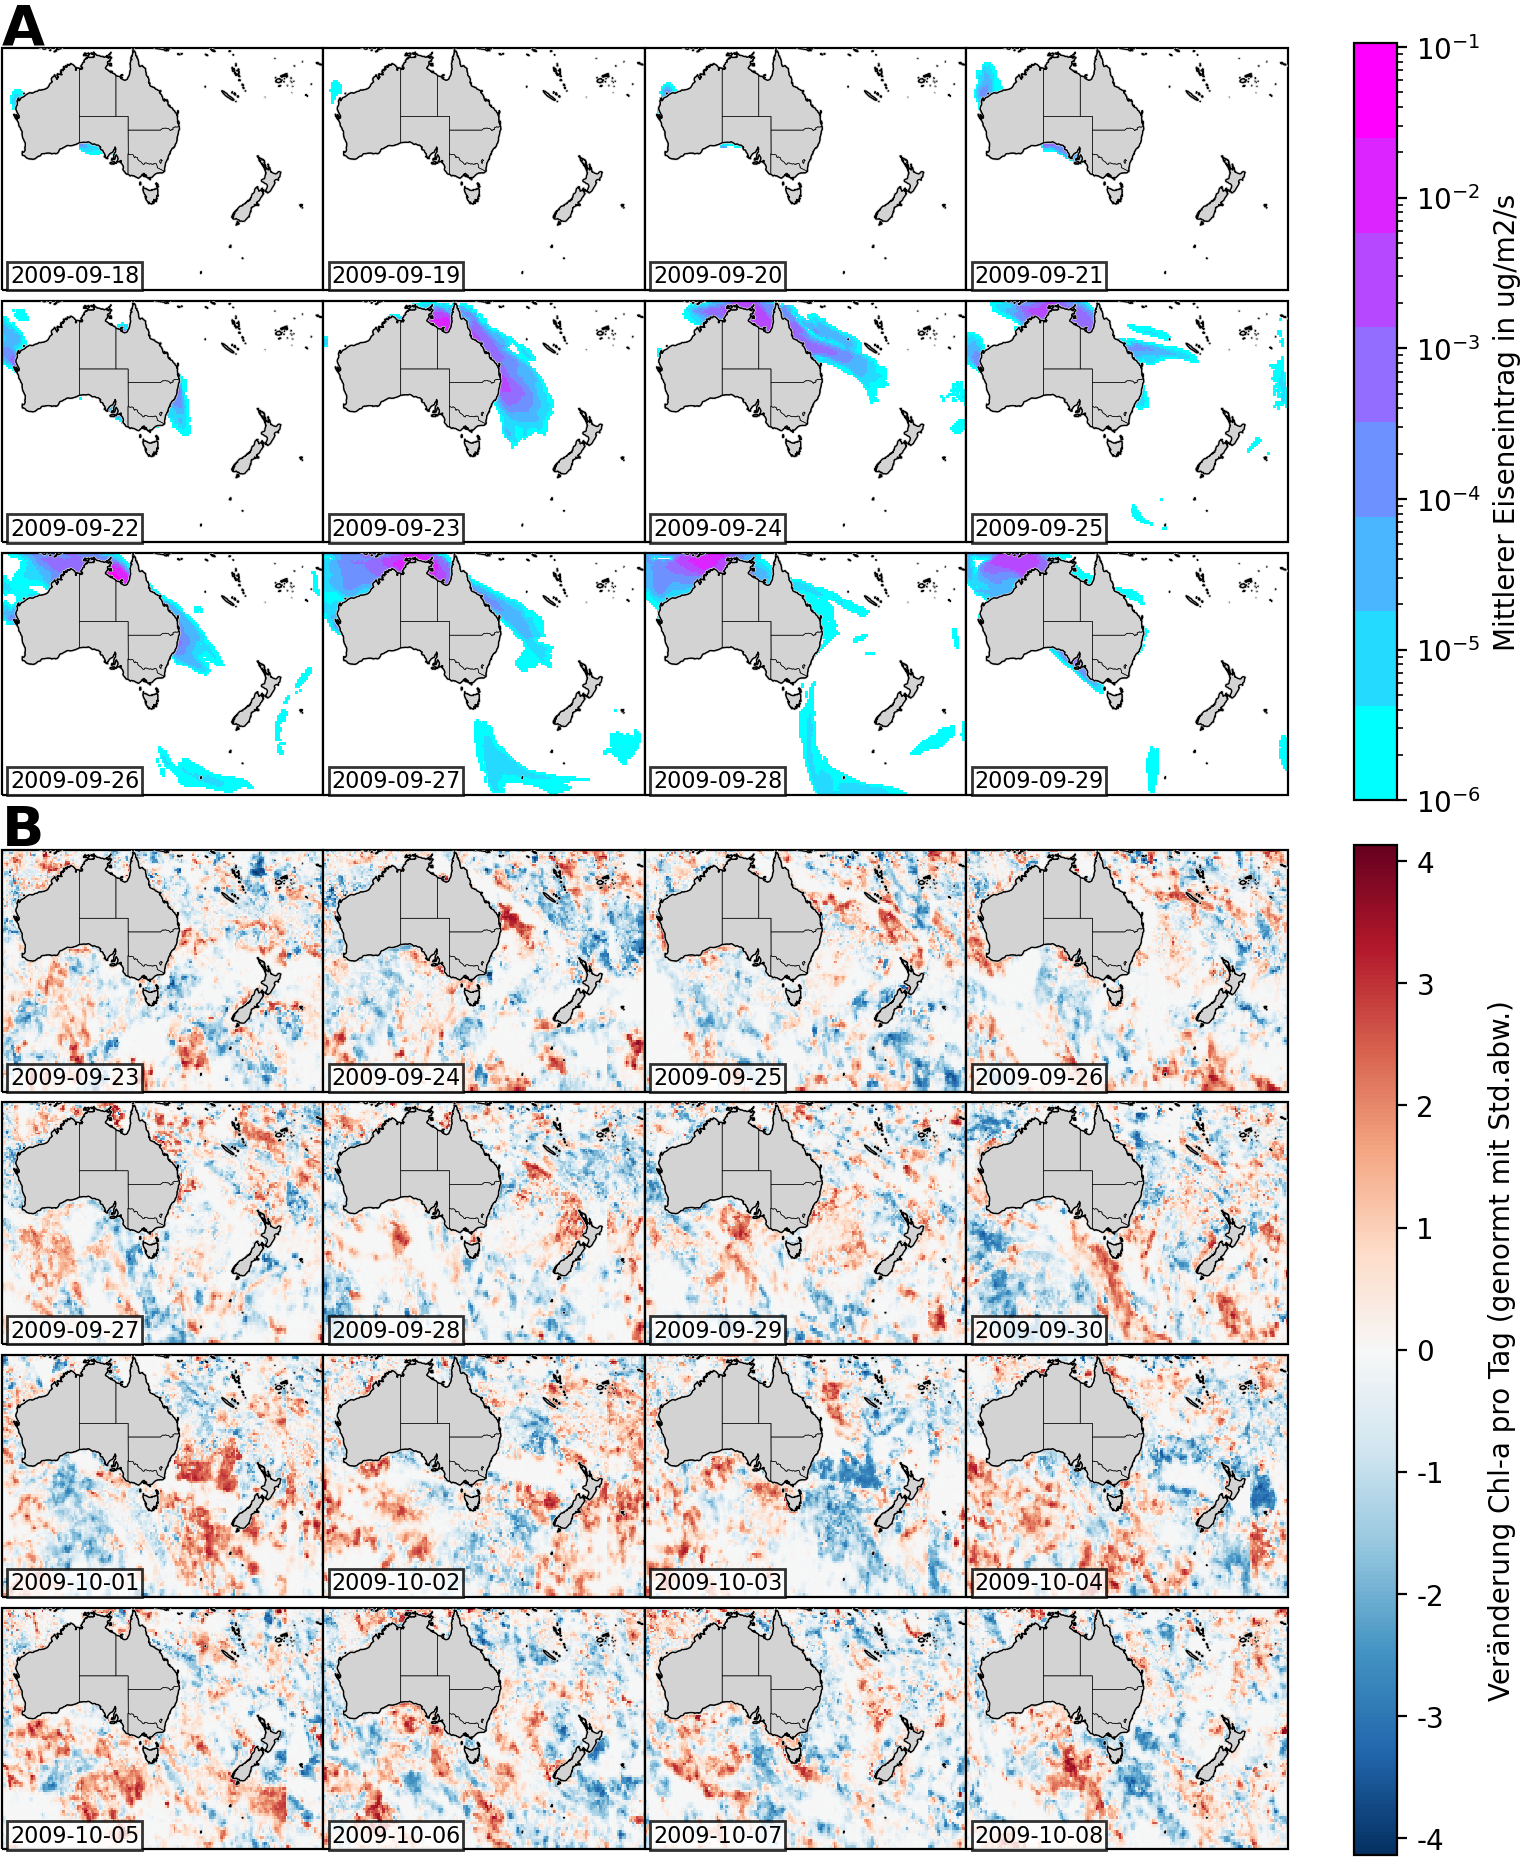
\includegraphics[width=\textwidth]{bilder/snapshot_normalized.png}
\caption{A) Mittlerer Eiseneintrag für die 12 Tage des Simulationszeitraums. B) Tägliche Änderungen der Chlorophyll-a-Konzentrationen ab dem 23. September. Die Werte wurden für jeden Gitterpunkt mit der eigenen Standardabweichung normiert um auch die Muster in Regionen mit geringen Konzentrationen/Abweichungen darzustellen.} \label{fig:snapshot_fedep_chla}
\end{figure}
Wie man Abbildung \ref{fig:snapshot_fedep_chla} entnehmen kann, kann das jeweilige räumliche Muster der Eisendeposition (\ref{fig:snapshot_fedep_chla} A) jedoch nicht überall direkt demselben Muster positiver Werte bei den Chlorophyll-a-Veränderungen (\ref{fig:snapshot_fedep_chla} B) zugeordnet werden. Dies ist erwartungsgemäß, da die Entwicklung des Phytoplanktons bekanntermaßen von weiteren Faktoren abhängig ist, die Simulation der Depositionen nicht perfekt sein kann und auch der düngende Effekt des Eiseneintrags in Form von Staubstürmen in einigen Regionen fraglich ist \citep{Boyd.2010}. Einige Muster sind allerdings auffällig, die hier beschrieben werden sollen. Im Korallenmeer folgt ein Muster positiver Veränderungen der Chlorophyll-a-Konzentrationen dem Muster des Eiseneintrags am Vortag oder desselben Tages. Am 23. September (dem ersten Tag mit nennenswertem Eintrag nördlich des Tasmanischen Meeres (sh. Abb. \ref{fig:iron_deposition_sections}), zeigen sich positive Veränderungen der Konzentrationen im küstennahen Gebiet direkt östlich der Staatengrenze Queensland / New South Wales. Analog zu den Eisendepositionen streckt sich dieses Muster bis zum 26. September in östliche Richtung und wandert nach Norden ab. Die maximalen Änderungen scheinen am 24. September aufzutreten, der höchste mittlere Eiseneintrag im küstennahen Gebiet erfolgt am 23. September. Eine ähnliche Entwicklung zeigt sich für das  zweite Staubereignis mit zusätzlichem Eintrag beginnend am 26. September. In diesem Fall sind sowohl der simulierte Eiseneintrag und mehr noch die positiven Veränderungen des Chlorophylls im gesamten Verlauf etwas südlicher. Darüber hinaus ist in \ref{fig:snapshot_fedep_chla} B) am 30. September südlich von Tasmanien eine hauptsächlich Nord-Süd ausgerichtete Struktur positiver Abweichungen zu erkennen, dessen Ausdehnung auffällig ähnlich zu den dortigen (allerdings vergleichsweise schwachen) mittleren Eisendepositionen am 28. September ist. \\

Die markantesten und auffälligsten Veränderungen der Chlorophyll-a-Konzentrationen treten allerdings im Tasmanischen Meer auf (diese stechen aufgrund der Normalisierung in Abb. \ref{fig:snapshot_fedep_chla} B weniger deutlich heraus, vgl. stattdessen Abb. \ref{fig:chla_collage}). Am 1. Oktober sind die dortigen Veränderungen großflächig maximal, was auch in der Zeitreihe in Abb. \ref{fig:timeseries_full} deutlich wird. Nennenswerter Eintrag findet in dieser Region lt. WRF-Simulation allerdings fast ausschließlich am 23. September statt, mit einem kleinen Zusatzbeitrag im Laufe des 26.09., vgl. Abb. \ref{fig:iron_deposition_sections}. Demnach würde die Hauptreaktion erst 7-8 Tage nach dem Haupteintrag stattfinden, was sich nicht mit den weiter oben beschriebenen vermeintlich grob ähnlichen Mustern deckt, welche etwa 0-2 Tage aufeinander folgen. Allerdings beginnt die Reaktion im Tasmanischen Meer bereits spätestens am 29.09., von diesem Tag an ist die Entwicklung positiv. Dies entspräche dann einer Reaktionszeit von 5-6 Tagen. Eine mögliche Erklärung für diese verzögerte Reaktion und die lokale Beschränkung der hohen absoluten Änderungen auf das Tasmanische Meer könnte die Struktur der Oberflächenströmung des Ozeanwassers bieten. Diese wird im tasmanischen Meer vom aus Nordosten eintreffenden Ostaustralstrom dominiert, welcher dort zum Teil in die sogenannte hauptsächlich ostwärts strömende Tasmanische Front übergeht. Diese Struktur war auch zum Simulationszeitraum im September 2009 ausgeprägt. Auf Abbildung \ref{fig:tasman_current} sind die mittleren Strömungsverhältnisse für den Zeitraum abgebildet. Aufgrund der Tasmanischen Front würden sowohl das eingetragene Eisen, als auch Phytoplankton ostwärts transportiert. Die Entfernung zwischen der Ostküste Australiens und Neuseeland beträgt grob 1.800 km. Bei einer angenommen mittleren östlichen Strömungsgeschwindigkeit von etwa 0.13 m/s (sh. Abb. \ref{fig:tasman_current}) würde der Transport mithilfe des Oberflächenwassers von Küste zu Küste demnach ca. 160 Tage dauern. Bei Annahme maximaler Strömungsgeschwindigkeiten von ca. 1 m/s, die nur sehr lokal beschränkt auftreten, würden immerhin nur knapp 21 Tage benötigt. Selbst unter diesen idealisierten Strömungsbedingungen (die lt. Reanalyse-Daten des Oberflächenwassers nicht gegeben waren, sh. Abb. \ref{fig:tasman_current} A) wäre ein Transport der aufgrund des Staubsturms erhöhten Eisenkonzentrationen an der Küste von New South Wales und Queensland bis inmitten des Tasmanischen Meeres innerhalb von 8 Tagen eher unrealistisch. Es ist also anzunehmen, dass die hohen Chlorophyll-a-Konzentrationen westlich der Nordinsel Neuseelands am 1. Oktober (sh. Abb. \ref{fig:snapshot_fedep_chla} B) auch aus anderen Prozessen resultieren und/oder auch nennenswert Phytoplankton ostwärts transportiert wurde. Hierbei ist anzumerken, dass sowohl die Eisenkonzentrationen (sh. Abbildung \ref{fig:nutrient_iron}) als auch die Vortizität (sh. Abbildung \ref{fig:tasman_current} B) in der Region westlich von Neuseeland deutlich geringer beobachtet werden. Sowohl eine Erhöhung der Durchmischung/Turbulenz (bzw. Vortizität) als auch Hinzufügen des dort mangelhaft verfügbaren Eisens können leicht verbesserte Bedingungen für das Wachstum von Phytoplankton schaffen. \\
\begin{figure}
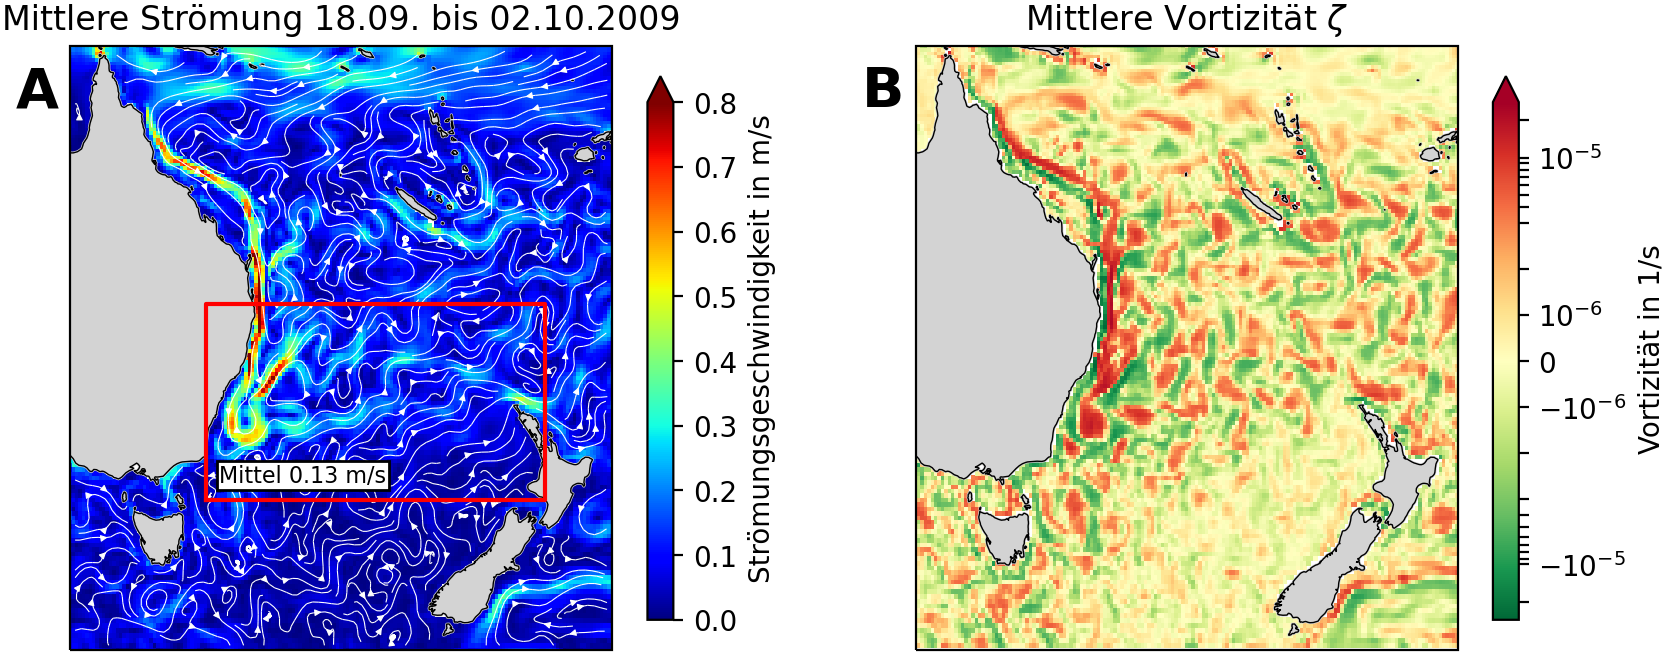
\includegraphics[width=\textwidth]{bilder/currents_mean.png}
\caption{A) Mittlere Strömung für den Untersuchungszeitraum im tasmanischen Meer mit höheren Geschwindigkeiten innerhalb der Tasmanischen Front (rote Box). Der Teil des Südpazifik-Wirbels trifft aus Nordöstlicher Richtung auf die Küste Queenslands, wird dann südlich abgelenkt und löst sich schließlich wieder Richtung Osten ab und bildet die tasmanische Front. B) Vortizität in derselben Region. Bereiche mit negativer Vortizität (grün) kennzeichnen zyklonale Wirbel, in denen der Nährstofftransport aus tieferen Schichten gefördert wird. } \label{fig:tasman_current}
\end{figure}
Abbildung \ref{fig:iron_transport}A zeigt die Eisenkonzentrationen im Ozean während und einige Tage nach Ende des Simulationszeitraums, die mit den stark vereinfachten Annahmen zu Transport und Durchmischung (sh. Kapitel \ref{sec:methods_advection}) berechnet wurden. Wie in Abb. \ref{fig:iron_transport} B zu erkennen ist, ändert sich die Verteilung der Konzentrationen durch Advektion nur in geringem Ausmaß. Die berechneten Konzentrationen weichen demnach geringfügig  von der Verteilung ab, die man erhält, wenn einfach die Staubdepositionen je Gitterpunkt zeitlich integriert werden. Dies bestätigt die Überschlagsrechnung von zuvor, dass der Strömungstransport nur über vergleichsweise kurze Distanzen passiert. Allerdings zeigt sich auch, dass die so berechneten Konzentrationen im Osten des Tasmanischen Meeres tatsächlich erhöht wurden. Darüber hinaus werden die Konzentrationen kontinuierlich in einem dem Grunde nach gleichen Muster transportiert. Nachdem am 27.09. beide Staub-Hauptereignisse größtenteils in direkter Nähe der ostaustralischen Küste Eisen eingetragen haben, werden zu den jeweils nächsten dargestellten Zeitpunkten die Konzentrationen in den Regionen östlich des 165'ten Breitengrads auf Höhe der Tasmanischen Front um bis zu 0.002 nM erhöht, weiter südlich leicht reduziert. \\

Angesichts des nur geringen Beitrags scheint es weiterhin unwahrscheinlich, dass die sehr hohen Chlorophyll-Konzentrationen am 1. und 2. Oktober maßgeblich durch den Staubeintrag vom 23. September eingeleitet wurden. Tatsächlich suggerieren Satellitenaufnahmen des 1. und 2. Oktobers (Abb. \ref{fig:satellite_october}, dass genau zu dieser Zeit in der Region möglicherweise weiterer Staub eingetragen wurde. Dieses potentielle Ereignis wurde allerdings nicht dokumentiert. Der zugehörige DustWatch Report \citep{Leys.2009b} resümiert, \textit{dass man in der Woche vom 28.09. bis 5. Oktober eine kurze Pause von Staubereignissen} hatte. Die Messstationen wiesen keine erhöhten Werte auf. Nichtsdestotrotz scheint der Zusammenhang vielversprechend (auch angesichts der u.U. sehr schnellen Reaktion des Phytoplanktons von 0-2 Tagen nach Staubeintrag, sh. Kapitel \ref{sec:auswertung_räuml_Muster} bzw. Abbildung \ref{fig:snapshot_fedep_chla}).
\begin{figure}
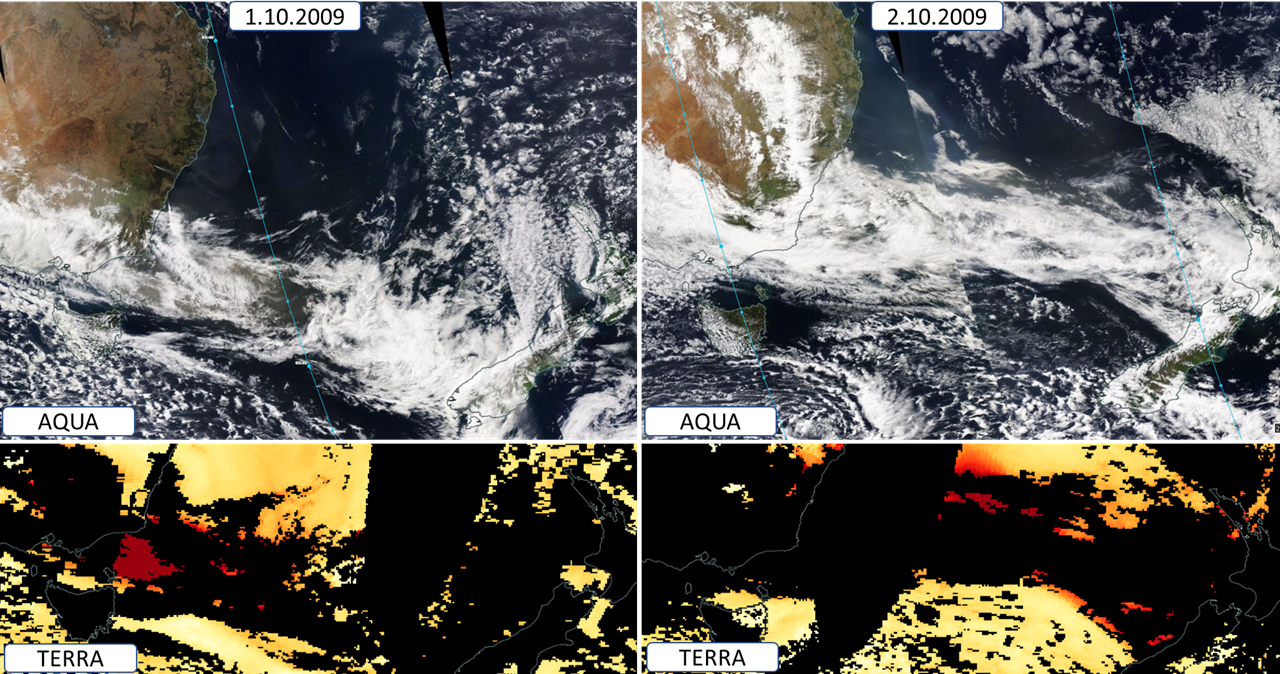
\includegraphics[width=\textwidth]{bilder/satellite_october.png}
\caption{Satellitenaufnahmen (AQUA/TERRA-MODIS) des Tasmanischen Meeres vom 1. und 2. Oktober. Oben: Echtfarbenbilder mit deutlicher dunkler Signatur im Wolkenband, insbesondere im westlichen Teil. Unten: Deutlich erhöhte Aeorosol optische Tiefe, am 2. Oktober entlang des gesamten Wolkenbandes. Alle Bilder wurden mithilfe des Tools NASA Worldview aufgenommen.} \label{fig:satellite_october}
\end{figure}
Auslöser dieser möglichen Staubemissionen sind gemäß Abbildung \ref{fig:october_weather} wieder starke nördliche/nordwestliche Winde, die mit zwei stark ausgeprägten, direkt aufeinander folgenden Kaltfronten im Zusammenhang stehen. Im westlichen Teil der Staatengrenze Northern Territory / Südaustralien sind die Windgeschwindigkeiten maximal. Etwas weiter östlich von dieser Region sind am 30. September auf der Satellitenaufnahme Terra MODIS (ca. 2 Uhr UTC) in Südaustralien auch Staubbewegungen zu erkennen. Mit dem Durchzug der Fronten gehen erhöhte Niederschläge einher, die die Löslichkeit des Eisens weiter erhöhen könnten. 
\begin{figure}
	\begin{minipage}[c]{0.3\textwidth}
		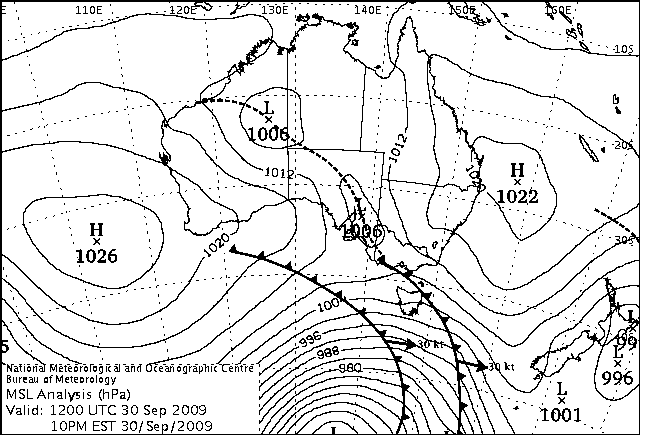
\includegraphics[width=\textwidth]{bilder/20090930T12_msl.png}
	\end{minipage}\hfill
	\begin{minipage}[c]{0.35\textwidth}
		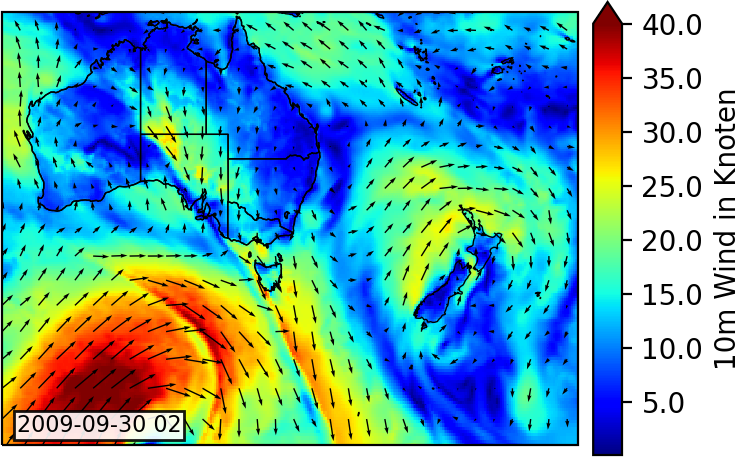
\includegraphics[width=\textwidth]{bilder/wind_october_small.png}
	\end{minipage}\hfill
	\begin{minipage}[c]{0.33\textwidth}
		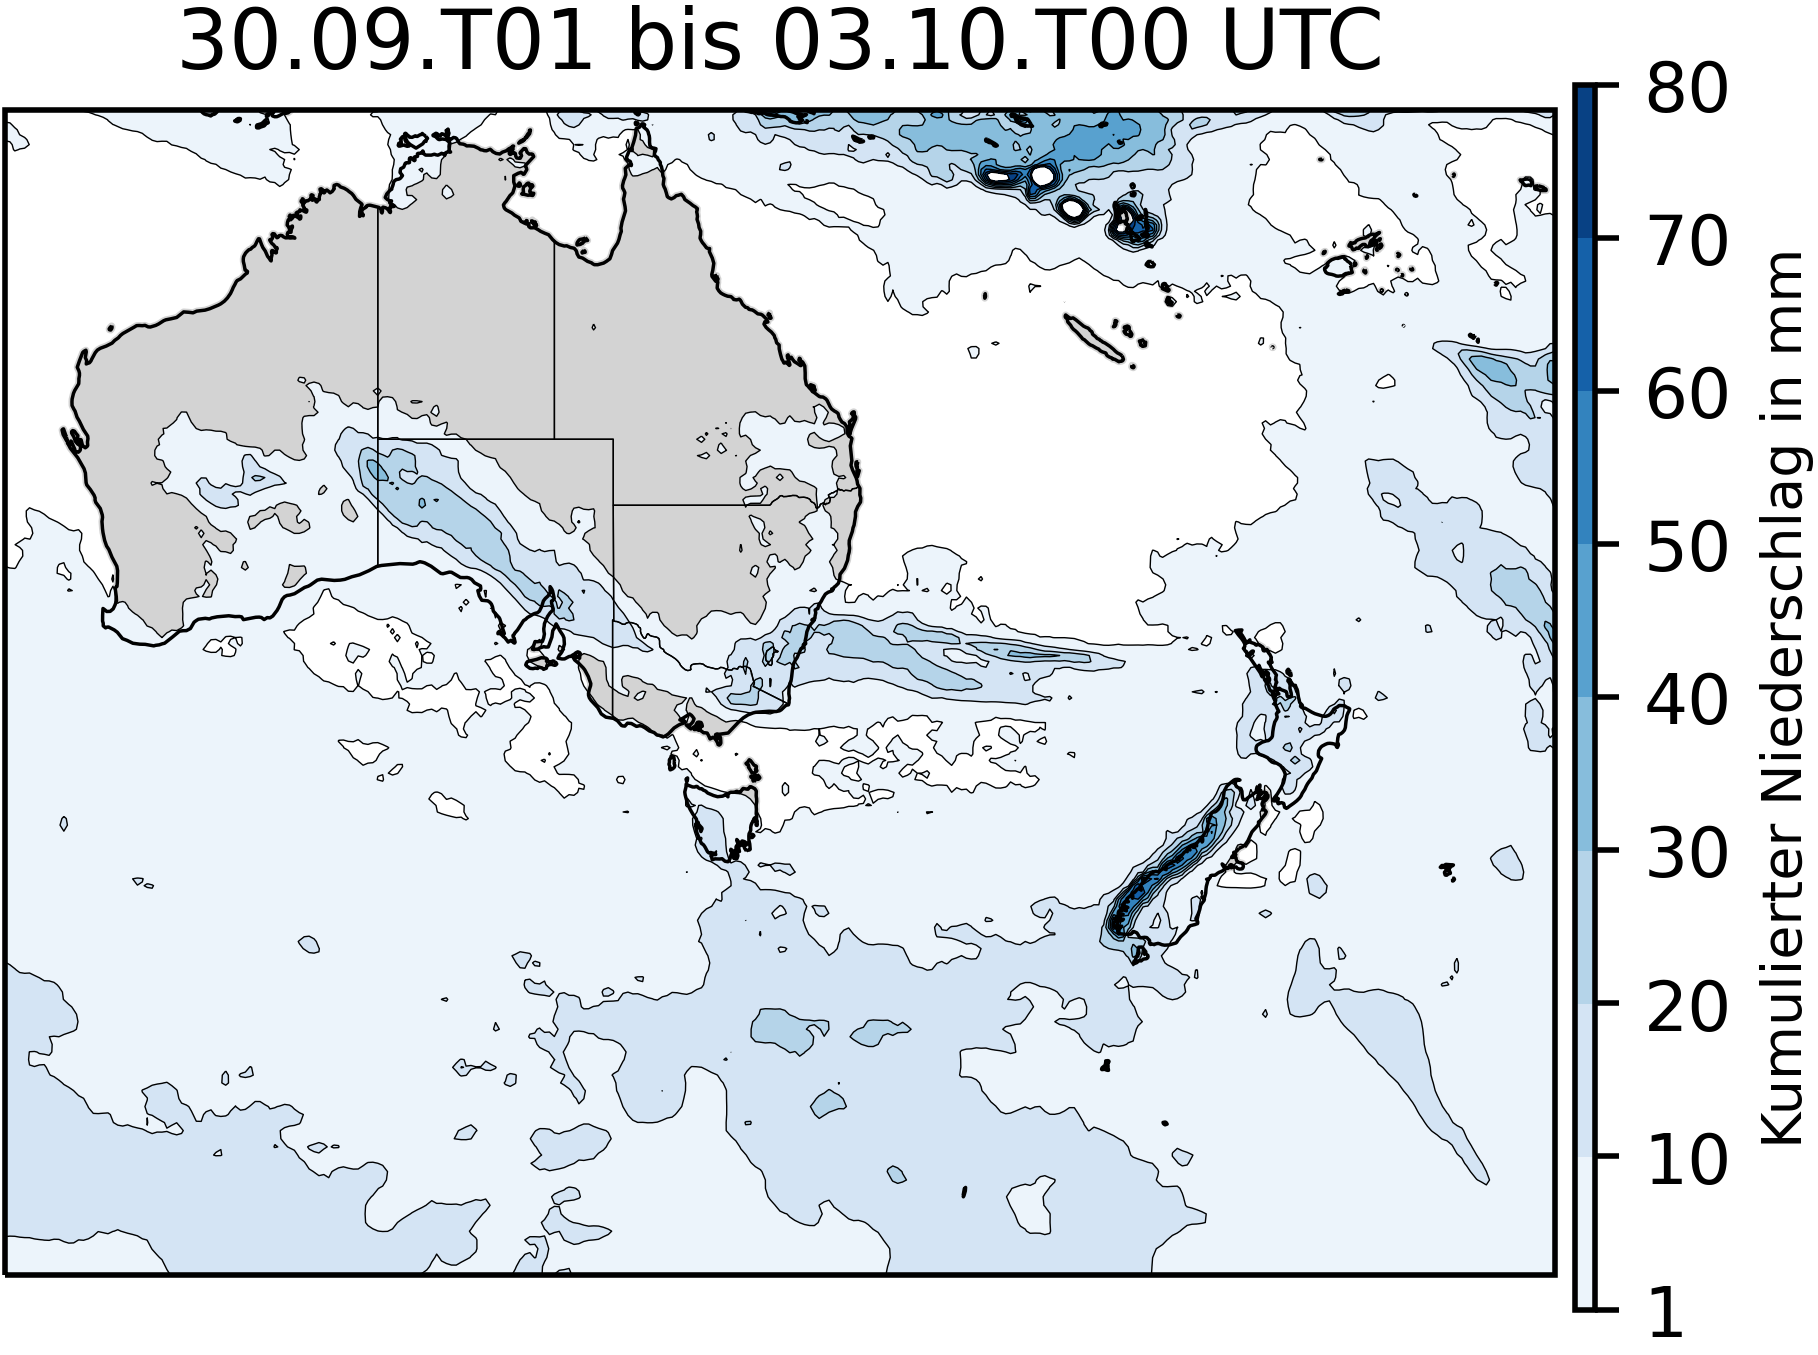
\includegraphics[width=\textwidth]{bilder/rain_october_small.png}
	\end{minipage}\hfill
	\caption{Eine Kurzübersicht zu den Wetterverhältnissen zum möglichen weiteren Staubereignis am 1. und 2. Oktober. Links: Bodendruckanalyse des BoM für 12 Uhr UTC des 30.09. mit der sehr deutlich ausgeprägten doppelten Kaltfront und zwei schwächeren Tiefdruckzonen in West- und Südaustralien. Mitte: Die auf dem Festland maximalen Windgeschwindkeiten laut Reanalysedaten (DOI: 10.24381/cds.adbb2d47) am 30.09. um 2 Uhr UTC. Rechts: Kumulierter Niederschlag für drei Tage ab dem 30.09.2009} \label{fig:october_weather}
\end{figure}
\subsection{Korrelationsanalyse} \label{sec:correlation_analysis}
Auf Basis der mithilfe der Advektionsgleichung abgeschätzten täglichen Eisenkonzentrationen bzw. deren Veränderungen wird nun die bereits angekündigte Korrelationsanalyse durchgeführt.
\begin{figure}
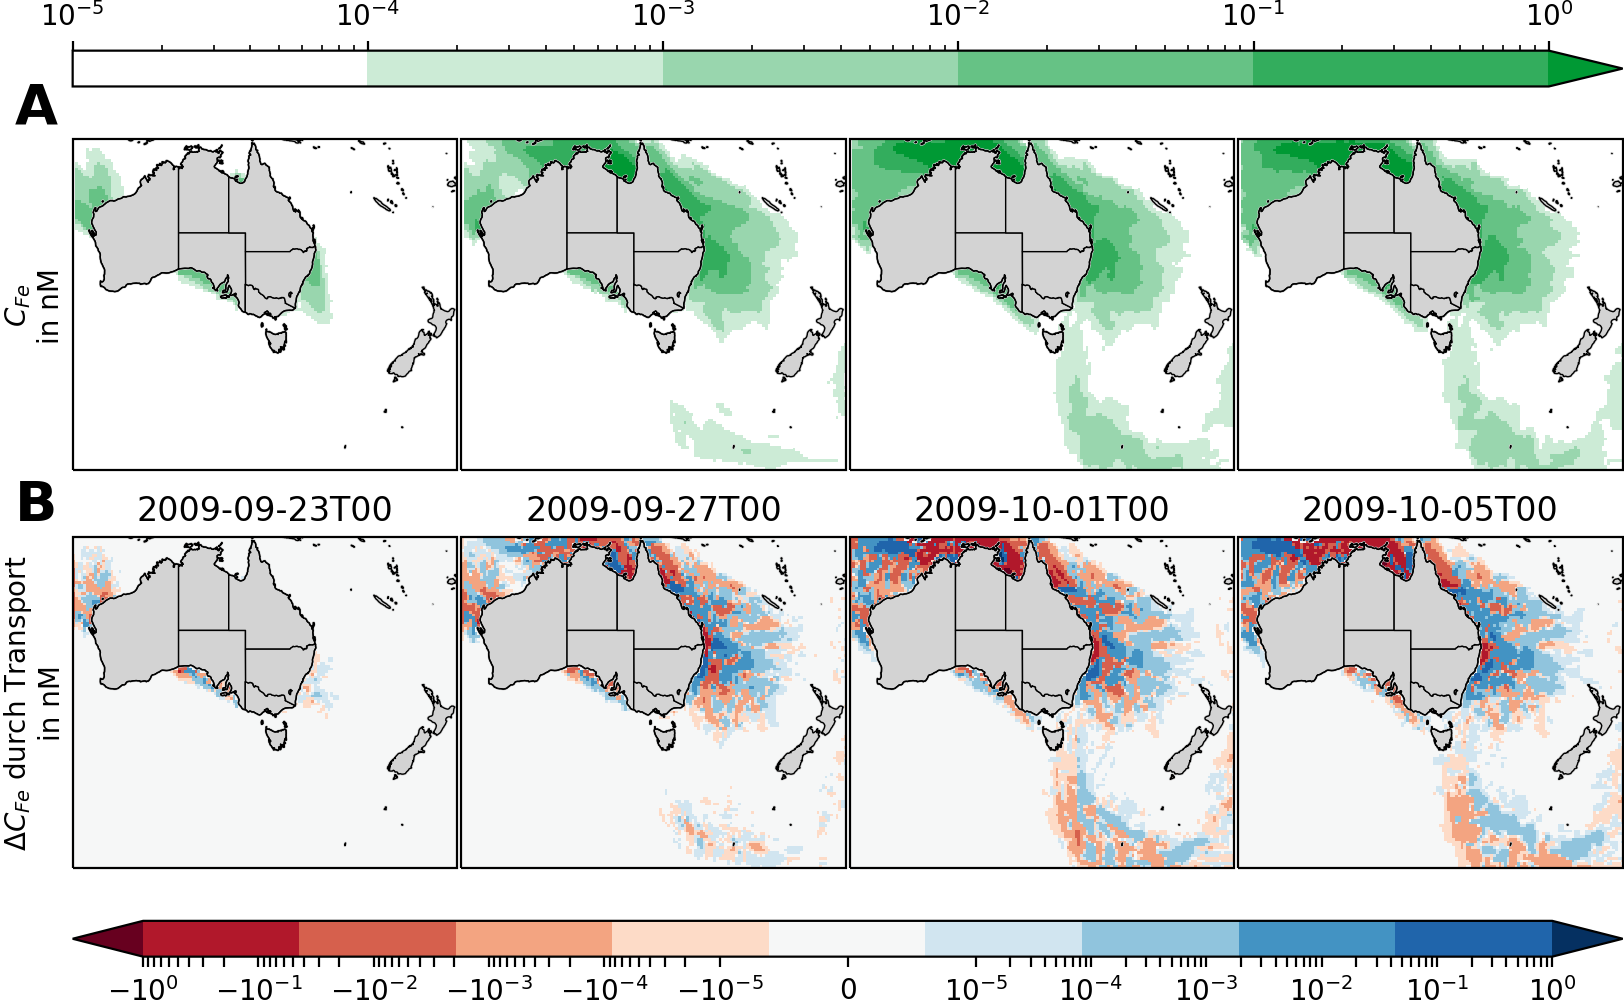
\includegraphics[width=\textwidth]{bilder/iron_transport.png}
\caption{} \label{fig:iron_transport}
\end{figure}
\section{Zusammenfassung und Ausblick}
\newpage
\printbibliography
\appendix
\section{Anhang}

%\addcontentsline{toc}{section}{Abbildungsverzeichnis}
%\listoffigures
%\addcontentsline{toc}{section}{Tabellenverzeichnis}
%\listoftables
\section{Danksagung}
\nocite{*}
\end{document}
